%============================================================================
% tento soubor pouzijte jako zaklad
% (c) 2008 Michal Bidlo
% E-mail: bidlom AT fit vutbr cz
%============================================================================
% kodovaní: utf-8 (zmena prikazem iconv, recode nebo cstocs)
%----------------------------------------------------------------------------
% zpracování: make, make pdf, make desky, make clean
% připomínky posílejte na e-mail: bidlom AT fit.vutbr.cz
% vim: set syntax=tex encoding=utf-8:
%============================================================================
\documentclass[english,cover]{fitthesis} % odevzdani do wisu - odkazy, na ktere se da klikat
%\documentclass[cover,print]{fitthesis} % pro tisk - na odkazy se neda klikat
%\documentclass[english,print]{fitthesis} % pro tisk - na odkazy se neda klikat
%      \documentclass[english]{fitthesis}
% * Je-li prace psana v anglickem jazyce, je zapotrebi u tridy pouzit 
%   parametr english nasledovne:
%      \documentclass[english]{fitthesis}
% * Neprejete-li si vysazet na prvni strane dokumentu desky, zruste 
%   parametr cover

% zde zvolime kodovani, ve kterem je napsan text prace
% "latin2" pro iso8859-2 nebo "cp1250" pro windows-1250, "utf8" pro "utf-8"
%\usepackage{ucs}
\usepackage[utf8]{inputenc}
\usepackage[T1, IL2]{fontenc}
\usepackage{url}
\DeclareUrlCommand\url{\def\UrlLeft{<}\def\UrlRight{>} \urlstyle{tt}}

%zde muzeme vlozit vlastni balicky
\usepackage{amsmath}
\usepackage{amsthm}
\usepackage{color}
\usepackage{comment}
\usepackage{graphicx}
\usepackage{caption}
\usepackage{subcaption}
\usepackage{multirow}
\usepackage{changepage}
\newtheorem{math_def}{Definition}[chapter] % 3. parametr zajisti cislovani "<sekce>.<číslo definice>"
\newcommand{\term}[1]{\emph{#1}}           % novy termin v textu prace
\newcommand{\srccode}[1]{{\tt #1}}         % fragment zdrojaku v textu
\newcommand{\vars}[1]{{\bold{#1}}}         % matematicke vyrazy - mnozina promennych
\newcommand{\bnfconst}[1]{``\textbf{#1}''} % BNF literal / konstanta
\newcommand{\bnfgroup}[1]{\textit{#1}}     % BNF skupina
\newcommand{\ignore}[1]{}                  % komentar v radku
\newcommand{\todo}[1]{{\color{red}#1}}
\newcommand{\uncertain}[1]{{\color{magenta}#1}}
\newcommand{\note}[1]{{\color{green}#1}}

% prostredi pro vlozeni prilohy na strance velikosti A3
\usepackage{afterpage}
\newenvironment{hugepage}
  {\clearpage
   %\pagestyle{empty}  % turn off display of page numbers, headers, ...
   %\changepage{247mm}{370mm}{25mm}{25mm}{}{}{}{}{}} % switch to A3
   \changepage{}{210mm}{}{}{}{}{}{}{}}
  {%\addtocounter{page}{-1} % decrement "page" counter variable by 1
   \clearpage
   %\changepage{160mm}{247mm}{25mm}{25mm}{}{}{}{}{}} % back to A4
   \changepage{}{-210mm}{}{}{}{}{}{}{}}

% SP komentar co se hodi zohlednit ve finalni diplomce


% =======================================================================
% balíček "hyperref" vytváří klikací odkazy v pdf, pokud tedy použijeme pdflatex
% problém je, že balíček hyperref musí být uveden jako poslední, takže nemůže
% být v šabloně
\ifWis
\ifx\pdfoutput\undefined % nejedeme pod pdflatexem
\else
  \usepackage{color}
  \usepackage[unicode,colorlinks,hyperindex,plainpages=false,pdftex]{hyperref}
  \definecolor{links}{rgb}{0.4,0.5,0}
  \definecolor{anchors}{rgb}{1,0,0}
  \def\AnchorColor{anchors}
  \def\LinkColor{links}
  \def\pdfBorderAttrs{/Border [0 0 0] }  % bez okrajů kolem odkazů
  \pdfcompresslevel=9
\fi
\fi

% Informace o praci/projektu
%---------------------------------------------------------------------------
\projectinfo{
  % Prace
  project=DP,            % typ prace BP/SP/DP/DR
  year=2013,             % rok
  date=\today,           % datum odevzdani
  % Nazev prace
  title.cs={Aplikace Bayesovských sítí},     % nazev prace v cestine
  title.en={Bayesian Networks Applications}, % nazev prace v anglictine
  % Autor
  author={David Chaloupka},   % jmeno prijmeni autora
  author.title.p=Bc.,         % titul pred jmenem (nepovinne)
  %author.title.a=PhD,        % titul za jmenem (nepovinne)
  % Ustav
  department=UITS, % doplnte prislusnou zkratku: UPSY/UIFS/UITS/UPGM
  % Skolitel
  supervisor=František V. Zbořil, % jmeno prijmeni skolitele
  supervisor.title.p=doc.~Ing.,   % titul pred jmenem (nepovinne)
  supervisor.title.a={CSc.},      % titul za jmenem (nepovinne)
  %Klicova slova, abstrakty, prohlaseni a podekovani je mozne definovat 
  %bud pomoci nasledujicich parametru nebo pomoci vyhrazenych maker (viz dale)
  %===========================================================================
  %Klicova slova
  keywords.cs={Bayesovská síť, pravděpodobnost, inference, učení struktury, strojové učení, spam.}, %klicova slova v ceskem jazyce
  keywords.en={Bayesian network, probability, inference, structure learning, machine learning, spam.}, %klicova slova v anglickem jazyce
  %Abstract
  abstract.cs={Tato diplomová práce se zabývá možnými aplikacemi Bayesovských sítí. Nejprve se zaměřuje na obecnou teorii pravděpodobnosti, později na úrovni matematiky vysvětluje samotnou teorii Bayesovských sítí, přístupy k inferenci a k učení včetně pochopení silných a~slabých stránek daných technik. V praktické části je kladen důraz na aplikace vyžadující učení Bayesovské sítě, jednak ve smyslu učení parametrů a jednak ve smyslu struktury.}, % abstrakt v ceskem jazyce
  abstract.en={This master's thesis deals with possible applications of Bayesian networks. The theoretical part is mainly of mathematical nature. At first, we focus on general probability theory and later we move on to the theory of Bayesian networks and discuss approaches to inference and to model learning while providing an explanation of pros and cons of these techniques. The practical part focuses on applications suitable for learning a Bayesian network, both in terms of network parameters as well as structure.}, % abstrakt v anglickem jazyce
  %Prohlaseni
  declaration={Prohlašuji, že jsem tuto diplomovou práci vypracoval samostatně pod vedením pana doc.~Ing. Františka V. Zbořila, CSc.},
  %Podekovani (nepovinne)
  acknowledgment={Na tomto místě bych rád poděkoval svému vedoucímu, docentu Františku V. Zbořilovi, za cenné rady, odborné vedení a vstřícný přístup v nesnázích při řešení této práce.} % nepovinne
}


\begin{document}
  % Vysazeni titulnich stran
  % ----------------------------------------------
  \maketitle
  % Obsah
  % ----------------------------------------------
  \tableofcontents
  
  % Seznam obrazku a tabulek (pokud prace obsahuje velke mnozstvi obrazku, tak se to hodi)
  % \listoffigures
  % \listoftables 

  % Text prace
  % ----------------------------------------------

  








%end-of-inserted-header
%=========================================================================
% (c) Michal Bidlo, Bohuslav Křena, 2008

\chapter{Introduction}
\vspace{-0.7mm}
Bayesian networks are a subclass of probabilistic graphical models and serve as a~tool for modeling joint probability distributions of random variables. Bayesian networks were originally used to evaluate medical data of a patient in order to determine the probability of him having a certain disease which is a situation with many unknowns, eg. missing medical history or unknown results of medical tests that haven't been done. Since then there have been many other applications such as inspection of pedigree trees in genetics or discovery of protein signaling mechanisms based purely on statistical data.

The main advantages of Bayesian networks lie in the fact that they are easy to interpret, even for a non-specialist, and in their inherent property that they can represent joint probability distributions in a very compact way in terms of space complexity. Construction of a Bayesian network for some concrete domain is a complicated task demanding complex algorithms, enough input data and, in many cases, expert knowledge. Another problem is providing answers to queries regarding the probability distribution induced by a given Bayesian network, so called inference.

The aim of this thesis is to present techniques of learning Bayesian networks, both in terms of conditional probability tables, ie. model parameters, as well as in terms of structure, and to demonstrate their possible applications. Inference techniques are narrowed down to stochastic approaches because other ways are complex even in the most basic form. Still, all approaches to inference will be mentioned at least on the level of basic concept, since it is a fundamental part of the theory of Bayesian networks.

\medskip

Chapter 2 serves as an introduction to the fundamentals of the probability theory and provides necessary foundations for understanding the rest of this thesis, including the used mathematical notation.

Chapter 3 discusses the theory of Bayesian networks. First, the motivation for using Bayesian networks is explained, followed by an overview of the inference methods and by survey of model learning techniques in terms of parameters as well as structure.

In chapter 4 I will introduce the realization output of this thesis with focus on the overall design and philosophy. This chapter should be partly seen as program documentation.

Chapter 5 discusses selected applications of parameter and structure learning of Bayesian networks. The first application is a study of optimal parameter settings of the model learning procedures for networks and datasets of various sizes. The second application uses model learning as a tool to discover the main causes of criminality. The third application explores the option of using a generalized Naïve Bayes model for spam filtering.

Appendix A provides an overview of the mathematical notation used in this thesis.

Appendix B describes content of the CD enclosed with this thesis.































\chapter{Preliminaries}
This chapter will present theoretical foundations for understanding Bayesian networks and for performing computation over them. Studying Bayesian networks (further abbreviated as BNs) is challenging both because of necessary mathematical rigor as well as for the need of efficient non-trivial algorithms to construct them and to provide answers for probability queries. In case of some formulas their mathematical derivation will be presented because, I believe, it provides useful insight into the underlaying theory. In other cases we will jump straight to the practical conclusion needed in order to algorithmically solve the problem at hand because the derivation is either very difficult or the process itself is uninteresting for a~non-mathematician and would unnecessarily prolong the thesis or even obfuscate the topic.

First will be established notation used in this thesis and necessary overview of probability theory. Then we will move on to the theory of Bayesian networks, explain their advantages and proceed to inference and model learning techniques.



\section{Philosophical views}
Probability of an event is usually interpreted as the degree of belief in occurrence of that particular event, eg. probability of a fair die rolling a six is $1/6$. Although probability is expressed as a~real number between zero and one, the ground truth is that in the end one and only one \emph{concrete} event is observed. In the case of a die, one concrete number is rolled regardless what the probabilities were. Although our intuition and general experience proves it to be true in our macroscopic world, objects in the microscopic world of quantum mechanics actually are probabilistic in nature and, a particle for example, is in many quantum states at the same time. The particle is then described by a complex \term{wave function} $\Psi(x,y,z,t)$ and $\vert\Psi(x,y,z,t)\vert^2$ describes \term{density probability} of the particle as a function of space-time coordinates~\cite[p.~1044]{hrw_physics}. Despite the obvious differences, certain qualities of both these worlds can be described by the same mathematical apparatus which is probability theory.

Somewhat close to probability theory is the theory of fuzzy sets which operates with membership functions. These functions describe degrees of truth, eg. that a person is regarded as young or old. The main difference, when compared to probability, is that in fuzzy sets theory an object may have more than one quality to some degree and there is no ground truth or observation that would strictly place a person into one single category.


\section{Probability distributions}
Let's begin by defining what a probability distribution is when there is only one single random variable.
\begin{math_def}\label{def_prob_distribution}
    $P(X)$ is discrete probability distribution of discrete random variable $X$ such that:
    \begin{itemize}
        \item $X$ can be assigned any value from the set $val(X) = \lbrace x_1, x_2, \dots \rbrace$ which is finite or denumerable.
        \item $\forall x_i \in val(X): P(X = x_i) \geq 0$
        \item $\Bigl( \sum_i P(X = x_i) \Bigr) = 1$
    \end{itemize}
\end{math_def}

Notice that random variables are denoted by capital letters $X, Y, E$ etc., concrete values of random variables (assignments or instantiations) are denoted by small letters such as $x$. Further we will use bold capital letters to denote sets of random variables such as $\vars{X}$ and their instantiation with bold small letters such as $\vars{x}$.

Probability distributions of more than one random variable are called \term{joint probability distributions}. For example if we were to study a simultaneous throw with two dices, black and white, we would get joint probability distribution $P(X_{black},X_{white})$. In this probability distribution we know how likely every single outcome of a throw is. In this case there are $6 \times 6 = 36$ possibilities so the probability distribution $P(X_{black},X_{white})$ would have 36 entries if represented by a table.

So far we have described so called \term{prior probabilities} which are applicable in situations when no observation has been made and hence everything is governed purely by probability. If, on the other hand, we observe that some random variable takes on a concrete value (eg. the weather today is sunny) then we speak about \term{posterior probability} or \term{conditional probability} distribution.
Posterior and prior probability distributions are not the same in general because observation of a~variable may affect distribution of other variables as we will see later in context of flow of probabilistic influence in Bayesian networks.
Conditional probability distribution of variables $\vars{X}$ depending on variables $\vars{E}$ is denoted $P(\vars{X}\mid\vars{E})$ and such expression is usually read as \uv{probability of $\vars{X}$ given $\vars{E}$} where $\vars{E}$ are called \term{evidence} or \term{observed} variables. Conditional probability distribution can be seen as a collection of probability distributions over variables $\vars{X}$ for every possible instantiation $\vars{e}$ of variables $\vars{E}$.


\section{Factors}
When reasoning about Bayesian networks we express probability distributions as so called \term{factors}. Factors are interesting for us because factor operations, among other uses, correspond to mathematical operations we need to perform with probability distributions in order to answer queries in a~Bayesian network.
\begin{math_def}\label{def_factor}
    Factor $\phi$ is a function $\phi: X_1 \times X_2 \times \dotsm \times X_k \rightarrow \mathbb{R}_0^+$. The non-empty set $\lbrace X_1, X_2, \dots, X_k \rbrace$ is called scope of the factor $\phi$.
\end{math_def}
According to the definition of a factor and to the definition \ref{def_prob_distribution} of a discrete probability distribution, probability distributions are special cases of factors. They both require their values to be non-negative and, in addition, every probability distribution must sum to one. A~factor, of course, may sum to one too in which case we say it is \term{normalized}.

Factor representation of a joint probability distribution $P(X,\dots,Z)$ is straightforward\,--\,simply put $\phi(x,\dots,z) = P(x,\dots,z)$ for every assignment $x,\dots,z$ of variables $X,\dots,Z$. In this case probabilities of all possible assignments must necessarily sum to one since $P(X,\dots,Z)$ is a~probability distribution. For further reference, this summation is denoted $\sum_{X,\dots,Z} P(x,\dots,z) = 1$.

Let's examine the case of a conditional probability distribution $P(\vars{X}\mid\vars{E})$. Suppose that, according to the established notation, $\vars{X}$ and $\vars{E}$ are sets of variables rather than single variables. Then $scope(\phi) = \vars{X} \cup \vars{E}$ but probabilities of all possible assignments to $\vars{X}$ and $\vars{E}$ doesn't sum to one! This is because the conditional probability distribution $P(\vars{X}\mid\vars{E})$ is more like a collection of probability distributions of variables $\vars{X}$ for every assignment to $\vars{E}$. So, for any concrete assignment $\vars{e}$ of evidence variables $\vars{E}$, the probability distribution $P(\vars{X}\mid\vars{e})$ again sums to one, ie. $\sum_\vars{X} P(\vars{x}\mid\vars{e}) = 1$.

\medskip
There are 4 operations over factors we will need further in this thesis\,--\,pointwise product, marginalization, conditioning and renormalization. Formal definitions below are derived from description of these operations in~\cite{russell_norvig_ed2, pgm}

\subsubsection{Pointwise product}
Pointwise product of factors $\phi_1$ and $\phi_2$ is a factor $\psi$, denoted $\psi = \phi_1 \cdot \phi_2$, defined as follows. The scope of $\psi$ is $scope(\phi_1) \cup scope(\phi_2)$. Let $scope(\phi_1) = \lbrace X_1, \dots, X_m, Y_1, \dots, Y_n \rbrace$ and $scope(\phi_2) = \lbrace Y_1, \dots, Y_n, Z_1, \dots, Z_k \rbrace$ where $\lbrace X_1, \dots, X_m \rbrace$ and $\lbrace Z_1, \dots, Z_k \rbrace$ are disjoint. For every assignment $x_1, \dots, x_m, y_1, \dots, y_n, z_1, \dots, z_k$ of variables in $scope(\psi)$ the value of $\psi(\cdot)$ is given as:
$$\psi(x_1, \dots, x_m, y_1, \dots, y_n, z_1, \dots, z_k)
= \phi_1(x_1, \dots, x_m, y_1, \dots, y_n) \cdot \phi_2(y_1, \dots, y_n, z_1, \dots, z_k)
$$

Please note that it is also possible for the sets $\lbrace X_i \rbrace_i, \lbrace Y_i \rbrace_i,\lbrace Z_i \rbrace_i$ to be empty (of course, according to the definition~\ref{def_factor}, any factor must have at least one variable in its scope).

\subsubsection{Marginalization}
Marginalization of a factor $\phi$ over variables $\vars{Y}$ is operation of summing out these variables, effectively producing factor $\psi$. Then $scope(\psi) = scope(\phi) \setminus \vars{Y}$ and for every assignment $\vars{x}$ of variables in $scope(\phi)$ holds that $\psi(\vars{x}) = \sum_\vars{Y} \phi(\vars{x},\vars{y})$.

\subsubsection{Conditioning}
Conditioning is operation used when there is some observed evidence $\vars{e}$ of variables $\vars{E}$. By conditioning we set probabilities of all events inconsistent with observed evidence to 0. Of~course, the resulting factor will not be normalized in general.

\subsubsection{Renormalization}
Renormalization of a factor $\phi$ ensures that all values of the factor sum to one. Suppose that $\vars{X} = scope(\phi)$ and let $\alpha = \sum_\vars{X} \phi(\vars{x})$ be normalizing constant. Values of the resulting factor $\psi$ are given for every assignment $\vars{x}$ of variables $\vars{X}$ as $\psi(\vars{x}) = \phi(\vars{x}) / \alpha$.

It may be useful to point out that renormalization makes sense only for factors that don't represent conditional probability distributions.



































\chapter{Theory of Bayesian networks}
In this chapter we will first discuss the reasons for using Bayesian networks. Then we will move on to various inference methods and to methods of model learning, both in terms of model parameters as well as in terms of structure.

Let's ask the question why to use Bayesian networks? What do they bring us? First of all, having a complicated joint probability distribution with many random variables inevitably leads to an enormously large table that would represent such probability distribution. Let's assume we have binary random variables $X_1, \dots, X_k$. Then to represent the joint probability distribution $P(X_1, \dots, X_k)$ we would need a table with $2^k$ entries. This exponential growth brings several problems:
\begin{itemize}
    \item Table completely describing a joint probability distribution may be too big to store. That is because the table would hold probability of every possible event separately in its own record.
    \item Even if the table could be stored, performing calculations over it (e.g. factor marginalization or factor multiplication) would not be efficient. In fact, operations such as exact inference are known to be NP-hard in the number of variables~\cite{pgm}.
    \item In order to construct probability table for a joint probability distribution:
    \begin{enumerate}
        \item[a)] We would require a huge amount of training data to create an accurate statistical model from, since we would essentially count occurrences of every single event (ie. of \emph{each possible} instantiation of all random variables) and finally divide these counts by the total number of all training examples.
        \item[b)] We would need a human expert to determine the probability of every possible assignment of random variables. This is generally not possible because all probabilities would be near to zero and human experts are simply not able to correctly capture probabilities on this level~\cite{pgm}.
    \end{enumerate}
\end{itemize}

As will be shown later, Bayesian networks couple with the problem of exponential growth of record counts in probability tables by having several smaller local conditional probability distributions (factors) based on dependencies between random variables. Product of all these conditional probabilities (factors) in the entire network gives the underlaying joint probability distribution which would, if represented naively, require an exponentially large table.



\begin{math_def}\label{def_bayesian_network}
    Bayesian network is a tuple $(\mathcal{G}, \Theta)$. $\mathcal{G}$ is a directed acyclic graph where each node represents a~random variable and oriented edges between nodes express direct dependencies between random variables represented by the connected nodes. $\Theta$ are parameters of the network representing for each node $X$ its probability distribution conditioned on its immediate parents, denoted $P(X \mid Parents(X))$.
\end{math_def}

The definition of Bayesian network (further abbreviated BN) implies several things. Acyclic and directed properties tell us that there is a hierarchy of nodes in terms of parent-child or predecessor-successor relation, meaning that a random variable $C$ is dependent on its parent random variables $\lbrace P_1, \dots, P_m \rbrace$ (denoted $Parents(C)$). This conditional probability distribution $P(C \mid Parents(C))$ is usually\footnote{For purposes of this thesis, we assume probability distributions of discrete, not continuous, variables whose events are from a finite set. Such probability distribution can be expressed by a table.} expressed via a \term{Conditional Probability Table (CPT)} that defines probability distribution of variable $C$ for every possible assignment of variables $Parents(C)$. Of course, for every assignment $p_1,\dots,p_m$ of variables $Parents(C)$ must hold that $\sum_C P(c \mid p_1, \dots, p_m) = 1$. Otherwise $P(C \mid Parents(C))$ would not be a~probability distribution (by definition~\ref{def_prob_distribution}).

We say that Bayesian network $(\mathcal{G}, \Theta)$ with nodes $\lbrace X_1, \dots, X_k\rbrace$ induces joint probability distribution $P(X_1, \dots, X_k)$ as follows:
\begin{equation}\label{eq:bn_joint}
    P(X_1, \dots, X_k) = \prod_{i=1}^k P(X_i \mid Parents(X_i))
\end{equation}
Equivalent statement is that $P(X_1, \dots, X_k)$ factorizes over a BN $(\mathcal{G}, \Theta)$ if the equation \eqref{eq:bn_joint} holds. This is because the terms $P(X_i \mid Parents(X_i))$ are \term{factors} and by constructing a~Bayesian network we can factorize otherwise very space-consuming CPD of $P(X_1, \dots, X_k)$ into several smaller CPDs $P(X_i \mid Parents(X_i))$, one for every node $X_i$.

I have devised a proof that $P(X_1, \dots, X_k)$ induced by a BN is indeed a probability distribution, when assuming that every factor $P(X_i \mid Parents(X_i))$ is also a probability distribution. Main purpose of this proof is to provide the reader with some familiarity when mathematically reasoning about BNs because similar tricks will be used later on. Core of the proof is to show that both axioms of a probability distribution (Definition \ref{def_prob_distribution}) are satisfied\footnote{Because of long expressions in the following two paragraphs, $Pars(X)$ denotes $Parents(X)$.}:
\begin{enumerate}
   \item $P(X_1, \dots, X_k) \geq 0$:
       Trivial since factors $P(X_i \mid Parents(X_i))$ are assumed to be valid probability distributions. Then, by definition of probability distribution~\ref{def_prob_distribution}, we know that $\forall i: P(X_i \mid Parents(X_i)) \geq 0$. And product of non-negative numbers (factors) is also non-negative, ie. $\prod_{i=1}^k P(X_i \mid Parents(X_i)) \geq 0$.
   \item $\sum P(x_1, \dots, x_k) = 1$: If the remaining variables $X_1, \dots, X_k$ are all independent, then by definition of independent random variables $P(X_1, \dots, X_k) = P(X_1) \dotsm P(X_k)$. So the sum can be written as $\sum P(x_1, \dots, x_k) = \sum_{X_1} P(x_1) \sum_{X_2} P(x_2) \dotsm \sum_{X_k} P(x_k)$. By assumption, all factors are valid probability distributions, so $\sum_{X_k} P(x_k) = 1$. Then $\sum_{X_1} P(x_1) \sum_{X_2} P(x_2) \dotsm \sum_{X_k} P(x_k) = \sum_{X_1} P(x_1) \sum_{X_2} P(x_2) \dotsm 1$. Thus we have eliminated variable $X_k$ and transformed the problem to $\sum P(x_1, \dots, x_{k-1}) = 1$. By eliminating all remaining variables the same way, we get $\sum P(x_1, \dots, x_k) = 1$.
       
       If there is a direct dependency between some two variables let's relabel the variables so that their indices correspond to a topological sort of the given BN (every BN is a~DAG, so a topological sort exists).  Then we can rewrite the inspected summation in the form $\sum P(x_1, \dots, x_k) = \sum_{X_1} P(x_1 | Pars(X_1)) \sum_{X_2} P(x_2 | Pars(X_2)) \dotsm \sum_{X_k} P(x_k | Pars(X_k))$ because, thanks to the topological sort, all parent variables of a variable $X_i$ must have smaller index that $i$. Also note that the maximal element $X_k$ has no child. By assumption, $P(X_k \mid Pars(X_k))$ is a probability distribution, so $\sum_{X_k} P(x_k \mid Pars(X_k)) = 1$. By substituting the term $\sum_{X_k} P(x_k \mid Pars(X_k))$ in the summation we eliminate the variable $X_k$ and transform the problem to question if $\sum P(x_1, \dots, x_{k-1}) = 1$ which we approach recursively.
\end{enumerate}


\section{Flow of probabilistic influence}
To describe how observing certain facts propagates through a Bayesian network and how it affects probability distributions of unobserved variables on qualitative level, we introduce \term{flow of probabilistic influence}. Flow of influence also enables us to formally capture conditional dependency and/or independency of random variables in a BN given some facts.
\begin{math_def}
    Let $(\mathcal{G}, \Theta)$ be a Bayesian network with nodes $X_1, X_2, \dots, X_k$ and let $\vars{Z}$ be a~set of observed variables, where $\vars{Z} \subseteq \lbrace X_1, \dots, X_k \rbrace$. A connected undirected trail $X_a - X_{a+1} - \dots - X_b$ given facts $\vars{Z}$ is active if and only if
    \begin{itemize}
        \item For every so called \uv{V-structure} $X_{i-1} \rightarrow X_i \leftarrow X_{i+1}$ on the trail is $X_i \in \vars{Z}$.
        \item No other node of given trail is in $\vars{Z}$.
    \end{itemize}
    Notes: V-structure is defined as a segment of trail in form $X_{i-1} \rightarrow X_i \leftarrow X_{i+1}$ (in this case, edge directions do matter). Also note that the trail may contain duplicate nodes.
\end{math_def}

\begin{math_def}
    Let $(\mathcal{G}, \Theta)$ be a Bayesian network, $X,Y$ two of its nodes and $\vars{Z}$ observed variables. We say that $X,Y$ given $\vars{Z}$ are d-separated in $\mathcal{G}$ iff there is no active trail between $X$ and $Y$ given $\vars{Z}$.
    
    Note: $X$ and $Y$ being d-separated given $\vars{Z}$ is equivalent to $X$ and $Y$ being conditionally independent given $\vars{Z}$, denoted $X \perp Y \mid \vars{Z}$.
\end{math_def}

By using d-separation (direction-dependent separation) we can quite elegantly determine if observation of a variable $X$ can or cannot affect distribution of some other random variable. Clearly, two random variables that are directly connected are dependent. But we can also examine other than these intuitively obvious relations. Also, please note that whether two random variables $X,Y$ are independent in Bayesian network depends on our observations $\vars{Z}$ as it can activate some trails in V-structures just as it can deactivate direct segments of other trails.

To understand better the notion of active trails and d-separation we will refer to examples in Figure~\ref{fig:bn_d-separation}. In Figure~\ref{fig:bn_d-separation_a} you can see a Naïve Bayes model in which all feature variables $X_i$ and $X_j$ are conditionally independent given class variable $C$ because knowing the class variable deactivates all trails between $X_i$ and $X_j$.
In Figure~\ref{fig:bn_d-separation_traffic} we can see an activated V-structure $R\rightarrow T \leftarrow A$, provided the variable $T$ is observed. Intuitively, when we know whether there is a traffic jam then an accident decreases probability of being it in a rush hour because an accident is sufficient to cause a traffic jam by itself, formally $R \not\perp A \mid T$. To go one step further, if it is not a rush hour then knowing there is a~traffic jam increases the probability of there being an accident which causally means higher probability of hearing sirens, hence $R\not\perp H \mid T$. The argumentation involving activated V-structures is an example of \term{inter-causal} reasoning (causes with common effect are conditionally dependent given the effect variable).
In Figure~\ref{fig:bn_d-separation_abstract} we will examine three more complicated cases of interest. The first selected case is $A \not\perp C \mid B, G$ because of the active trail $A-D-F-G-F-C$ (node $F$ is twice on the trail which is perfectly legal). The second selected case is $A \perp F \mid B, D$ because both possible trails between $A$ and $F$ are deactivated. The third selected case is $E \not\perp B \mid F, C$ because there is an active trail $E-F-D-A-B$.

\begin{center}
\begin{figure}[h]
    \begin{subfigure}[b]{0.42\linewidth}
        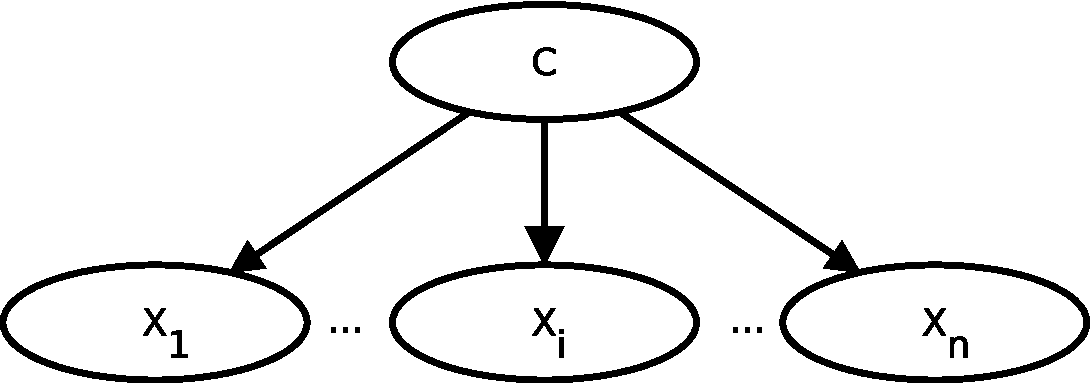
\includegraphics[scale=0.4]{fig/bn-naive-bayes}
        \caption{General Naïve Bayes model in which holds $X_i \perp X_j \mid C$ for $i \neq j$}
        \label{fig:bn_d-separation_a}
    \end{subfigure}
    \qquad\qquad\qquad
    \begin{subfigure}[b]{0.42\linewidth}
        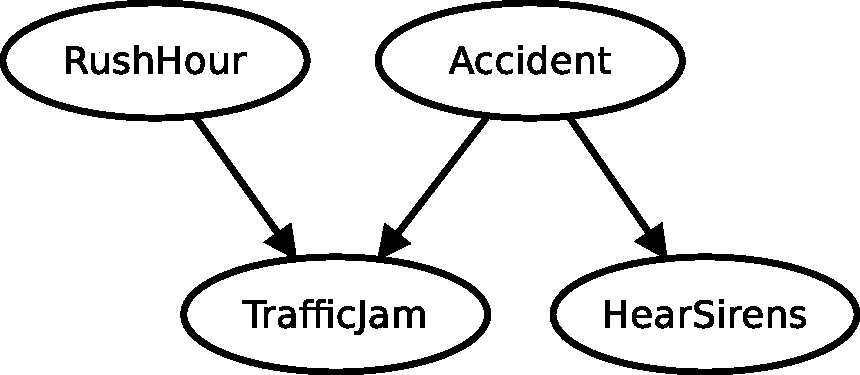
\includegraphics[scale=0.4]{fig/bn-d_sep-traffic}
        \caption{Example of an activated V-structure, $R\not\perp H \mid T$ (active trail $R-T-A-H$)}
        \label{fig:bn_d-separation_traffic}
    \end{subfigure}
  
    \begin{subfigure}[b]{0.42\linewidth}
        \vspace{0.5cm}
        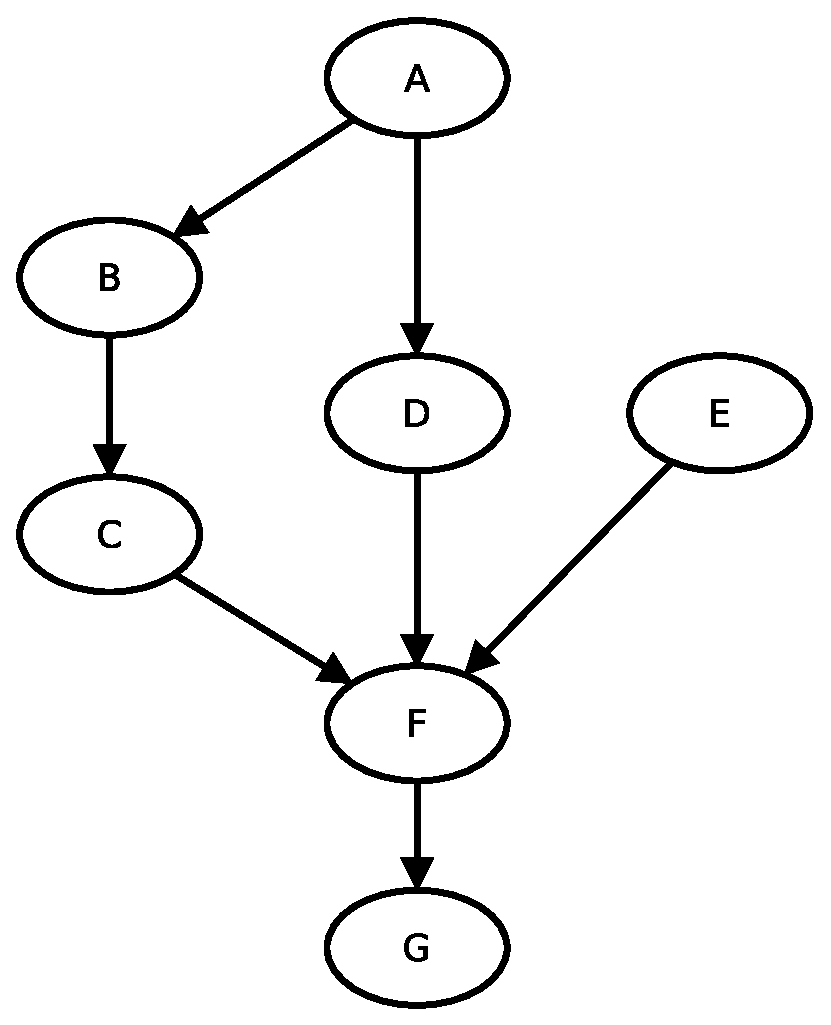
\includegraphics[scale=0.4]{fig/bn-d_sep-abstract}
        \caption{A more complicated network with multiple possible trails for some pairs of variables and other interesting features.}
        \label{fig:bn_d-separation_abstract}
    \end{subfigure}
    
    \caption{Networks for demonstration of d-separation and flow of influence.}
    \label{fig:bn_d-separation}
\end{figure}
\end{center}

It might be useful to explicitly point out what the notation $P(X \mid Parents(X))$ tells us in context of d-separation. It is a fact frequently used in mathematical derivations in context of BNs that, when given all parents $Parents(X)$ of a variable $X$, the variable is independent of all its indirect predecessors in the network. In Markov chain Monte-Carlo sampling we will also introduce so called \term{Markov blanket} of variable $X$ which is minimal set of variables such that $X$ is conditionally independent on any other variable in the network given its Markov blanket.













\section{Inference in Bayesian networks}
There are several types of queries that might be asked in context of a Bayesian network. In my case, inference in BNs is primarily understood as computing the posterior probability distribution for a set of query variables $\vars{X}$ given values $\vars{e}$ of evidence variables $\vars{E}$. Mathematically, the task is to compute the probability distribution $P(\vars{X} \mid \vars{e})$. Another type of query is so called \term{maximum a~posteriori} (abbreviated as MAP) which is finding $arg\ max_\vars{X} P(\vars{X} \mid \vars{e})$. MAP is basically used for finding out the most probable cause (concrete assignment of variables $\vars{X}$) for observation $\vars{e}$. A practical example could be getting the most probable word (sequence of letters) that corresponds to classifier output for a~segmented picture containing that word. Although, this is an example more frequently used in context of Markov networks.

Inference in a BN may be carried out in many ways depending on nature of the query and precision requirements. Exact inference is relatively straightforward in terms of mathematical description and naive algorithmic implementation but exhibits serious running-time disadvantage\,--\,exponential running time in the number of variables in the worst case. On the other hand, approximate inference methods allow us to answer queries more quickly but precision of the results may be questionable, especially for very rare events.


\subsection{Sum-product}
At the conceptual level, the simplest method for computing a conditional probability query is called sum-product. The problem at hand is to compute conditional probability distribution $P(\vars{X} \mid \vars{e})$ where $\vars{X}$ is one or more variables, $\vars{e}$ is an assignment to evidence variables $\vars{E}$ and $\vars{Y}$ are variables that are neither query nor evidence variables (the rest of the variables in the BN). The query is computed according to Bayes' theorem as follows:
\begin{equation*}
P(\vars{X} \mid \vars{e})
 = \frac{P(\vars{X}, \vars{e})} {P(\vars{e})}
 = \frac{\sum_\vars{Y} P(\vars{X}, \vars{y}, \vars{e})}{\sum_{\vars{X},\vars{Y}} P(\vars{x}, \vars{y}, \vars{e})}
\end{equation*}
The denominator is constant and since $P(\vars{X} \mid \vars{e})$ has to be a probability distribution, we can simply omit the denominator and in the end normalize numerator by an appropriate constant $\alpha$. Hence we can write:
\begin{equation*}
P(\vars{X} \mid \vars{e})
 = \alpha \sum_\vars{Y} P(\vars{X}, \vars{y}, \vars{e})
\end{equation*}
Computation of this expression using the sum-product method means performing four steps:
\begin{enumerate}
	\item reducing all factors in the Bayesian network by evidence $\vars{e}$,
	\item multiplying reduced factors all together producing single joint factor $P(\vars{X},\vars{Y},\vars{e})$ which is not a probability distribution because, in general, all values of the factor don't sum to one,
	\item marginalizing over the variables $\vars{Y}$ (non-query and non-evidence variables) and finally
	\item renormalizing the resulting factor, obtaining the probability distribution $P(\vars{X} \mid \vars{e})$.
\end{enumerate}

Every item of the sum in the numerator, ie. probability of every possible assignment to variables $\vars{Y}$, can be written, according to the joint probability distribution represented by a~BN (definition~\eqref{eq:bn_joint}), as a~product of conditional probabilities of all variables in given BN. This explains the name of this inference method\,--\,we effectively compute many products of conditional probabilities and sum over variables $\vars{Y}$.

Sum-product inference algorithm has, by its nature, exponential running time in the number of variables because it effectively generates the whole joint probability distribution encoded by a given Bayesian network and the size of a table representing any joint probability distribution has been earlier shown to be exponential in the number of variables. Because of this quality, the sum-product method is suitable only for inference in considerably small networks.



\subsection{Variable elimination}
Variable elimination algorithm can be seen as a somewhat smarter implementation of the sum-product algorithm explained above. Again, we answer the given query by multiplying all factors of the BN and summing out $\vars{Y}$ variables. The innovative ideas behind variable elimination are:
\begin{itemize}
	\item Suppose we sum over many variables in a product of factors, say one of these variables is $V$. Then factors whose scopes don't contain $V$ are irrelevant for the summation over~$V$ and hence these factors can be factored out in front of the summation over~$V$. This way we can push all summations \uv{as far to the right as possible}, so that each summation is ideally done only over product of factors containing the variable $V$ which is being summed out. What is the benefit for us? It can be shown~\cite{pgm} that running time of variable elimination depends on the size of the largest immediate factor during the summing-out process. When we sum only over product of factors containing variable $V$, the resulting immediate factor is the smallest possible. Because problem of determining the optimal order of elimination is NP-hard, greedy heuristics are usually used instead~\cite{pgm}.
	\item By definition of a conditional probability distribution it holds for any instantiation of parent variables that $\sum_V P(v \mid Parents(V)) = 1$. So, when computing posterior probability distribution $P(\vars{X} \mid \vars{e})$, any node (factor) $V$ that is not an ancestor of a~query or evidence variable can be omitted because, thanks to the order of elimination of variables, the term $\sum_V P(v \mid Parents(V))$ will be the rightmost summation (the innermost). So summing out $V$ is equivalent to totally excluding variable $V$ from the BN. Recursive implementation of this process could be done in the way of eliminating all leaf nodes that are not in $\vars{X} \cup \vars{E}$ and performing the same operation for as long as some node gets removed~\cite[p.~510]{russell_norvig_ed2}.
\end{itemize}

%\todo{řeči kolem, algoritmus, časová složitost, kliky}

Running time of the variable elimination algorithm in polytrees is $O(n)$~\cite[p.~510]{russell_norvig_ed2}, therefore it is a good method for answering individual queries $P(X \mid \vars{e})$ where $X$ is a single variable. Analogically, we can effectively compute probability distribution for small number of query variables $\vars{X}$ by computing individual distributions $P(X_i \mid \vars{e})$ for all $X_i \in \vars{X}$ and returning $P(\vars{X} \mid \vars{e}) = \prod_i P(X_i \mid \vars{e})$.

Running time in multiply connected networks is exponential in general but it can be coped with by clustering algorithms that transform multiply connected network into a~polytree which can be processed in linear time~\cite{russell_norvig_ed2}.


\subsection{Belief propagation}
Belief propagation~\cite{pgm} is an approximate inference algorithm from the family of so called \term{message passing algorithms}. The main idea is that nodes in the BN exchange information about their believes (probability distributions affected by evidence) and the whole network converges to some result close to true posterior probability. As methods from this family are far from trivial and they are not the aim of this thesis, we will not pay deeper attention to them.

\subsection{Sampling methods}
Monte Carlo methods (or particle methods) are stochastic methods of inference based on sampling the probability distribution induced by a BN. There are three main sampling methods: \term{direct sampling}, \term{rejection sampling} and \term{likelihood weighting}. All these methods basically generate a sufficient number of mutually independent samples and then compute simple statistics over these samples.

\subsubsection{Direct sampling}
Direct sampling is a method for computing probability distribution in the form $P(\vars{U} \mid \vars{V})$, ie. without any observed evidence. Of course must hold that $\vars{U} \neq \emptyset \wedge \vars{U} \cap \vars{V} = \emptyset$. For the sake of clarity of formulas we will consider $\vars{X} = \vars{U} \cup \vars{V}$ and compute the probability distribution $P(\vars{X})$ from which the conditional distribution $P(\vars{U} \mid \vars{V})$ can be easily obtained using Bayes' rule. This simplification is applied to all sampling methods further described. 

Direct sampling produces a number of samples, ie. of concrete events according to the probability distribution induced by the given BN, and then for every assignment $\vars{x}$ computes its probability as $P(\vars{x}) = N_\vars{x} / N$, where $N_\vars{x}$ is the number of samples in which variables $\vars{X}$ have the value $\vars{x}$ and $N$ is the number of all samples generated.

A single sample is generated as follows. First, randomly assign values to variables with no parents according to their probability distributions. Then choose a variable $V$ such that all of its parents have already been instantiated and randomly assign a value to $V$ according to the probability distribution $P(V \mid parents(V))$ where $parents(V)$ are the concrete values of the variables $Parents(V)$ in the current sample. Repeat this step until all variables have been instantiated, thereby obtaining a~sample. The process be done efficiently if we first compute topological sort of the BN and then sample variables in ascending order.

It can be shown~\cite[p.~491]{pgm} that to obtain an estimate with error bounded by $\epsilon$ with probability at least $1-\delta$ we need to generate $M$ samples:
\begin{equation*}%\label{eq:sampling_accuracy}
M \geq \frac{\ln(2 / \delta)}{2 \epsilon ^ 2}
\end{equation*}
Problem is that for a very unlikely event we may not generate a single sample and therefore the obtained probability distribution would indicate that this event is impossible (its probability equals to zero). Still, it would be a sound result within the error estimate $(\epsilon, \delta)$.

\subsubsection{Rejection sampling}
Direct sampling presented earlier doesn't allow for any evidence. Rejection sampling could be viewed as a simple extension of direct sampling for computing posterior probability distribution with evidence $\vars{E} = \vars{e}$, ie. distribution in the form $P(\vars{X} \mid \vars{e})$. The idea is to exclude samples inconsistent with evidence $\vars{e}$ meaning that when an evidence variable is instantiated during the production of a sample, the sample is discarded unless the randomly assigned value corresponds with the observed value in $\vars{e}$. The desired distribution is determined by computing $P(\vars{x} \mid \vars{e}) = N_{\vars{x}, \vars{e}} / N_\vars{e}$ for every instantiation of $\vars{X}$ where $N_\vars{e}$ basically is the number of all generated samples that haven't been discarded.

This simple approach bears the disadvantage that if the observed evidence is very unlikely then many samples get discarded and hence a lot of computational time is wasted because rejected samples don't contribute to the final probability distribution estimate. Unfortunately, when considering somewhat uniform distribution, the probability $P(\vars{e})$ decreases exponentially with the number of observed variables (eg. with symptoms of a~patient) and by the same rationale the number of samples that are not rejected decreases just as rapidly.

\subsubsection{Likelihood weighting}
Rejection sampling described earlier can theoretically be used for answering queries of the form $P(\vars{X} \mid \vars{e})$ but the number of rejected samples may be unbearable in practice. The likelihood weighting copes with this problem by forcing every sample to be consistent with observed evidence, ie. by artificially setting variables $\vars{E}$ to $\vars{e}$. Then, of course, not every sample is equally likely, so we cannot determine $P(\vars{x} \mid \vars{e})$ by simply dividing number of samples $N_{\vars{x},\vars{e}}$ by $N_\vars{e}$. For each sample we need some additional information which is the probability of assigning values $\vars{e}$ to evidence variables given values of other variables in the current sample~\cite[p.~514]{russell_norvig_ed2}. Let $\vars{Y}$ denote set of all variables in a BN other than the variables $\vars{X} \cup \vars{E}$. Then we can state that weight of a sample $\vars{x},\vars{e}, \vars{y}$ is $w_{\vars{x},\vars{e}, \vars{y}} = \prod_\vars{E} P(e \mid parents(E))$ where $parents(E_i)$ denotes assignment to variables $Parents(E_i)$ in the given sample $\vars{x},\vars{e}, \vars{y}$.

The algorithm of direct sampling needs to be changed in the following way. First of all, the counters of samples won't be integral but real as we don't count mere number of occurrences of a sample but its weighted number of occurrences. Also, when generating a~new sample we will keep not only the values of variables but also weight of the sample. When generating a new sample, first we set the weight of the current sample to 1. Then we sample all variables in topological order. For a non-evidence variable $X_i$ we proceed as in the case of direct sampling\,--\,randomly assign a value $x_i$ according to the probability distribution $P(X_i \mid parents(X_i))$ which is governed by the current instantiation of $X_i$'s parents. When we encounter an evidence variable $E_i$, we set it to value $e_i$ according to the given evidence $\vars{e}$ and multiply weight of the current sample by $P(e_i \mid parents(E_i))$. When a sample is completed we increase the counter $C_{\vars{x},\vars{e}}$ by the weight of the generated sample. The final probability distribution is computed for every $\vars{x} \in val(\vars{X})$ as follows:

\begin{equation}\label{eq:weighted_sampling}
    P(\vars{x} \mid \vars{e})
    = \frac{C_{\vars{x},\vars{e}}}{C_{\vars{e}}}
\end{equation}

Because the principle of weighted sampling might not be as obvious as in the cases of direct and rejection sampling I will try to elaborate and provide some insight. The key difference to previous sampling methods is that we want each sample to contribute to the final probability distribution estimate but then each generated sample cannot be accounted for by the same amount. Therefore the weight of a sample is used which literally bears the information how likely is the observed evidence $\vars{e}$ in that sample (for direct and rejection sampling the weight would be always one).
To understand weighted sampling better I have devised  a formal derivation of the formula~\eqref{eq:weighted_sampling}. Let $\vars{Y}$ denote set of all variables in a BN other than the variables $\vars{X} \cup \vars{E}$. First we will derive an alternative expression for $P(\vars{x}, \vars{e})$ which will be useful later.

\begin{eqnarray}
    P(\vars{x}, \vars{e})
    & = & \sum_\vars{Y} P(\vars{x}, \vars{e}, \vars{y}) \nonumber\\
    & = &
       \sum_\vars{Y} \Bigl( \prod_{E_i \in \vars{E}} P(e_i \mid parents(E_i)) \prod_{X_i \in \vars{X}} P(x_i \mid parents(X_i)) \prod_{Y_i \in \vars{Y}} P(y_i \mid parents(Y_i)) \Bigr) \nonumber\\
    & \approx &
       \sum_\vars{Y} \Bigl( w_{\vars{x},\vars{e},\vars{y}} \cdot \frac{N_{\vars{x},\vars{e},\vars{y}}}{N_{\vars{e},\vars{y}}} \cdot \prod_{Y_i \in \vars{Y}} P(y_i \mid parents(Y_i)) \Bigr) \nonumber\\
    & \approx &
       \sum_\vars{Y} \Bigl( w_{\vars{x},\vars{e},\vars{y}} \cdot \frac{N_{\vars{x},\vars{e},\vars{y}}}{N_{\vars{e}} \cdot \prod_{Y_i \in \vars{Y}} P(y_i \mid parents(Y_i))} \cdot \prod_{Y_i \in \vars{Y}} P(y_i \mid parents(Y_i)) \Bigr) \nonumber\\
    & = &
        \sum_\vars{Y} \Bigl( w_{\vars{x},\vars{e},\vars{y}} \cdot \frac{N_{\vars{x},\vars{e},\vars{y}}}{N_{\vars{e}}} \Bigr)
        = \frac{1}{N_\vars{e}} \cdot \sum_\vars{Y} \Bigl( w_{\vars{x},\vars{e},\vars{y}} \cdot N_{\vars{x},\vars{e},\vars{y}}\Bigr) \label{eq:weighted_sampling_P_x_e}
\end{eqnarray}

Let's go through the derivation step by step. The first line merely states we have to marginalize over all the remaining variables $\vars{Y}$ in the network.
On the second line we just rewrote the joint probability according to the definition of a~Bayesian network.
On the third line we replaced exact probabilities by their sampled equivalents (therefore the approximation symbol instead of equality). Namely, weight of the sample $w_{\vars{x},\vars{e},\vars{y}}$ is equal to the probability $P(\vars{e} \mid \vars{x},\vars{y})$ and ratio $N_{\vars{x},\vars{e},\vars{y}} / N_{\vars{e},\vars{y}}$ approximately equals to $P(\vars{x} \mid \vars{e},\vars{y})$.
On the forth line we needed to express the number $N_{\vars{e},\vars{y}}$ of samples with concrete values $\vars{e},\vars{y}$ using the probability $P(\vars{y} \mid \vars{x},\vars{e})$ and the total number of samples generated $N_\vars{e}$ (remember that in weighted sampling all samples are consistent with the evidence, so $N_\vars{e}$ really is the total number of samples).
Finally, on the fifth line the big products over $\vars{Y}$ cancel out and we obtain the final expression for $P(\vars{x},\vars{e})$.
Now let's make use of it:

\begin{eqnarray*}
    P(\vars{x} \mid \vars{e})
    & = &
      \frac
        {P(\vars{x},\vars{e})}
        {P(\vars{e})} = \frac{P(\vars{x},\vars{e})}{\sum_\vars{X} P(\vars{x},\vars{e})}
    = \frac
        {\frac{1}{N_\vars{e}} \cdot \sum_\vars{Y} \Bigl( w_{\vars{x},\vars{e},\vars{y}} \cdot N_{\vars{x},\vars{e},\vars{y}}\Bigr)}
        {\sum_\vars{X} \frac{1}{N_\vars{e}} \cdot \sum_\vars{Y} \Bigl( w_{\vars{x},\vars{e},\vars{y}} \cdot N_{\vars{x},\vars{e},\vars{y}}\Bigr)} \\
    & = &
      \frac
        {\sum_\vars{Y} \Bigl( w_{\vars{x},\vars{e},\vars{y}} \cdot N_{\vars{x},\vars{e},\vars{y}}\Bigr)}
        {\sum_\vars{X} \sum_\vars{Y} \Bigl( w_{\vars{x},\vars{e},\vars{y}} \cdot N_{\vars{x},\vars{e},\vars{y}}\Bigr)} \\
    & = & \frac{C_{\vars{x},\vars{e}}}{\sum_\vars{X} C_{\vars{x},\vars{e}}}
      = \frac{C_{\vars{x},\vars{e}}}{C_{\vars{e}}}
\end{eqnarray*}

On the first line we rewrote the conditional probability using Bayes' rule and then we substituted for $P(\vars{x},\vars{e})$ the expression~\eqref{eq:weighted_sampling_P_x_e} derived earlier.
On the second line the $1/N_\vars{e}$ cancel out.
To understand the third line we need to revisit how the weighted sampling works, especially what values are accumulated in a counter $C_{\vars{x},\vars{e}}$ and how. There are two key points. First, the weight $w_{\vars{x},\vars{e},\vars{y}}$ of each sample $\vars{x},\vars{e},\vars{y}$ is added to the counter $C_{\vars{x},\vars{e}}$ exactly $N_{\vars{x},\vars{e},\vars{y}}$-times. The second critical observation is that the counters don't care for values of the $\vars{Y}$ variables, so weights of two samples $\vars{x},\vars{e},\vars{y'}$ and $\vars{x},\vars{e},\vars{y''}$ are by the weighted sampling algorithm added to the same counter $C_{\vars{x},\vars{e}}$; this is effectively the same as marginalizing over the variables $\vars{Y}$ (ie. summing $\vars{Y}$ out) during the sampling.
  Combining these two pieces of information we conclude that the second and the third line have to equal. Formal derivation of the formula~\eqref{eq:weighted_sampling} for weighted sampling is now complete.

\medskip

I believe that the sampling process can furthermore be accelerated by omitting a set of variables, denoted $\vars{Z}$, from the network being sampled where $\vars{Z}$ is maximal set of variables satisfying the following two conditions: (1) $\vars{Z} \cap (\vars{X} \cup \vars{E}) = \emptyset$, (2) no direct or indirect child of any variable from $\vars{Z}$ is in $\vars{X} \cup \vars{E}$. Rationale behind this is the same as in the variable elimination algorithm\,--\,when computing the final probability distribution, we effectively sum out variables $\vars{Z}$ and it is irrelevant what random values they are assigned because if two samples differ only in the values of $\vars{Z}$ then these samples contribute to the same counter $C_{\vars{x},\vars{e}}$ by the same weight because $\vars{Z} \cap \vars{E} = \emptyset$. This observation is applicable to direct and rejection sampling as well.

Important drawback of likelihood weighting is that it doesn't account well for evidence in leaf nodes or near to them. This is because in that case we effectively sample the prior probability distribution and finally we modify weight of the generated sample by evidence but the sampling process is most of the time unaffected by the evidence and virtually only weights of samples take evidence into account. So, for a very rare instantiation of evidence variables (eg. for some rare and/or big set of medical symptoms) all of the generated samples might have very small weight and, in case of medical diagnosis, no sample representing the \uv{real cause} of observed evidence might actually get generated at all. Once again, this is because we sample prior probability distribution rather than posterior and these two distributions may be very different~\cite[p.~503]{pgm}.

\subsection{Markov Chain Monte Carlo}
The likelihood weighting method presented earlier doesn't account well for evidence near leaf nodes, ie. for so called \term{evidential reasoning}. Markov Chain Monte Carlo (MCMC) is also a stochastic method that generates samples but rather than generating each sample completely from scratch it modifies the last sample by resampling one of the non-evidence variables. This way, the information about all evidence variables propagates through the network and, with time, we get closer to the true posterior probability distribution $P(\vars{X} \mid \vars{e})$.

To explain how the MCMC algorithm works we first need to introduce so called \term{Markov blanket} of a~variable $X$ (also see Figure~\ref{fig:bn-markov-blanket}), denoted $MB(X)$. The Markov blanket of $X$ is the minimal set of variables not including $X$ such that $X$ is conditionally independent of all other variables in the BN given $MB(X)$. It is fairly obvious that the Markov blanket includes variables $Parents(X)$ and direct children of $X$, denoted $Children(X)$, because there is a direct connection between these variables and $X$. Furthermore, $MB(X)$ also needs to include parents of every variable in $Children(X)$ because observing any of the children $C_i \in Children(X)$ activates a V-structure and $X$ becomes conditionally dependent on $Parents(C_i)$ given $C_i$. Formally the Markov blanket could be defined as follows:
\begin{equation*}
MB(X) = Parents(X) \cup Children(X) \cup \!\!\!\!\!\!\!\! \bigcup_{C_i \in Children(X)} \!\!\!\!\!\!\!\!\!\!\!\! Parents(C_i) \setminus \lbrace X \rbrace
\end{equation*}

\begin{figure}[h]
    \centering
    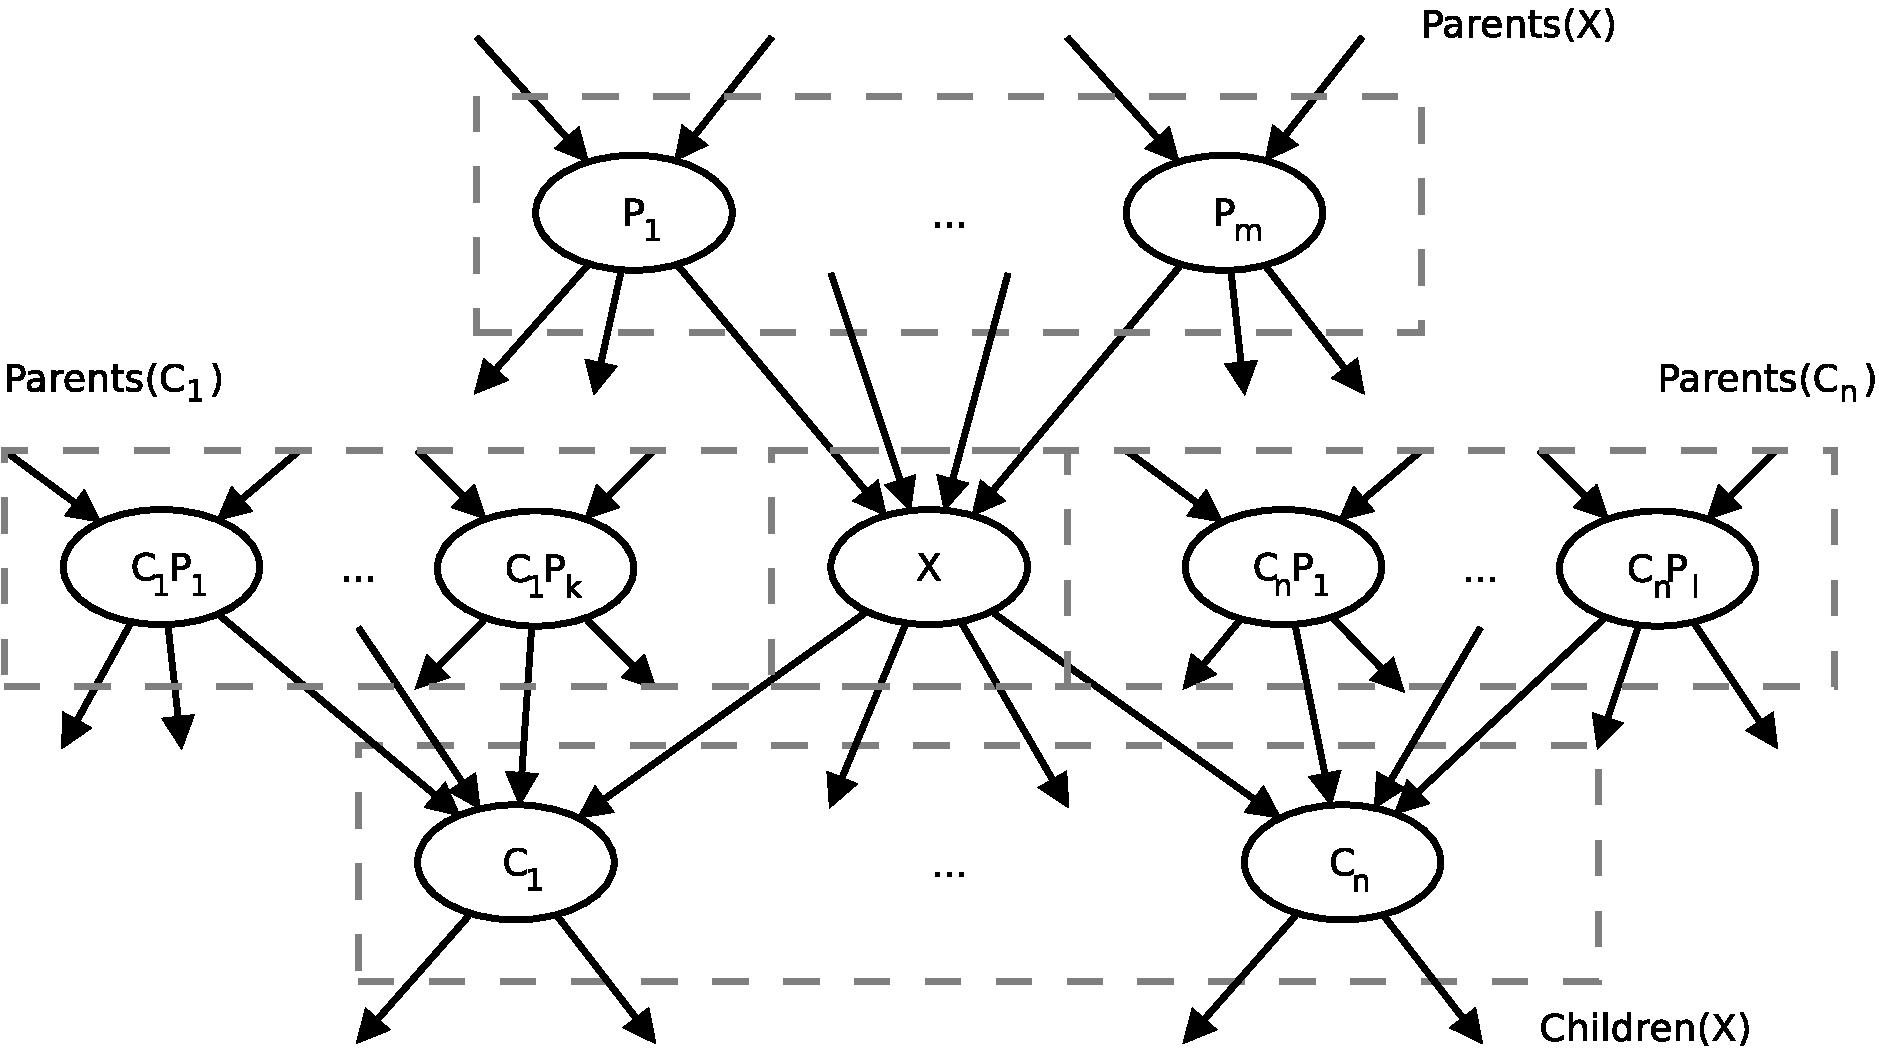
\includegraphics[scale=0.39]{fig/bn-markov_blanket}
    \caption{Markov blanket $MB(X)$ of variable $X$ is the set of all variables in this figure except for $X$.}
    \label{fig:bn-markov-blanket}
\end{figure}

Now, in order to resample some non-evidence variable $X$ and thereby to produce a new MCMC sample, we need to compute the probability distribution $P(X \mid mb(X))$ and sample new value of $X$ from this distribution. In a sense, Markov blanket of variable $X$ defines context of the resampling, ie. all the variables whose values we need to know.

The MCMC algorithm~\cite[p.~516]{russell_norvig_ed2} starts by producing one sample consistent with the evidence, eg. by one iteration of likelihood weighting with the weight discarded. Then we repeat the following: For each non-evidence variable $V$ we resample this variable from the current distribution $P(V \mid mb(V))$ producing a new sample with value of variable $V$ potentially changed. For the new sample we increase the corresponding counter $N_{\vars{x},\vars{e}}$ and proceed with resampling of another variable. The distribution $P(V \mid mb(V))$ needed for resampling of variable $V$ can be obtained by computing $P(v \mid mb(V))$ for every $v$ as follows:
\begin{equation*}
    P(v \mid mb(V)) = \alpha \cdot P(v \mid parents(V)) \!\!\!\!\!\!\!\! \prod_{C_i \in Children(V)} \!\!\!\!\!\!\!\!\!\!\!\! P(c_i \mid parents(C_i))
\end{equation*}
where $\alpha$ is a normalizing constant. Note that $mb(\cdot)$ and $parents(\cdot)$ denote concrete instantiation of variables $MB(\cdot)$ and $Parents(\cdot)$ in the current sample. As we can see, when computing the probability distribution $P(V \mid mb(V))$ we only need to account for probabilities of variables $V$ and $Children(X)$, not of the whole Markov blanket. This is because when we set $V$ to concrete value $v$, only probabilities in nodes $\lbrace V \rbrace \cup Children(X)$ are affected due to the definition of a Bayesian network where probability at a node depends purely on its parents.

Intuition behind the MCMC algorithm is that the sampling process will reach a dynamic equilibrium in which time spent with each instantiation of non-evidence variables (ie. the counter of samples $N_{\vars{x},\vars{e}}$) is proportional to the probability of this instantiation. More formally, MCMC is based on state space induced by a BN represented by a Markov model~\cite[p.~516]{russell_norvig_ed2} but this theory is not necessary for understanding the MCMC inference method.

%\note{pgm 541+ has good notes of other papers} % SP

\begin{comment}
$\pi(x)$ is the stationary distribution (ustálený)

works for regular Markov chains ($\exists k \forall x, x':$ z $x$ do $x'$ se lze dostatat přesně v $k$ krocích s nenulovou pstí)
\end{comment}












\section{Model learning}
So far, we have been reasoning about Bayesian networks that were already given to us, so that both the structure of the BN and the CPDs associated with nodes were known. Now we are going to examine the problem of creating a Bayesian network so that the probability distribution it induces somehow corresponds to the real probability distribution of the target domain.

Basically, there are two approaches to creating a BN. First option is to cooperate with an expert of the target domain who can make correct dependency and independency assumptions and provide us with conditional probability distributions, ie. with CPDs for all the nodes. The other approach is to use some fully automated techniques for creating models based on a sufficiently big dataset. The dataset can be viewed as a set of samples of the target probability distribution $P*$ which we attempt to reconstruct. The aim is to create a model $\tilde{\mathcal{M}}$ such that the probability distribution $P_{\tilde{\mathcal{M}}}$ induced by $\tilde{\mathcal{M}}$ is very close to the original distribution $P*$.

Complete construction of a BN through cooperation with an expert is problematic because, for a non-trivial BN, the task often requires significant time (several months~\cite{pgm}), the expert might not correctly capture CPDs, especially for nodes with large number of parents, and furthermore there might not even be an expert of the target domain at all. On the other hand, automated techniques of model construction are constrained by limited computational power and, more importantly, by the size of the supplied dataset. As will be shown later, we encounter classical problem of overfitting and bias-variance trade-off present in the whole field of artificial intelligence and machine learning. In practice, these two approaches are often combined in the way that an expert defines structure (all variables and their dependencies) and an automated process determines CPDs from a supplied dataset.

%\todo{maybe include general metrics?} % SP

\section{Parameter estimation}
Goal of parameter estimation methods is to supply CPDs to a BN whose structure is already known. For the estimation to be reasonably correct, we need to have sufficiently large dataset wrt. complexity of the BN structure.


\subsection{Maximum likelihood estimation}
Maximum likelihood estimation views the dataset $\mathcal{D}$ as a set of independent samples $x_1, \dots, x_m$ obtained from a~parametrized probability distribution with parameter $\Theta$. The parameter $\Theta$ can be seen as a vector of entries of all CPDs in the given BN (roughly speaking, $\Theta$ is \uv{serialized} equivalent of tabular CPDs). Core of the maximum likelihood estimation is to choose $\Theta$ in such a way that the probability of obtaining samples $x_1, \dots, x_m$ from the parametrized distribution is maximal. Formally $\Theta = \arg \max P(\mathcal{D} \mid \Theta)$ where $P(\mathcal{D} \mid \Theta)$ is called the \term{likelihood function}.

Let's inspect a simple example of $m$ coin tosses $x_1, \dots, x_m$ with a biased coin (inspired by~\cite{pgm}) for which $P(X = heads) = \theta$. Let's suppose we get $H$ times heads and $T$ times tails. Then we can write $P(x_1,\dots,x_m \mid \theta) = \theta^H (1 - \theta)^T$ because the coin tosses are mutually independent given $\theta$. The task of maximizing the expression $\theta^H (1 - \theta)^T$ is equivalent to maximizing its logarithm $H \cdot \ln(\theta) + T \cdot \ln(1 - \theta)$. The equation $\frac{\partial}{\partial\theta} \bigl( H \cdot \ln(\theta) + T \cdot \ln(1 - \theta) \bigr) = 0$ yields global maximum at $\theta = H / (H + T)$ which is a fairly intuitive conclusion\,--\,probability of heads is, according to the experiments, computed as the number of times we got heads divided by the number of all tosses. So, maximum likelihood estimation is the approach we would normally apply, probably without even knowing its proper justification. Similar formulas as for the binomial variable can be obtained for a~general set $\vars{X}$ of multinomial variables, formally $P(\vars{X}=\vars{x}) = N_\vars{X} / N_{all}$.

Now suppose we want to compute probability distribution $P(X \mid Parents(X))$ for some node $X$ according to our dataset, ie. to compute the CPD for that node. Maximum likelihood estimation is, as demonstrated earlier, an intuitive approach when we partition the dataset into disjoint subsets, each for a concrete instantiation of variables $\lbrace X \rbrace \cup Parents(X)$. Operating just with cardinalities of these subsets, a CPD entry $P(X=x_i \mid Parents(X) = \vars{p_j})$ is computed as the ratio $N_{x_i,\vars{p_j}} / N_{\vars{p_j}}$. Potential problem with this approach is that the number of subsets grows exponentially with the number of parents and hence the estimated CPD looses precision. This exponential explosion of possible instantiations is called \term{fragmentation} and is one of the main problems of learning BNs from data. Because of fragmentation, a perfect model (in terms of structure) capturing all real dependencies among variables might be outperformed by a simpler (and thereby wrong) model just because the amount of data is insufficient to compute CPDs for the more complicated structure accurately\footnote{Such observation has often been made, for example, with the Naïve Bayes model which assumes that any two effect variables are independent given the cause variables. Such assumption is seldom justified, nevertheless Naïve Bayes models have proved themselves to perform well.}~\cite{pgm}. This is a~typical AI problem of overfitting. In extreme cases, $N_{x_i,\vars{p_j}}$ could even be zero which is usually very wrong because, according to computed CPDs, there could never be an event in which $X_i = x_i$ and $Parents(X_i) = \vars{p_j}$. This can be prevented by applying the Laplace's correction commonly used in context of Naïve Bayes classifier.


\subsection{Bayesian estimation}
An important drawback of the maximum likelihood estimation presented earlier is that it doesn't really account for the size of the dataset\,--\,small dataset may not have enough samples for every instantiation of every variable and its parents and the dataset might also be noisy. The key idea of Bayesian estimation is to view the parameters $\Theta$ themselves (ie. CPDs) as random variables with some prior distribution $P(\Theta)$ and then, according to the supplied dataset, compute the posterior distribution $P(\Theta \mid \mathcal{D})$ which will be our estimated CPDs. So, parameter learning could in this case be viewed as a type of inference.
More formally, we define a~prior distribution $P(\Theta)$ over parameters $\Theta$ with some degree of strength of this initial distribution (will be explained later) and then, using the Bayes' rule, compute the posterior probability distribution $P(\Theta \mid \mathcal{D}) \propto P(\mathcal{D},\Theta) P(\Theta)$ as we get more empirical data; the posterior distribution corresponds to the network parameters determined by the Bayesian estimation method.

From its nature, Bayesian estimation can capture prior believes regarding the CPDs. For example, in case of a die the general expectation is that the probability of rolling a~chosen number is $1/6$. Now, when inferring parameters $\Theta$ for a die, Bayesian estimation can distinguish between rolling a~six three times out of twelve throws, which may be accounted merely to statistical noise, and rolling a six 3\,000 times out of 12\,000 throws. It is clear that these two datasets tell us something different about the die, although probability of rolling a six, according to the maximum likelihood estimation discussed earlier, is $1/4$ in both cases\,--\,ratio $N_6 / N_{all} = 3/12 = 3\,000/12\,000$. With Bayesian estimation the inferred probability of rolling a six will still be close to the generally expected $1/6$ when working with just twelve samples. On the other hand, in the situation with 12\,000 samples the inferred probability of rolling a six will be much closer to $1/4$. Another example of shortcomings of the maximum likelihood estimation could be an insurance company attempting to evaluate driving skills of a brand new young driver. If this driver were to crash on his very first ride, certainly he shouldn't get a good rating but it would be unreasonable to conclude that probability of him crashing the next day is $1/1 = 100 \%$ as suggested by the maximum likelihood estimation.

In context of Bayesian estimation, besides the real dataset $\mathcal{D}$ containing real samples, we also work with imaginary \term{pseudo-samples}. These pseudo-samples define the prior distribution $P(\Theta)$ by plain maximum likelihood estimation as a ration of pseudo-sample counts\,--\,for example, in the prior distribution $P(\Theta)$ holds that $P(X = x) = \alpha_x / \alpha$ where the $\alpha$ symbol, optionally with a subscript, is a~counter of pseudo-samples similar to $N$ counters of real samples introduced earlier. The exact mathematical derivation~\cite[p.~733]{pgm} of formulas for Bayesian estimation is based on \term{Dirichlet distribution} with hyperpameters $(\alpha_1,\dots,\alpha_k)$ that correspond to the pseudo-sample counters. The derivation is not trivial and also is not needed further in this thesis, so we jump straight to the practical conclusions and interpretations. Bottom line is that for a multinomial variable the Dirichlet distribution has the nice property that the prior distribution $P(\Theta)$ and the posterior $P(\Theta \mid \mathcal{D})$ have exactly the same form as a ratio of some counters, so when the prior distribution is computed by maximum likelihood estimation over a set of pseudo-samples using $\alpha$ counters, then posterior distribution is computed also using maximum likelihood estimation but over dataset containing both real samples and pseudo-samples as well, ie. involving both $\alpha$ and $N$ counters. For a~given dataset $\mathcal{D}$ and some vector of hyperparameters $\vec{\alpha}$ the probability of variable $X$ having value $x_i$ is given as follows (for a node without and with parents respectively):

\begin{equation*}
    \begin{array}{rcl}
    P(X = x_i \mid \mathcal{D}) &
     = &
     \displaystyle\frac
        {\alpha_{x_i} + N_{x_i}}
        {\sum_j (\alpha_{x_j} + N_{x_j})}\\
        & & \\
    P(X = x_i \mid Parents(X) = \vars{p_i}, \mathcal{D}) &
     = &
     \displaystyle\frac
        {\alpha_{x_i, \vars{p_i}} + N_{x_i, \vars{p_i}}}
        {\sum_j (\alpha_{x_j, \vars{p_i}} + N_{x_j, \vars{p_i}})}
    \end{array}
\end{equation*}

Let's take a closer look at the hyperparameters. It is easy to see from the formulas above that the relative difference between $\alpha$ and $N$ terms determines strength of the prior distribution $P(\Theta)$, ie. how many real samples accounted for in the $N$ counters does it take to significantly deviate from the prior distribution governed purely by hyperparameters $\alpha$.
We have already encountered two special cases of hyperparameters\,--\,$(0,\dots,0)$ is the pure maximum likelihood estimation when we compute the CPDs based just on the dataset $\mathcal{D}$; hyperparameters $(1,\dots,1)$ correspond the maximum likelihood estimation with Laplace's correction.
It is clear that the maximum likelihood estimation and the Bayesian estimation are asymptotically the same for large datasets. However, Bayesian estimation generalizes better with sparse datasets and exhibits lower sensitivity to noise in the data~\cite[p.~749]{pgm}. In addition, we can quite simply enforce that each possible instantiation of variables in a~network occurs with non-zero probability.

At this point the only thing we haven't covered yet is how can the hyperparameters be defined in a readable and easy-to-understand fashion. There will be two approaches, both working with so called \term{equivalent sample size} $\alpha$ which can be viewed as the total number of pseudo-samples. First, and more general, option is to use another BN whose CPD entries define the prior distribution $P(\Theta)$ and equivalent sample size determines strength of the prior. Structure of this BN is identical to the BN, whose CPDs we want to estimate, therefore it is easy to specify the prior distribution simply by filling in prior CPD entries. Hyperparameters are then determined using inference (eg. by sampling) of that BN as $\alpha_{x_i,\vars{p_j}} = \alpha \cdot P(x_i, \vars{p_j})$. Second approach is to use \term{uniform prior} in which each event is equally likely, ie. $P\bigl(X = x_i, Parents(X) = \vars{p_j}\bigr) = \alpha / card\bigl(\lbrace X \rbrace \cup Parents(X)\bigr)$ where $card(\cdot)$ denotes the number of all possible instantiations of the specified set of variables.

\medskip

Parameter learning methods explained so far deal strictly with table CPDs and assume that parameters $\Theta$ of the BN are independent given complete data. Advanced methods of parameters learning include learning structured probability distributions (eg. tree-structured CPDs) and dependent or shared parameters~\cite{pgm}.












\section{Structure learning}
So far we have seen how to compute CPDs for a given graph structure of a BN based on some dataset. Learning the structure itself can be useful for a number of reasons. For example, we might want to create an accurate model of certain domain to be able to perform inference later (eg. medical diagnosis or prediction of traffic conditions~\cite{horvitz05}). Other application could be in the field of knowledge discovery when we are interested in finding out the causal dependencies between random variables so finding the structure itself is our goal (eg. discovering protein-signaling networks purely based on statistical data~\cite{sachs05}).

Learning structure of a BN is a complicated task. One of the problems is to pick a~good trade-off between high bias (restricting complexity of the graph structure) and high variance (allowing more dependencies to get a better fit for training data with the cost of higher fragmentation). As we have already discussed, with a small dataset we may actually benefit by having a simpler structure. On the other hand, with a large dataset we don't want to restrict our hypothesis space too much because the dataset is sufficient to learn higher number of parameters with reasonable accuracy.

In this thesis we are going to focus on \term{score-based} methods of structure learning, concretely likelihood score and Bayesian score. In the case of score-based methods, structure learning is basically a discrete optimization task and for such tasks there are many well known approaches\,--\,greedy search, simulated annealing, genetic algorithms etc. Nevertheless, in the field of learning Bayesian networks the majority of structure learning methods are local state-space search algorithms~\cite[p.~814]{pgm} (eg. hill climbing, greedy search, tabu search). A~common requirement for using any optimization technique is a mechanism that evaluates quality of a candidate solution. Such role is carried out by the scoring functions which we will discuss in detail.

Other than the score-based approach there are also constraint-based approaches~\cite[p.~786]{pgm} which make a series of one-time decisions regarding dependency and independency of variables (eg. by performing independency tests using $\chi^2$) and construct a model satisfying those assumptions. The fact that decisions are irreversible, as opposed to score-based methods, makes the constraint-based approach somewhat limited.


\subsection{Optimization algorithm}
As we have already discussed, in context of Bayesian networks, the techniques most frequently used are local state-space search methods. We will use the tabu-search algorithm~\cite[p.~816]{pgm} which is an extension of simple hill climbing and works as follows. We have an initial graph structure with fixed set of variables. The initial structure may be empty, it may be the best-scoring tree/forest or some network capturing our prior knowledge and believes regarding the target domain. At each iteration we evaluate the change of score for all possibilities of adding a new edge, reversing direction or deleting an existing edge in the current structure and we accept the structural modification with the best score gain. Those actions are repeated until the solution improves. Furthermore, we maintain a list of last $n$ structural modifications (a \term{tabu-list}) and disallow those modifications to be reversed. If we hit a local optima, ie. no feasible structural modification leads to a better score, we make a~predefined number of random steps (called \term{random restart}) and continue the local search.



\subsection{Likelihood score}
The likelihood score has information-theoretic foundations and basically quantifies how well a given network structure matches our dataset. We assume that for a given structure $\mathcal{G}$ the parameters $\Theta$ are learnt using the maximum likelihood estimation, so the likelihood score really evaluates the hypothesis as a complete BN $(\mathcal{G}, \Theta)$, only the parameters are implicit.

Let's suppose we have a dataset $\mathcal{D} = \lbrace \xi^{(1)}, \dots, \xi^{(m)} \rbrace$. Again, learning corresponds with maximizing probability of sampling exactly the data $\mathcal{D}$ from the learnt network, only now we search for optimal BN structure rather than parameters. Concretely, we will focus on maximizing the likelihood function $P(\mathcal{D} \mid \Theta, \mathcal{G})$ which is basically probability of obtaining exactly the samples contained in dataset $\mathcal{D}$ from the network $(\mathcal{G},\Theta)$, ie. one can write $P(\mathcal{D} \mid \Theta, \mathcal{G}) = P(\xi^{(1)} \mid \Theta, \mathcal{G}) \dotsm P(\xi^{(m)} \mid \Theta, \mathcal{G})$. Furthermore, we will use \term{log-likelihood function} $\log P(\mathcal{D} \mid \Theta, \mathcal{G})$. This is a useful trick because logarithm transforms a product into a sum which allows us to compute score of a network based purely on computations over individual nodes as we will see later (the likelihood score decomposes over a network).

To understand how the likelihood score changes for two networks that differ only by presence of a~single edge, we will examine network $\mathcal{G}_1$ with two independent variables $X$ and $Y$ and network $\mathcal{G}_2$ with structure $X \rightarrow Y$. From the previous text we know likelihood scores of these networks (logarithms of likelihood functions) can be computed as follows:
\begin{eqnarray*}
    score_L(\mathcal{G}_1 : \mathcal{D}) & = & \sum_{i=1}^{|\mathcal{D}|} \Bigl(\log \hat P(x^{(i)}) + \log \hat P(y^{(i)})\Bigr)\\
    score_L(\mathcal{G}_2 : \mathcal{D}) & = & \sum_{i=1}^{|\mathcal{D}|} \Bigl(\log \hat P(x^{(i)}) + \log \hat P(y^{(i)} \mid x^{(i)})\Bigr)
\end{eqnarray*}
where $score_L(\mathcal{G}_1 : \mathcal{D})$ denotes the likelihood score of dataset $\mathcal{D}$ in network with structure $\mathcal{G}_1$, $x^{(i)}$ is value of variable $X$ in sample $\xi^{(i)}$ and $\hat P$ denotes so called \term{empirical distribution}. Empirical distribution is computed from the dataset $\mathcal{D}$ according to the maximum likelihood principle (eg. $\hat P(x_i) = N_{x_i} / N$ or $\hat P(x_i \mid y_j) = N_{x_i,y_j} / N_{y_j}$) and therefore $\hat{P}(\cdot)$ also corresponds to the CPD entries (we have said that parameters $\Theta$ of a network with given structure are assumed to be computed using maximum likelihood estimation).

Now let's examine the difference between having an edge between variables $X$ and $Y$ or not, how does the likelihood score change? We obtain the following result (derivation inspired by~\cite[p.~791]{pgm}):
\begin{eqnarray*}
   score_L(\mathcal{G}_2 : \mathcal{D}) - score_L(\mathcal{G}_1 : \mathcal{D}) 
     & = & \sum_{i=1}^{|\mathcal{D}|} \log \hat P(y^{(i)} \mid x^{(i)}) - \sum_{i=1}^{|\mathcal{D}|} \log \hat P(y^{(i)}) \\
     & = & \sum_{X,Y} N_{x,y} \log \hat P(y \mid x) - \sum_{Y} N_y \log \hat P(y) \\
     & = & \sum_{X,Y} N \cdot \hat P(x,y) \log \hat P(y \mid x) - \sum_{Y} N \cdot \hat P(y) \log \hat P(y) \\
     & = & \sum_{X,Y} N \cdot \hat P(x,y) \log \hat P(y \mid x) - \sum_{X, Y} N \cdot \hat P(x, y) \log \hat P(y) \\
     & = & N \sum_{X,Y} \hat P(x,y) \log \frac{\hat P(y \mid x)}{\hat P(y)}
       =   N \sum_{X,Y} \hat P(x,y) \log \frac{\hat P(x, y)}{\hat P(x) \hat P(y)} \\
     & = & N \cdot I_{\hat P}(X; Y)
\end{eqnarray*}
First, I will explain the derivation step by step and the next paragraph will address the question of usefulness of the derived result. The first step (performed on the second line) is to change the logic of the summation from \uv{over the dataset $\xi^{(1)},\dots,\xi^{(m)}$} to \uv{over possible instantiations of $X,Y$}; such change is legal because each $\hat P(\cdot)$ value will be taken into account just as many times as before.
On the third line the counts $N_{x,y}$ and $N_y$ are expresses using size of the dataset $N$ and empirical probabilities of respective instantiations $x,y$ and $y$.
After that, on the fourth line, we can extend the second summation from just over $Y$ to over $X,Y$.
The last step, the fifth line, is merging the two sums and logarithms and applying Bayes' rule on the $\hat P(y \mid x)$ term. Finally, we introduce special notation for the final expression.

The term $I_{\hat P}(X; Y)$ is called \term{mutual information} between variables $X$ and $Y$ in the distribution $\hat P$ and expresses the average distance between the joint distribution $\hat P(X,Y)$, in which the variables may be dependent, to the distribution given as product of marginal distributions $\hat P(X)$ and $\hat P(Y)$, when the variables are independent. The bigger the distance the more variables $X$ and $Y$ are correlated which in context of a BN means they should be connected by an edge. So, mutual information is a natural way of measuring strength of dependency among variables. In a similar fashion mutual information is defined for sets of variables $\vars{X},\vars{Y}$ rather than for single variables $X,Y$, we just sum over all possible instantiations $\vars{x},\vars{y}$ of $\vars{X},\vars{Y}$. It can be shown (for details see~\cite[p.~792]{pgm}) that the overall likelihood score decomposes over a~BN with general structure $\mathcal{G}$ as follows:
\begin{equation}
    score_L(\mathcal{G} : \mathcal{D}) = N \!\!\!\!\!\! \sum_{X_i \in Nodes} \!\!\!\!\!\! I_{\hat P}(X_i;Parents(X_i)) - N \!\!\!\!\!\! \sum_{X_i \in Nodes} \!\!\!\!\!\! H_{\hat P}(X_i)
\end{equation}
where $H_{\hat P}(\cdot)$ is entropy of an individual variable in the distribution $\hat P$. As we can see, $H_{\hat P}(\cdot)$ is a constant relative to the structure $\mathcal{G}$. So, in order to compare two network structures by their likelihood scores we only need to consider value of the sum  over the mutual information terms and computation of the $H_{\hat P}(\cdot)$ may be ommited.

\medskip
The difference of likelihood scores between a superstructure with more edges and its substructure is always non-negative and, in fact, is equal to zero if and only if the two variables $X,Y$ in the dataset $\mathcal{D}$ appear to be \emph{perfectly independent} which is due to statistical noise almost never true. Therefore the likelihood score itself almost always suggests the greedy heuristics to add an edge which would eventually lead to a very densely connected network. In other words, the likelihood score is very prone to overfitting. This problem can be addressed by thresholding of the score increase or by restraining complexity of the network (defining maximal number of parents or maximal number of overall network parameters). Another approach is to account for network complexity in the scoring function itself, thus imposing a penalty on complicated structures. The latter is exactly what the BIC score does.



\subsection{BIC score}
The likelihood score discussed earlier never favors a simpler structure over a more complex one. We will discuss a variant of Bayesian score called \term{BIC score} which is, in the end, just the likelihood score extended by a penalty term although theoretical foundations and mathematical derivations leading to the final formulas are entirely different.

%\note{pgm 798 gives nice understanding of the use of gamma function}

The BIC score takes into account both network complexity as well as the size of the dataset and combines these two pieces of information in such a way that with a small dataset the BIC score tends to keep the structure simple and allows only for the strongest dependencies to be be reflected in the network. As the dataset gets larger, the BIC score allows for a more complicated structure that encodes also weaker dependencies indicated by the data.

The BIC score is defined as follows (for complete derivation see~\cite[p.~794]{pgm}):
\begin{equation}\label{eq:bic_score}
    score_{BIC}(\mathcal{G} : \mathcal{D}) = N \!\!\!\!\!\! \sum_{X_i \in Nodes} \!\!\!\!\!\! I_{\hat P}(X_i;Parents(X_i)) - N \!\!\!\!\!\! \sum_{X_i \in Nodes} \!\!\!\!\!\! H_{\hat P}(X_i) - \frac{\log N}{2} Dim[\mathcal{G}]
\end{equation}
where $Dim[\mathcal{G}]$ is dimension of the network (number of its parameters). Notice that the two sums are the likelihood score $score_{L}(\mathcal{G} : \mathcal{D})$. We can see that the BIC score increases linearly in $N$ with variables, that appear to be dependent, being connected (the first term) and decreases logarithmically in $N$ with the network complexity (the third term). Thus for a sparse dataset only the strongest dependencies will be reflected in the final network, whereas for a~large dataset the penalization grows at slower rate allowing the network to have a~more complicated structure including also weaker dependencies.

Note that the BIC score decomposes over the graph $\mathcal{G}$, so when we want to evaluate some structural change, we only need to consider the score difference of nodes affected by this change, so called \term{delta score}. This observation is crucial for an effective implementation of structure learning based on local optimization of the score function. 



\subsection{Bayesian score}
Bayesian score for a graph structure is yet another application of the Bayesian principle which we have already encountered in context of parameter estimation\,--\,whatever we are uncertain about should be modeled as a random variable. In case of Bayesian score we are uncertain both about parameters $\Theta$ (as in Bayesian parameter estimation) and even about the network structure $\mathcal{G}$. To state the idea formally, graph structure $\mathcal{G}$ is a~random variable for which holds $P(\mathcal{G} \mid \mathcal{D}) = P(\mathcal{D} \mid \mathcal{G}) P(\mathcal{G}) / P(\mathcal{D})$. The denominator is independent of the network structure and parameters, so we can safely consider just the numerator. Further we will consider logarithm of the numerator which is perfectly legal for a scoring function because logarithm is a~monotone function and probability is always non-negative. By applying logarithm to the numerator we obtain the Bayesian score for structure $\mathcal{G}$ and data $\mathcal{D}$ as:
\begin{equation}\label{eq:bayesian_score_general}
    score_B(\mathcal{G} : \mathcal{D}) = \log P(\mathcal{D} \mid \mathcal{G}) + \log P(\mathcal{G})
\end{equation}
The structure prior $P(\mathcal{G})$ in the equation~\eqref{eq:bayesian_score_general} allows us to penalize certain structures. However, effect of the structure prior is rather minor, especially in asymptotic analysis~\cite[p.~804]{pgm}, because this term doesn't change with the number of samples. Literature suggests using a uniform prior or a prior that exponentially penalizes complexity of the structure which is useful for sparse datasets~\cite{pgm}.

The term $P(\mathcal{D} \mid \mathcal{G})$ in equation~\eqref{eq:bayesian_score_general} will be our major concern. It is a marginal distribution (because all possible parameter settings $\Theta$ are marginalized out) mathematically defined in the following integral form:
\begin{equation}\label{eq:bayesian_score_marginal}
    P(\mathcal{D} \mid \mathcal{G})
    =
    \int_{\Theta} P(\Theta \mid \mathcal{G}) P(\mathcal{D} \mid \mathcal{G}, \Theta) \ d \Theta
\end{equation}
The integral expression can be interpreted as computing the average probability of $\mathcal{D}$ given $\mathcal{G},\Theta$ weighted by probabilities of all possible parameter settings $P(\Theta \mid \mathcal{G})$. So, the Bayesian estimation is less optimistic when determining probability of a dataset given structure. On the other hand, the BIC score considers only single parameter setting $\Theta$ computed by the maximum likelihood estimation which is \uv{tailored} for the specific dataset to maximize probability of the data given structure. Therefore Bayesian score is less prone to overfitting~\cite[p.~795]{pgm}.
The integral expression~\eqref{eq:bayesian_score_marginal} is hard to deal with practically. Fortunately, for a~BN with multinomial variables, whose prior parameter distribution is a Dirichlet distribution with hyperparameters $(\alpha_1, \dots, \alpha_n)$, the expression $P(\mathcal{D} \mid \mathcal{G})$ can be written using the chain rule as follows:
\begin{equation}\label{eq:bayesian_score_chain_rule}
    P(\mathcal{D} \mid \mathcal{G})
    =
     \prod_{i = 1}^{| \mathcal{D} |}
             P \Bigl( \xi^{(i)} \mid \mathcal{G}, \xi^{(1)}, \dots, \xi^{(i - 1)} \Bigr)
\end{equation}
where $\mathcal{D} = \lbrace \xi^{(1)}, \dots, \xi^{(m)} \rbrace$ is a dataset. If you think about the equation~\eqref{eq:bayesian_score_chain_rule}, we could view each of the product terms as making a prediction of how likely is the data instance $\xi^{(i)}$ given the previous instances and the structure $\mathcal{G}$, ie. as if we were predicting probability of an unseen instance $\xi^{(i)}$ based on a model learnt using the previous instances. In other words, we measure predictive power the network structure for the whole dataset, only without making any explicit testing or validation.

Before we get to the general expression for $P(\mathcal{D} \mid \mathcal{G})$ in context of Bayesian networks let's consider a simple coin flipping example, ie. a binomial distribution over values $\lbrace H, T \rbrace$. Say our dataset is $\mathcal{D} = \lbrace H,H,T,H,T\rbrace$ and the prior distribution is a Dirichlet distribution with hyperparameters $\alpha_H, \alpha_T$ and $\alpha = \alpha_H + \alpha_T$. Also, in this simple example there is really no structure $\mathcal{G}$ to talk about, therefore we can write $P(\mathcal{D} \mid \mathcal{G}) = P(\mathcal{D})$ in the following form (explanation follows immediately):
\begin{eqnarray*}
    P(\mathcal{D})
     & = & P(\xi^{(1)})
           P(\xi^{(2)} \mid \xi^{(1)})
           P(\xi^{(3)} \mid \xi^{(1)},\xi^{(2)})
           P(\xi^{(4)} \mid \xi^{(1)},\xi^{(2)},\xi^{(3)})
           P(\xi^{(5)} \mid \xi^{(1)},\xi^{(2)},\xi^{(3)},\xi^{(4)}) \\
     & = & \frac{\alpha_H}{\alpha} \cdot
           \frac{\alpha_H + 1}{\alpha + 1} \cdot
           \frac{\alpha_T}{\alpha + 2} \cdot
           \frac{\alpha_H + 2}{\alpha + 3} \cdot
           \frac{\alpha_T + 1}{\alpha + 4}
       =   \frac{\alpha_H (\alpha_H + 1) (\alpha_H + 2) \cdot \alpha_T (\alpha_T + 1)}{\alpha \dotsm (\alpha + 4)}\\
     & \Biggl( = & \Bigl \lvert \text{if were } \alpha_H, \alpha_T \in \mathbb{N} \Bigr \rvert = \frac{(\alpha - 1)!}{(\alpha + 4)!} \cdot \frac{(\alpha_H + 2)!}{(\alpha_H - 1)!} \cdot \frac{(\alpha_T + 1)!}{(\alpha_T - 1)!} \Biggr) \\
     & = & \frac{\Gamma(\alpha)}{\Gamma(\alpha + 5)} \cdot \frac{\Gamma(\alpha_H + 3)}{\Gamma(\alpha_H)} \cdot \frac{\Gamma(\alpha_T + 2)}{\Gamma(\alpha_T)}
\end{eqnarray*}
As states the equation~\eqref{eq:bayesian_score_chain_rule}, probability of $\xi^{(i)}$ is computed based on samples $\xi^{(j)}$ with index $j < i$ and on the pseudosamples from the prior distribution. The computation is fairly straightforward\,--\,suppose $\xi^{(i)} = H$, then the corresponding probability is given as the number of samples and pseudosamples of heads we have seen before $\xi^{(i)}$ divided by the total number of samples and pseudosamples before $\xi^{(i)}$.
For the first training example $\xi^{(1)}$, respectively for $P(\xi^{(1)})$, we have only pseudosamples, so $P(\xi^{(1)}) = \alpha_H / \alpha$. For $\xi^{(2)}$ we have already seen one occurrence of heads and also one real sample, so $P(\xi^{(2)}) = (\alpha_H + 1) / (\alpha + 1)$. In case of $\xi^{(3)}$ we have not seen any real tails yet but there already have been two real samples, hence $P(\xi^{(3)}) = \alpha_T / (\alpha + 2)$ a so on. Rest of the work is just to rewrite the expression using \term{gamma function} which is a continuous generalization of factorial for which holds $\Gamma(n) = (n-1)!$ provided $n \in \mathbb{N}$. Notice on the second line of the formula above that we grouped terms concerning the same value of our random variable (values heads or tails)\,--\,the value of $P(\mathcal{D})$ doesn't depend on the ordering of samples in the dataset and the final line tells us that $P(\mathcal{D})$ can be computed purely based on occurrence counts rather than by going through the dataset sample by sample. This observation will apply also in context of Bayesian networks.

Based on the concrete example for binomial distribution of coin flips, that has just been presented, one can generalize and obtain a formula for a multinomial distribution over some variable $X$ with values $\lbrace x_1, \dots, x_m \rbrace$ with a Dirichlet prior $\alpha_1, \dots, \alpha_m$~\cite[p.~798]{pgm}:
\begin{equation}\label{eq:bayesian_score_multinomial}
    P(\mathcal{D})
      = \frac{\Gamma(\alpha)}{\Gamma(\alpha + N)}
        \prod_{i=1}^m
        \frac{\Gamma(\alpha_i + N_i)}{\Gamma(\alpha_i)}
\end{equation}
where $\alpha = \alpha_1 + \dotsm + \alpha_m$, $N = | \mathcal{D}|$ and $N_i$ is the number of occurrences of $x_i$ in $\mathcal{D}$. Further, for a Bayesian network, in which each sub-CPD\footnote{By a \uv{sub-CPD} of $P(X \mid Parents(x))$ a mean a distribution over variable $X$ for a concrete assignment $\vars{pa}$ of variables $Parents(X)$. From its nature, it is a valid probability distribution (sums to one, always non-negative).} $P(\Theta_{X \mid \vars{pa}} \mid \mathcal{G})$ is a Dirichlet distribution with hyperparameters $\lbrace \alpha_{x \mid \vars{pa}} \mid x \in val(X)\rbrace$, the term $P(\mathcal{D} \mid \mathcal{G})$ can be written in a~convenient factorized form as~\cite[p.~801]{pgm}:
\begin{equation}\label{eq:bayesian_score_for_bn}
    P(\mathcal{D} \mid \mathcal{G})
      = \prod_{X_i \in Nodes}
             \Biggl[
                \prod_{\vars{pa} \in val(Parents(X))}
                   \Biggl(
                      \frac{\Gamma(\alpha_{X_i \mid \vars{pa}})}{\Gamma(\alpha_{X_i \mid \vars{pa}} + N_{\vars{pa}})}
                      \prod_{x \in val(X_i)} \frac{\Gamma(\alpha_{x \mid \vars{pa}} + N_{x, \vars{pa}})}{\Gamma(\alpha_{x \mid \vars{pa}})}
                   \Biggr)
             \Biggr]
\end{equation}
where $val(\vars{X})$ is the set of all instantiations $\vars{x}$ of variables $\vars{X}$, $N_{x,\vars{pa}}$ is number of samples for which $X = x \land Parents(X) = \vars{pa}$, similarly for $N_\vars{pa}$ and $\alpha_{X \mid \vars{pa}} = \sum_{x \in val(X)} \alpha_{x \mid \vars{pa}}$, $N_\vars{pa} = \sum_{x \in val(X_i)} N_{x,\vars{pa}}$.

Although the formal derivation of~\eqref{eq:bayesian_score_for_bn} is omitted, I will attempt to provide an explanation of how the formula could be derived. Intuitively, we would begin with the chain rule~\eqref{eq:bayesian_score_chain_rule} multiplying probability of each sample given the previous ones. A sample is an instantiation $x_1, \dots, x_k$ of all variables in the BN and, by the definition of a BN, we would obtain probability of some concrete sample by multiplying $P(x_i \mid parents(X_i))$ in all nodes of the network. At this point let me stress out that the CPD in some node $X_i$ contains a~number of probability distributions $P(X_i \mid parents(X_i))$, one for every possible assignment $parents(X_i)$ of variables $Parents(X_i)$. As I already argued by the coin flipping example, when computing $P(\mathcal{D} \mid \mathcal{G})$ we can either go though the dataset sample by sample (as in the chain rule) or we can use a summary based on total occurrence counts of all possible instantiations of all variables which leads to a formula with gamma functions; equation~\eqref{eq:bayesian_score_for_bn} uses the latter approach. Translated to a~BN, for a concrete sample, each node $X_i$ selects a concrete probability distribution $P(X_i \mid parents(X_i))$ based on concrete assignment to $Parents(X_i)$ in this particular sample. So, for the concrete sample we get a~product of multinomial distributions $P(X_i \mid parents(X_i))$, one at each node, and we already know how to compute $P(\mathcal{D})$ for a~single multinomial distribution, ie. for a single node $X_i$, namely by equation~\eqref{eq:bayesian_score_multinomial}. Rest of the process is to iterate over all nodes $X_i \in Nodes$ and over possible assignments $\vars{pa} \in val(Parents(X_i))$ and combine them into one big product, obtaining~\eqref{eq:bayesian_score_for_bn}.

In the equation~\eqref{eq:bayesian_score_for_bn} for Bayesian score of a BN we can notice the way it factorizes over the network structure\,--\,over respective nodes $X_i$ and, more importantly, over assignments $\vars{pa} \in val(Parents(X))$. What does that mean? For one, this very feature is where network structure is reflected in the Bayesian score. For two, if you think about $P(\mathcal{D} \mid \mathcal{G})$ as being $\prod_{X_i} \prod_{\vars{pa}} P(X_i \mid \vars{pa})$ then it can be shown that if $X_i$ and its parents are somehow non-trivially dependent then the Bayesian score of such structure is higher when compared to a structure which is the same except for missing some edge between $Parents(X_i)$ and $X_i$.


\medskip

In practice, we take a logarithm of~\eqref{eq:bayesian_score_for_bn} because computation of $log \, \Gamma(x)$ is numerically manageable whereas $\Gamma(x)$ of a big number may be infinity in double precision arithmetics (similar to $n!$ for a big value of $n$)~\cite[p.~801]{pgm}.


\subsubsection{Specifying structure and parameter priors}
To be able to use Bayesian scores we also need to define prior distribution over structures $P(\mathcal{G})$ and over parameters $P(\Theta \mid \mathcal{G})$. As has already been said, prior over structures doesn't depend on the size of our dataset, so it plays rather minor role. Nonetheless, it can make a difference for a particularly small dataset. The suggestion of literature~\cite[p.~804]{pgm} is to use a prior penalizing the network complexity in the general form $P(\mathcal{G}) \propto c^{Dim(\mathcal{G})}$ where $c \in (0, 1)$, or a completely uniform prior (corresponding to $c = 1$).

When speaking about prior distribution over parameters $\Theta$ given concrete structure $\mathcal{G}$ (and thereby speaking about determining hyperparameters $\alpha$ for a concrete structure) the key problem is to represent the prior in some space-efficient form because the naive approach would be to define a prior for every possible structure $\mathcal{G}$. A~simple approach is to use a~Dirichlet distribution with uniform prior, so called \term{K2 prior}. Unfortunately, K2 prior is from its nature inconsistent in the sense that the equivalent sample size $\alpha$ depends on the number of parents of a node which doesn't make sense~\cite[p.~806]{pgm}. As an example, consider a binary variable $X$ and equivalent sample size $\alpha=2$. If $X$ has no parents, then the we have effectively seen two pseudosamples for $X$. But if $X$ had a single binary parent $Y$, the uniform prior would say we have effectively seen four pseudosamples for $X$, two for $Y = y_0$ and two for $Y = y_1$.

Another way to approach the parameter prior is to encode the prior distribution $P'$ by a~BN and to infer the terms $\alpha_{x \mid \vars{p}} = \alpha \cdot P'(x, \vars{p})$ as they are needed. The latter option is called the \term{BDe prior}~\cite[p.~806]{pgm} and its main advantage is that we can use a single network to encode a general prior distribution over parameters for any structure $\mathcal{G}$. Also, it doesn't suffer from the inconsistency as K2 prior does. On the other hand, BDe prior relies on inference which is a non-trivial task in terms of time complexity.



\subsection{Learning specific structures}
We already know the necessary specifics of evaluating how well a graph structure matches our data. Now we will discuss the specifics of learning two types of structures\,--\,trees/forests and general graphs. 

\subsubsection{Learning a tree-structured network}
Let a tree-structured network be any network such that every node has at most one parent. Then for a tree-structured network the likelihood score or the BIC score doesn't distinguish orientations of the edges because in this situation the mutual information for any combination of edge orientations and for any two variables is exactly the same. Therefore we can for each pair of variables compute the difference of BIC score between the two situations when these two variables are directly connected and when not. Now, if the BIC score difference represents weight of an edge, we can compute the maximal spanning tree using Kruskal's algorithm or similar and finally remove edges with non-positive weights, thereby obtaining a forest. The whole procedure is carried out in polynomial time $O(n^2)$ as opposed to NP-hardness of a general structure learning.

The best scoring forest is useful, for example, as a starting point for search of a general graph structure. Trees are also not prone to overfitting because the structure doesn't allow for a complicated hypothesis and CPD fragmentation.

\subsubsection{Learning a general graph}
The search for a graph with general structure has already been characterized as an optimization task of maximizing score of the whole structure. We usually explore the space of all hypotheses using some greedy algorithm (best-first-search, hill climbing, tabu search etc.) but, in principle, other more sophisticated optimization methods are applicable as well. The search starts with some initial structure which can be graph with no edges, the best scoring forest, random graph or structure capturing our prior knowledge and believes regarding the target domain. The search uses the following three operators: edge addition, edge removal and edge reversal. The problem of local maxima in the context of greedy algorithms is usually addressed by introducing a tabu list or by random restarts making a~number of random transformations regardless the score difference. Another problem that often arises is the problem of \term{plateaux} which means that structures with low edit-distance often have the same score (reversing an edge in a tree etc.). A plateau effectively makes the search space locally \uv{flat} in terms of the scoring function and the space search algorithm can't pick the right direction to go. It turns out that the problem of plateaux is also solvable by random restarts or by a tabu list~\cite[p.~815]{pgm}.

When considering computational complexity of greedy search, let's remember that the scoring functions are decomposable with the structure of the graph. So, in order to evaluate a structural change, we only need to consider local change of score in the nodes affected by this change and score of the rest of the network remains the same~\cite[p.~818]{pgm}. Furthermore, the state-space exploration has local character because the structure changes only locally by applying the edge addition/removal/reversal operators. Therefore, in consequent search steps we often need to reexamine many structural changes again to pick the best one and, in this case, caching of previously examined changes leads to a significant speedup~\cite[p.~819]{pgm}.
% SP pgm820 - data structures for caching






\subsection{Method for finding all possible alterations of a network}
During structure learning, at some point we always need to determine the set of all possible alterations of a concrete network, ie. which edges may be added, removed or reversed. Method of determining this set should be time-efficient as well as mathematically plausible. With these criteria in mind I have devised the following approach.

The main problem we have to face is that an alteration mustn't introduce a directed cycle into the network because Bayesian networks are purely DAGs. Let $r$ be binary relation over the set of all nodes such that $\forall X,Y: XrY \Leftrightarrow X \in Parents(Y)$. By convention, $r^+$ denotes transitive closure of the relation $r$. Let's now inspect the three possible cases of structure alteration\,--\,edge removal, addition and reversal. In the following text we always assume arbitrary variables $X,Y$ such that $X \neq Y$.


\subsubsection{Removing an edge}
Condition for removing an edge $(X,Y)$ is trivial\,--\,it can be removed iff the edge is present in the network (no cycle may be introduced by removing an edge).

Formally, edge $(X,Y)$ may be removed iff $XrY$.


\subsubsection{Adding an edge}
Adding an edge is not a trivial operation since it may introduce an oriented cycle. At this point we will exploit the $r^+$ relation to inspect whether there exists an oriented path from $Y$ to $X$ in the original network. If $Y r^+ X$ then adding edge $(X,Y)$ would introduce a cycle.

Formally, edge $(X,Y)$ may be added iff $\neg(Y r^+ X) \land \neg(X r Y)$.


\subsubsection{Reversing an edge}
To tackle the problem of edge reversion we make use of a topological ordering of the given network, denoted $\prec$. An existing edge $(X,Y)$ may be reversed iff there is no other directed path from $X$ to $Y$ other than directly using the edge $(X,Y)$. Suppose there were a~directed path $X = U_0 U_1 \dots U_{n-1} U_n = Y$ where $n \geq 2$, then because of edges $(U_{i-1}, U_i)$ would have to hold $\forall i \in \lbrace 1,\dots, n-1 \rbrace: (X \prec U_i \prec Y) \land (X \, r^+ \, U_i \, r^+ \, Y)$. So, we just need to inspect nodes $U_i$ in the topological ordering such that $X \prec U_i \prec Y$ and check if they all fail to satisfy $X \, r^+ \, U_i \, r^+ \, Y$. Even better, we may narrow down the search to just $U_i \in Children(X)$ because then $X \, r^+ U_i$ is satisfied trivially and we just need to check whether $U_i \, r^+ \, Y$. But then, of course, we have to store the information about position in topological ordering within the data structure of each node.

Formally, edge $(X,Y)$ may be reversed iff $(X \, r \, Y) \land \bigl(\not \exists U: X \prec U \prec Y \land X \, r^+ \, U \, r^+Y \bigr)$, where $\prec$ is topological ordering of the original network.

\medskip
In the text above I have proposed a method for efficient determination of all possible alterations of a Bayesian network using transitive closure $r^+$ of adjacency relation $r$ (computable by Warshall's algorithm) and topological ordering $\prec$ (computable by a DFS-based algorithm~\cite{cormen_introduction_to_algorithms}).






\section{I-equivalent structures}
This thesis introduced structure learning as an optimization task of finding a~network structure that maximizes some scoring function. One potential problem is that there might be multiple network structures having exactly the same score and then the learning algorithm finds not just one best-scoring network but a whole set of networks. Such collision in score is dependent on the scoring function we use and, as I will explain shortly, it is actually a~desired property of the scoring function to produce such \uv{collisions}.

If we were to say about two network structures $\mathcal{G}_1, \mathcal{G}_2$ (with CPDs) that they are, in a~sense, equal they would have to be able of inducing the same probability distribution. Such situation happens when the set of independencies implied by the network $\mathcal{G}_2$ is a subset of independencies implied by the structure of $\mathcal{G}_1$~\cite[p.~76]{pgm}, ie. $I(\mathcal{G}_2) \subseteq I(\mathcal{G}_1)$ where $I(\mathcal{G})$ denotes set of independencies (both conditional and marginal) implied by structure $\mathcal{G}$. If $\mathcal{G}_2$ encodes less independencies than $\mathcal{G}_1$ then it is fine because $\mathcal{G}_2$ can still capture any probability distribution induced by $\mathcal{G}_1$. Say both the networks contain variables $X,Y$ only structure of $\mathcal{G}_1$ is discrete and structure of $\mathcal{G}_2$ is $X \rightarrow Y$. So $X$ and $Y$ are marginally independent in any distribution $P_1(X,Y)$ induced by $\mathcal{G}_1$, in $\mathcal{G}_2$ the independency of $X$ and $Y$ clearly isn't necessarily true and the condition $I(\mathcal{G}_2) \subseteq I(\mathcal{G}_1)$ is satisfied. At this point in any distribution $P_2$ induced by $\mathcal{G}_2$ we can always put $P_2(Y \mid x_0) = P_2(Y \mid x_1)$ thereby making $X$ and $Y$ independent in $\mathcal{G}_2$. We can see that $\mathcal{G}_2$ can capture any probability distribution induced by $\mathcal{G}_1$. However, in the opposite direction this statement doesn't hold true.

If for two structures $\mathcal{G}_1, \mathcal{G}_2$ holds that $I(\mathcal{G}_1) = I(\mathcal{G}_2)$ we say $\mathcal{G}_1, \mathcal{G}_2$ are \term{I-equivalent} (as in independency equivalent)~\cite[p.~76]{pgm}. The reason why I mention the notion of I-equivalence is that I-equivalent network structures have the same BIC score and, under certain conditions, the same Bayesian score~\cite[p.~807]{pgm}. That means that the structure learning process may yield not only one but a whole set of best-scoring network structures. Furthermore, these networks are not only equivalent in terms of score but also in terms of causal relationships among variables as will be demonstrated in Chapter~\ref{ch:practical} in further detail. To briefly elaborate, consider three networks $A \rightarrow B \rightarrow C$, $A \leftarrow B \rightarrow C$ and $A \leftarrow B \leftarrow C$. In these three networks holds one and only one conditional independency $A \perp C \mid B$ and no marginal independency, therefore these three networks are I-equivalent. As a~result, theese networks are capable of representing the same set of probability distributions and, practically speaking, these three network structures are equally good as a result of structure learning because there is really no causal relationship between variables $A,B,C$, at least none that could be derived purely from data.




























\chapter{Implementation}
This chapter will present the program realization of this thesis and should be also considered program documentation and reference for anyone who intends to write an extension.

The implementation relies heavily on design patterns and object-oriented programming principles to be flexible and easily extensible, ideally with no need to modify the existing code. For better understanding, I will describe the inter-class dependencies in terms of names of used design patterns as presented in~\cite{head_first_design_patterns}.




\section{Package structure}
The application and library is decomposed into the following packages:
\begin{itemize}
    \item \srccode{bna.bnlib}: Classes for internal representation of a Bayesian network as a set of variables, their dependencies and CPDs represented as factors. Also contains all library exceptions.
    \item \srccode{bna.bnlib.io}: Classes for reading/writing \srccode{.net} files with Bayesian network specification, writing \srccode{.gv} files for BN structure visualization using Graphviz and reading/writing \srccode{.csv} files with datasets. Also contains logic for parsing textual probabilistic queries. 
    \item \srccode{bna.bnlib.learning}: Parameter learning and structure learning classes.
    \item \srccode{bna.bnlib.misc}: Classes that are inconvenient to put elsewhere (cache implementation, multipurpose toolkit, a general digraph representation).
    \item \srccode{bna.bnlib.sampling}: Classes for performing stochastic inference by sampling (weighted samping and Markov chain Monte-Carlo).
    \item \srccode{bna.bnlib.view}: All the GUI logic; mostly visualization, network layout generation, dialogs, GUI components etc.
\end{itemize}




\section{Data structures}\label{ch:implementation-data_structures}
This section introduces the key classes used for internal representation of a Bayesian network\,--\,data structures \srccode{Variable}, \srccode{Factor}, \srccode{Node}, \srccode{BayesianNetwork} and auxiliary objects \srccode{VariableSubsetMapper} and \srccode{AssignmentIndexMapper}.

A variable, represented by the \srccode{Variable} class, has two components: a unique name (attribute \srccode{String name}) and a non-empty list of mutually unique assignments (attribute \srccode{String[] values}). Assignment of a variable is one of its values, ie. a string, but because operations over strings (most of all equality) would be costly, an assignment is internally represented as an integer which is interpreted as an index to the \srccode{values} array.

A factor, represented by the \srccode{Factor} class, has a scope, which is a list of variables \srccode{Variable[] scope}, and defines a mathematical function from the set of possible assignments of its scope to the set $\mathbb{R}_0^+$. This mathematical function is internally represented by a~1D real vector \srccode{double[] values}. Mapping of a concrete assignment \srccode{int[] assignment} to an integral index into the \srccode{values} vector (and vice versa) is defined as follows: \srccode{values[0]} corresponds with the assignment $(0, \dots, 0)$, then the subsequent assignments corresponding with \srccode{values[1]}, \srccode{values[2]} etc. are obtained by incrementing assignment of the leftmost variable which may possibly overflow and cause to increment integer assignment of the next variable, ie. assignment of the leftmost variable changes the most rapidly. To make this mapping efficient there is an extra class \srccode{AssignmentIndexMapper} that keeps some internal information which needs to be computed only once, not with every assignment-index or index-assignment transformation.

A node, represented by the \srccode{Node} class, is a component of a Bayesian network. It holds a variable, a CPD in the form of a factor with scope $\lbrace X \rbrace \cup Parents(X)$ and structural information\,--\,parent nodes and child nodes. An instance of the \srccode{BayesianNetwork} is nothing more than a set of nodes.

A frequent operation is transformation of an assignment of a list of variables to an assignment of a subset of these variables (eg. extracting assignment of parent variables during sampling, determining some counter $N_{x,\vars{pa}}$ from a dataset etc.). This transformation includes two operations: (1)~extraction of a subset of the original assignment (for each subset variable we need to know on which index this variable is in the superset) and (2)~transforming the integer value representing assignment of a variable $X$ in the superset to another integer representing the same assignment of the same variable $X$ in the subset; this step is necessary because there may be two same variables (same name and same set of possible values) having different ordering of their possible values and therefore the integer values serving as indices into the \srccode{values} arrays don't match. 





\section{Exceptions}
In the whole \srccode{bnlib} library all exceptions are unmanaged and share a single base exception \srccode{BNLibException}. Each method specifies a list of throwable exceptions via the \srccode{throws} keyword and its javadoc comment explains conditions under which the listed exceptions are thrown.






\section{Input, output}
There are two types of input/output operations. The first class of operations deals with specification of a Bayesian network, the other class is for datasets. There are generic format-independent classes in the \srccode{bna.bnlib.io} package that employ template method pattern to enable extensibility for currently unsupported file formats.

Bayesian networks can be imported and exported in the \srccode{.net} (also known as LibB) format. The file itself contains only the network structure and CPDs, graphical layout of a network is always automatically generated. The format is very intuitive and, I believe, rather then providing formal specification the direct approach of looking at some existing file is a lot faster way to understand the format. I will provide just a few comments. A \srccode{.net} file contains three sections. The first section \srccode{net \{...\}} is ignored. The second section is an enumeration of all variables and their possible values. The third section specifies the network structure and CPDs; the CPDs are basically written as 1D arrays with exactly the same value ordering logic as I use in the \srccode{Factor} class (see Section~\ref{ch:implementation-data_structures}). Parentheses in the CPD specification are mandatory.

For datasets I use a CSV-like format. The first line must be a header that specifies for each column its name (variable name) and complete list of possible values in this column. The format of a single header record is \srccode{<variable-name>(<value1>|...|<valueN>)}. Records in the whole file, including header, are separated by a specified character. 






\section{Sampling}
Sampling is implemented by classes in the \srccode{bna.bnlib.sampling} package. Basically, there are two parallel hierarchies of objects which will be further described in detail.

One family of objects with common base class \srccode{SampleProducer} aims to provide samples from a general distribution $P(\vars{X} \mid \vars{Y}, \vars{E} = \vars{e})$ where $\vars{X} \neq \emptyset$. Two sampling approaches are implemented\,--\,weighted sampling (class \srccode{WeightedSampleProducer}) and Markov chain Monte-Carlo (class \srccode{MCMCSampleProducer}).

Concern of the second family of objects, that share common interface \srccode{SamplerInterface}, is what to do with generated samples. We can maintain statistics from a sufficient number of samples and in the end compute an approximation of the real distribution $P(\vars{X} \mid \vars{Y}, \vars{E} = \vars{e})$ (class \srccode{QuerySampler}); the same task may be carried out in multiple threads at once (class \srccode{QuerySamplerMultithreaded}). Another goal might be to create an artificial dataset by sampling all the variables in a given BN and to write such dataset to a file in CSV format (class \srccode{DatasetCreationSampler}) or to store the samples in memory within a \srccode{Dataset} instance. Dataset creation is useful when benchmarking learning algorithms for Bayesian networks\,--\,we already have a BN and we attempt to learn that network again based just on dataset of chosen size, finally we compare the network just learnt with the original one according to some metric.



\subsection{Producing a single sample}
Generally, a sample can be produced using many different sampling techniques (eg. direct sampling, weighted sampling, MCMC etc.) and the abstract class \srccode{SampleProducer} is a~common base class for such specific samplers. My implementation uses template method design pattern to enable easy implementation of custom sampling methods. The class mainly keeps the specification of the distribution $P(\vars{X} \mid \vars{Y}, \vars{e})$ we want to sample and reference to the BN to be sampled.

The class \srccode{SampleProducer} and its subclasses use an instance of \srccode{SamplingContext} to maintain thread-local variables needed for sampling\,--\,array to hold assignment of variables in the network (to avoid frequent allocation) and a random number generator (importance will be explained later).

\clearpage
%\medskip
List of noteworthy methods of the \srccode{SampleProducer} class:
\begin{itemize}
	\item \srccode{void determineSamplingOrder()}: A template method that computes list of variables whose values we need to keep track of during sampling and also determines the order of sampling, ie. specific sequence of variables. First of all, the order of sampling is computed using a linear time DFS-based topological sort algorithm described in~\cite{cormen_introduction_to_algorithms}. Then there is a hook \srccode{filterVariablesToSample(...)} by which the specific samplers (children of \srccode{SampleProducer}) can reduce the list of variables we need to take into account during sampling\,--\,this is useful for example in the case of weighted sampling. The final array of variables, whose values need to be known/determined during sampling, is stored in the instance variable \srccode{sampledVars}.
	\item \srccode{Variable[] filterVariablesToSample(Variable[] allVars)}: A hook of the template method \srccode{determineSamplingOrder()} described above. By default returns the argument unchanged (ie. no filtering).
	\item \srccode{void initializeSample(SamplingContext context)}: Abstract method in which a concrete sampler may prepare the assignment of variables before the first sample is produced (needed by the MCMC sampling to set the evidence variables to given values). Specific values in the \srccode{context.sampledVarsAssignment} array are instantiations of variables of the array in \srccode{SampleProducer.sampledVars} on the same indices.
	\item \srccode{void produceSample(SamplingContext context)}: Abstract method to produce one sample consisting of a concrete assignment to variables and weight of the sample. The sample is stored in the \srccode{context} argument. The \srccode{context.sampledVarsAssignment} array is filled with a concrete instantiation of corresponding variables of the array \srccode{SampleProducer.sampledVars}.
	\item \srccode{SamplingContext createSamplingContext()}: Creates a thread-local context for sampling. This context is meant to be reused when generating a number of samples using the same instance of \srccode{SampleProducer}.
\end{itemize}


\subsubsection{Weighted sampling}
Weighted sampling is implemented by the class \srccode{WeightedSampleProducer}. As it is a non-abstract direct child of \srccode{SampleProducer} it needs to define methods \srccode{initializeSample(...)}, \srccode{produceSample(...)} and it also redefines the hook \srccode{filterVariablesToSample(...)} for optimization purposes.

\medskip
List of noteworthy methods of the \srccode{WeightedSampleProducer} class:
\begin{itemize}
	\item \srccode{Variable[] filterVariablesToSample(Variable[] allVars)}: At this point the implementation of weighted sampling takes advantage of the fact that, in order to produce relevant samples for determining the distribution $P(\vars{X} \mid \vars{Y}, \vars{e})$, we don't have to consider variables such that they are not in $\vars{X} \cup \vars{Y} \cup \vars{E}$ and also none of their descendants is in $\vars{X} \cup \vars{Y} \cup \vars{E}$. So, this method filters the given array of variables and preserves only those variables that don't satisfy the previously stated conditions. This way weighted sampling can be accelerated for those queries in which a significant part of the BN doesn't need to be sampled at all.
	\item \srccode{void initializeSample(SamplingContext context)}: Empty method\,--\,in weighted sampling values of all variables are rewritten with each generated sample, so there is no need to produce some initial instantiation of variables.
	\item \srccode{void produceSample(SamplingContext context)}: The weighted sampling is implemented as follows: We keep an array of abstract \srccode{WeightedSamplingAction} objects. Each object is responsible for handling one variable of the \srccode{sampledVars} array (ie. the array of variables that need to be taken into account) so, one sample is produced by performing all the sampling actions in a sequence.
	
	The associated action objects are different for evidence and for non-evidence variables.	For an evidence variable $E_i$ the associated \srccode{WeightedSamplingEvidenceAction} object extracts assignment of the variables $Parents(E_i)$ from the current sample (ie. current values in \srccode{assignment}) and determines the probability $P(E_i = e_i \mid parents(E_i))$ which will affect the weight of the sample.
	For a~non-evidence variable $X_i$ the associated \srccode{WeightedSamplingVariableAction} extracts assignment of the variables $Parents(X_i)$ from the current sample and then samples the variable $X_i$ from distribution $P(X_i \mid parents(X_i))$; sampling itself is actually implemented in the \srccode{Node} class. Finally, the value $x_i$ of variable $X_i$ is written to \srccode{context}.
\end{itemize}


\subsubsection{MCMC sampling}
MCMC sampling is implemented by the class \srccode{MCMCSampleProducer}. As a subclass of \srccode{SampleProducer} it has to define methods \srccode{initializeSample(...)} and \srccode{produceSample(...)}.

\medskip
List of noteworthy methods of the \srccode{MCMCSampleProducer} class:
\begin{itemize}
	\item \srccode{void initializeSample(SamplingContext context)}: MCMC actually is a sampling method that views the last generated sample as a state of the network (concrete instantiation of variables) and the next sample is produced by perturbing this state. So, in initialization we need to produce some valid instantiation of all \srccode{sampledVars} variables. Such instantiation has to (1)~respect given evidence and (2)~be a \uv{normal} sample (not something very improbable). Therefore we internally set all evidence variables to the observed values and then resample each non-evidence variable a few times, so that the initial state isn't a very unlikely one.
	\item \srccode{void produceSample(SamplingContext context)}: Sample is in MCMC produced by taking the last generated sample and resampling a single variable while values of the other variables remain unchanged. For the purpose of resampling we keep an array named \srccode{resamplingActions} with one instance of \srccode{MCMCResamplingAction} for each non-evidence variable (evidence variable cannot be resampled). New sample is then produced by performing a randomly chosen resampling action.
	
	The \srccode{MCMCResamplingAction} for a variable $X$ works as follows: For each instantiation $x \in val(X)$ we compute the probability $P(x \mid parents(X)) \prod_{C_i \in Children(X)} P(c_i \mid parents(C_i))$\,--\,we don't need to consider variables other than $X \cup Children(X)$ because for other nodes different values $x$ of $X$ don't affect probability at these nodes given parents. Then by normalization we obtain the distribution $P(X \mid \text{rest-of-sample})$ and by sampling $X$ from this distribution we obtain the new value of $X$ which is written to the \srccode{context} object.
\end{itemize}


\subsection{Friendly query specification}
The query $P(\vars{X} \mid \vars{Y}, \vars{e})$, where $\vars{X} \neq \emptyset$, may be specified in the constructor of \srccode{SampleProducer} and any of its subclasses in a user-friendly way as a string. Format of the query string is described bellow using EBNF-like notation:

\begin{center}
\begin{tabular}{lcl}
    \bnfgroup{query} & ::
        & ( \bnfconst{P} , \bnfconst{(} , \bnfgroup{var-list} , \bnfconst{)} ) \\
    & $\mid$
        & ( \bnfconst{P} , \bnfconst{(} , \bnfgroup{var-list} , \bnfconst{$\mid$} , \bnfgroup{var-list} , \bnfconst{)} ) \\
    & $\mid$
        & ( \bnfconst{P} , \bnfconst{(} , \bnfgroup{var-list} , \bnfconst{$\mid$} , \bnfgroup{assignment-list} , \bnfconst{)} ) \\
    & $\mid$
        & ( \bnfconst{P} , \bnfconst{(} , \bnfgroup{var-list} , \bnfconst{$\mid$} , \bnfgroup{var-list} , \bnfconst{,} , \bnfgroup{assignment-list} , \bnfconst{)} ) ; \\
    \bnfgroup{var-list} & ::
        & \bnfgroup{var} , \{ \bnfconst{,} , \bnfgroup{var} \} ; \\
    \bnfgroup{assignment-list} & ::
        & \bnfgroup{var} , \bnfconst{=} , \bnfgroup{val} , \{ \bnfconst{,} , \bnfgroup{var} , \bnfconst{=} \} ; \\
\end{tabular}
\end{center}

Variable name \bnfgroup{var} and variable value \bnfgroup{val} may consist, for simplicity, of any characters except for {\tt , | = ( )} and whitespaces. Variable names and values are case sensitive.

Some examples of valid query strings are \srccode{P(RAIN)}, \srccode{P(CLOUDY $\mid$ WETGRASS = TRUE)}, \srccode{P(SPRINKLER, CLOUDY)} or \srccode{P(CLOUDY $\mid$ RAIN, WETGRASS = TRUE)}.



\subsection{Processing a larger number of samples}
Classes with common ancestor \srccode{SampleProducer} described in the previous section are able to generate a single sample on demand using a specific sampling technique. Another problem, treated by the class \srccode{Sampler} and its subclasses, is what to do with those samples. The abstract class \srccode{Sampler} defines a general sample-handling framework using template method design pattern. In constructor it recieves a \srccode{SampleProducer} instance which is later used to produce larger number of samples. \srccode{Sampler} has within its \srccode{sample(...)} method a~loop that generates a large number of samples using the concrete \srccode{SampleProducer} and for each generated sample the method \srccode{void registerSample(int[] assignment, double weight)} is called; within this method a subclass defines what should be done with a sample (write it to a CSV file, insert into a dataset, account for in some statistics etc.).

\medskip
List of noteworthy methods of the \srccode{Sampler} class:
\begin{itemize}
	\item \srccode{final void sample(SamplingController controller)}: Main sampling loop which generates samples one by one and for each invokes the \srccode{registerSample(...)} method. The \srccode{controller} is used to limit the number of generated samples as well as to instantly stop the sampling (typically from user interface). This is a template method and uses the following abstract methods that need to be defined within a subclass: \srccode{presamplingActions()}, \srccode{postsamplingActions()} and \srccode{registerSample(...)}.
	\item \srccode{abstract void presamplingActions()}: Method called from \srccode{sample(...)} before the first sample is produced, ie. before the first invocation of \srccode{registerSample(...)}.
	\item \srccode{abstract void postsamplingActions()}: Method called from \srccode{sample(...)} after the last sample is produced, ie. after the last invocation of \srccode{registerSample(...)}.
	\item \srccode{abstract void registerSample(int[] assignment, double weight)}: In this me\-thod a subclass defines what to do with a generated sample. The \srccode{assignment} array contains concrete values of variables $\vars{X},\vars{Y}$; order of those variables is the same as was specified in the constructor of used \srccode{SampleProducer} instance.
\end{itemize}


\subsubsection{Answering a probabilistic query}
To provide an approximation of a general distribution $P(\vars{X} \mid \vars{Y}, \vars{e})$ based on a number of generated samples we use an instance of \srccode{QuerySampler} which is a subclass of \srccode{Sampler} and as such has to implement its abstract methods, mainly \srccode{registerSample(...)}. The class maintains a counter for all instantiations of variables $\vars{X},\vars{Y}$ and, using statistics, computes an approximation of the desired probability distribution in form of a factor.


\subsubsection{Creating an artificial dataset}
General framework provided by the abstract \srccode{Sampler} class may be also used to create an artificial dataset through sampling of an existing network. Again, abstract methods of \srccode{Sampler} have to be defined be the subclasses. Subclass \srccode{DatafileCreationSampler} opens a~CSV file within the method \srccode{presamplingActions()}, in \srccode{registerSample(...)} writes values of each sample to the file and in \srccode{postsamplingActions()} closes the output file. Subclass \srccode{DatasetCreationSampler} keeps all samples in memory as an instance of the \srccode{Dataset} class.


\subsubsection{Multi-threaded sampling}
Class \srccode{QuerySamplerMultithreaded} is a multi-threaded variant of the class \srccode{QuerySampler} and also aims to compute an approximation of distribution $P(\vars{X} \mid \vars{Y}, \vars{E} = \vars{e})$ through computing statistical properties of samples obtained from a given BN. We pass to the constructor of \srccode{QuerySamplerMultithreaded} a~\srccode{SampleProducer} object that provides samples on demand and the requested number of threads. The sampler instance creates and executes threads that perform sampling in parallel, each using a standalone \srccode{QuerySampler} instance, and finally their results are combined. For simple centralized control of the sampling carried out in multiple threads a single instance of \srccode{SamplingController} is used. This object keeps the information about the number of samples to generate and also can be used to instantly stop the sampling process in all threads by invoking \srccode{controllerInstance.setStopFlag()}, typically through the user interface.

Speedup of the multi-threaded variant has been measured on multiple computers with different processors (see Table~\ref{tbl:sampling_multithread_speedup}). On a multi-processor system the speedup is significant, eg. on a system with 4 physical and 8 logical cores the speedup is according to measurements virtually 2.0 for two threads and about 3.8 for four threads.

\begin{table}[htb]
    \begin{center}
    \catcode`\-=12
    \begin{adjustwidth}{-0.85cm}{-0.75cm} % table wider than the text column would not be centered
    {\small
    % sprinkler network & weighted sampling
    \begin{subfigure}[b]{\linewidth}
        \begin{tabular}{|c|l|r|r|r|r|r|r|}
            % header
            \cline{3-8}
            \multicolumn{2}{c|}{} & \multicolumn{6}{c|}{\textbf{Number of threads}}\\
            \cline{3-8}
            \multicolumn{2}{c|}{} & 1 & 2 & 3 & 4 & 6 & 8\\ % #threads
            % my notebook Samsung 300V
            \hline
            \textbf{Intel i5-2450M} & \textbf{Samples/second}
                & 3.068e6 & 5.564e6 & 6.061e6 & 5.481e6 & 5.537e6 & 5.521e6\\
            \cline{2-8}
            \textbf{(2.5 GHz, 2 cores)} & \textbf{Speedup}
                & 1.00 & 1.81 & 1.98 & 1.79 & 1.80 & 1.80\\
            % merlin
            \hline \hline
            \textbf{2x Opteron 2387} & \textbf{Samples/second}
                & 2.429e6 & 4.765e6 & 6.911e6 & 9.160e6 & 10.803e6 & 11.672e6\\
            \cline{2-8}
            \textbf{(2.8 GHz, 4 cores)} & \textbf{Speedup}
                & 1.00 & 1.96 & 2.85 & 3.77 & 4.45 & 4.81\\
            % krok
            \hline \hline
            \textbf{Xeon E5-2640} & \textbf{Samples/second}
                & 1.977e6 & 4.106e6 & 5.867e6 & 7.307e6 & 9.190e6 & 10.739e6\\
            \cline{2-8}
            \textbf{(2.5 GHz, 6 cores)} & \textbf{Speedup}
                & 1.00 & 2.07 & 2.97 & 3.70 & 4.65 & 5.43\\
            % empty record
%            \hline \hline
%            \textbf{CPU id} & \textbf{Samples/second}
%                & sa1 & sa2 & sa3 & sa4 & sa6 & sa8\\
%            \cline{2-8}
%            \textbf{(cores info)} & \textbf{Speedup}
%                & 1.00 & sp2 & sp3 & sp4 & sp6 & sp8\\
            % final bottom line
            \hline
        \end{tabular}
        \caption{Weighted sampling of the classical \uv{sprinkler network} for query $P(Rain \mid WetGrass = true)$.}
    \end{subfigure}
    
    \bigskip
    % ICU network & weighted sampling
    \begin{subfigure}[b]{\linewidth}
        \begin{tabular}{|c|l|r|r|r|r|r|r|}
            % header
            \cline{3-8}
            \multicolumn{2}{c|}{} & \multicolumn{6}{c|}{\textbf{Number of threads}}\\
            \cline{3-8}
            \multicolumn{2}{c|}{} & 1 & 2 & 3 & 4 & 6 & 8\\ % #threads
            % my notebook Samsung 300V
            \hline
            \textbf{Intel i5-2450M} & \textbf{Samples/second}
                & 6.807e5 & 10.734e5 & 11.472e5 & 12.447e5 & 12.317e5 & 12.174e5\\
            \cline{2-8}
            \textbf{(2.5 GHz, 2 cores)} & \textbf{Speedup}
                & 1.00 & 1.57 & 1.69 & 1.83 & 1.81 & 1.79\\
            % merlin
            \hline \hline
            \textbf{2x Opteron 2387} & \textbf{Samples/second}
                & 4.880e5 & 9.786e5 & 13.718e5 & 18.237e5 & 26.643e5 & 32.237e5\\
            \cline{2-8}
            \textbf{(2.8 GHz, 4 cores)} & \textbf{Speedup}
                & 1.00 & 2.00 & 2.81 & 3.73 & 5.46 & 6.61\\
            % krok
            \hline \hline
            \textbf{Xeon E5-2640} & \textbf{Samples/second}
                & 4.384e5 & 9.398e5 & 13.775e5 & 17.493e5 & 23.337e5 & 27.361e5\\
            \cline{2-8}
            \textbf{(2.5 GHz, 6 cores)} & \textbf{Speedup}
                & 1.00 & 2.14 & 3.14 & 3.99 & 5.32 & 6.24\\
            % empty record
%            \hline \hline
%            \textbf{CPU id} & \textbf{Samples/second}
%                & sa1 & sa2 & sa3 & sa4 & sa6 & sa8\\
%            \cline{2-8}
%            \textbf{(cores info)} & \textbf{Speedup}
%                & 1.00 & sp2 & sp3 & sp4 & sp6 & sp8\\
            % final bottom line
            \hline
        \end{tabular}
        \caption{Weighted sampling of the \uv{ICU alarm network} for query $P(PVSAT \mid ECO2, SAO2 = high)$.}
    \end{subfigure}
    }
    \end{adjustwidth}
    \caption{Benchmark results of multi-threaded sampling speedup on various processors. Each value $samples/second$ was computed as follows: 20 million samples divided by the trimmed-mean computation time of sampling from total of 25 runs.
    \ignore{Median was used because sometimes the computation was really slow (typically the very first sampling)}\\
    The first machine is my notebook and the others are student servers merlin (Linux) and krok (SunOS) at the university. We can see that in case of krok the measurements suggest an impossible speedup. I believe this issue may be caused partly by inaccuracy of measurements and, perhaps, by internal optimization of the time-intensive code which could have added some execution time to the single threaded experiment and at the same time accelerate the consequent multi-threaded experiments.
    }
    \label{tbl:sampling_multithread_speedup}
    \end{center}
\end{table}

\subsection{Implementation notes}
In this section I will discuss some of the difficulties I encountered during implementation. Also, the code snippet in Figure~\ref{fig:snippet-sampling} demonstrates the usage of classes described earlier to answer a probabilistic query via sampling

\begin{figure}[ht]
\begin{center}
\begin{verbatim}
final long SAMPLES_COUNT = 10 * 1000;
final int THREAD_COUNT = 3;
final String NETWORK_FILE = "networks/sprinkler.net";
final String QUERY_STR = "P(RAIN | SPRINKLER = TRUE, WETGRASS = TRUE)";
long samplesPerThread = SAMPLES_COUNT / THREAD_COUNT;

BayesianNetwork bn = BayesianNetwork.loadFromFile(NETWORK_FILE);
SampleProducer sampleProducer = new WeightedSampleProducer(bn, QUERY_STR);
SamplerInterface sampler = new QuerySamplerMultithreaded(sampleProducer,
                                                         THREAD_COUNT);
SamplingController controller = new SamplingController(samplesPerThread);
sampler.sample(controller);
Factor result = ((QuerySamplerMultithreaded)sampler).getSamplesCounterNormalized();
\end{verbatim}
\end{center}
\caption{Usage of the BN library classes to perform inference by sampling.}
\label{fig:snippet-sampling}
\end{figure}

During implementation there have been some difficulties regarding thread-safety and sharing of resources among threads. Considering the overall performance of sampling, the ultimate problem turned out to be that generating pseudorandom numbers consumes the majority of time of sampling and therefore an instance of \srccode{java.util.Random} (further just \srccode{Random}) cannot be shared among threads. Because the method \srccode{Random.next(int bits)} for generating pseudorandom bits is synchronized, sharing a \srccode{Random} instance among $n$ threads degrades computation time to virtually running the sampling $n$-times sequentially. The problem is easily solved by using \srccode{java.util.concurrent.ThreadLocalRandom} class that provides the caller with a~thread-local instance of \srccode{Random} on demand. Still, generating random data remains the bottleneck of sampling.

Also, we cannot save time by storing references to dynamically allocated objects (eg. arrays) holding intermediate results if theses objects aren't read only, since concurrent threads would rewrite each others values. Fortunately, it turns out that frequent memory allocation for such intermediate results in Java doesn't introduce a bottleneck.







\section{Structure learning}
To perform structure learning in the form of local optimization of a scoring function we need a~state-space search algorithm, a dataset and implementation of a scoring function. All these components are implemented separately as will be explained in the following text.

\subsection{Learning algorithm}
A general state-spate search algorithm, that explores the space of feasible network structures, is represented by the abstract class \srccode{StructureLearningAlgorithm}. There is only one concrete implementation, namely the \srccode{TabuSearchLearningAlgorithm} class implementing tabu-search with random restarts. The learning itself is controlled via an instance of \srccode{LearningController} which specifies the number of steps of the local search and also can be used to stop the learning process instantly by invoking \srccode{setStopFlag()} method, typically from GUI. The learning algorithm also receives restrictions of feasible structures as an instance of \srccode{StructuralConstraints}; the structural restrictions are represented by a~boolean matrix in which we may selectively disallow directed edge for any pair of variables.



\subsection{Scoring functions}
A scoring function is the essential ingredient of structure learning. A general scoring method is represented by the abstract \srccode{ScoringMethod} class, if the score is decomposable there is a specialized abstract subclass \srccode{DecomposableScoringMethod} whose direct descendants are \srccode{BICScoringMethod} and \srccode{BayesianScoringMethod}. Any non-abstract subclass of the \srccode{DecomposableScoringMethod} class has to define two methods: \srccode{computeFamilyScore(...)} and \srccode{computeComplexityPenalty(...)}.

To make structure learning bearable in terms of time requirements we need to employ clever caching that takes advantage of score decomposability. This thesis considers two scoring functions\,--\,BIC score and Bayesian score:
\begin{eqnarray*}
    score_{BIC}(\mathcal{G} : \mathcal{D})
    & = & \sum_{X_i \in Nodes} \!\!\!\!\!\! N \cdot I_{\hat P}(X_i;Parents(X_i))
    %- N \!\!\!\!\!\! \sum_{X_i \in Nodes} \!\!\!\!\!\! H_{\hat P}(X_i)
    - \frac{\log N}{2} Dim[\mathcal{G}]\\
    score_B(\mathcal{G} : \mathcal{D})
    & = &
      \sum_{X_i \in Nodes}
             \Biggl[
                \sum_{\vars{pa}}
                   \Biggl(
                      log \frac{\Gamma(\alpha_{X_i \mid \vars{pa}})}{\Gamma(\alpha_{X_i \mid \vars{pa}} + N_{\vars{pa}})}
                      + \sum_{x} log \frac{\Gamma(\alpha_{x \mid \vars{pa}} + N_{x, \vars{pa}})}{\Gamma(\alpha_{x \mid \vars{pa}})}
                   \Biggr)
             \Biggr]
      + log P(\mathcal{G})
\end{eqnarray*}
Both of these scores have the nice quality that they decompose over network structure (over each node $X_i$) and, furthermore, they have the same format of a sum over all nodes plus some term penalizing structural complexity. So, the scores can be rewritten in a unified format (suggested in~\cite[p.~818]{pgm}):
\begin{eqnarray*}
    score(\mathcal{G} : \mathcal{D})
    & = & \sum_{X_i \in Nodes} \!\!\!\!\!\! FamScore(X_i, Parents(X_i))
    + Penalty(\mathcal{G})
\end{eqnarray*}
As we can see, the family score $FamScore(\cdot)$ of a node depends on its parents, ie. on network structure. Also, family score is in both our scoring functions computed by a pass through the dataset, therefore the change of family scores is the value that should be cached for a network alteration. The penalty term regarding network complexity is relatively easy to compute.

Caching exploits the property that most of the possible structural alterations remain the same in consecutive steps of local search, we only need to employ careful bookkeeping. For one, we need to cache the change of family scores for each network alteration that is feasible in the current state of local state-space search; for two, when a structural alteration is accepted we need to drop those cached changes of family scores that are invalidated by the structural change. This way the cache of delta family scores can be maintained at minimum size and remain effective.
To achieve the correct dropping behavior we need to understand how the delta family score is computed for the three possible network alterations\,--\,edge addition, removal and reversal (for reference please see the definition of BIC or Bayesian score above):
\begin{itemize}
	\item For addition or removal of edge $(X,Y)$ the delta family score is the increase of $FamScore(Y,Parents(Y))$ because set of parents is unchanged for all nodes except for $Y$. So, whenever the action accepted in the current step of local search changes the set $Parents(Y)$ all cached delta family scores for actions add or remove $(X,Y)$ (for any $X$) have to be removed from cache because those cached values are no longer valid and need to be recomputed when needed.
	\item For reversal of edge $(X,Y)$ the delta family score is the increase of two terms: $FamScore(X,Parents(X))$ and $FamScore(Y,Parents(Y))$ because the two variables' sets of parents are affected. In this case, whenever the alteration action currently taken changes either of the sets $Parents(X)$ or $Parents(Y)$, all cached delta family score values for action reverse $(X,Y)$ have to be dropped.
\end{itemize}

Size of the delta family score cache is upper-bounded by the number of possible alterations. For a network with $n$ nodes I determined the upper bound of possible alterations to be $n(n-1)$. To see why let's consider a general BN and let $v_1, \dots, v_n$ be topological ordering of the network that cannot be violated. Then, from any node $v_i$ there may be edges $v_j \rightarrow v_i$ for $j < i$ and $v_i \rightarrow v_j$  for $i < j$, which allows up to $n(n-1)/2$ edges. For any concrete BN the sum of possible edge additions and removals is upper-bounded by $n(n-1)/2$ since edges that are present in the network can be removed and the complementary edges allowed by the topological ordering, but not currently present, can be added. For edge reversal there probably is an even better upper bound but it is surely at most $n(n-1)/2$ since that is the number edges in a DAG with maximum connectivity and we may reverse only an edge already present in the network (only in this simple consideration we don't address the question of introducing a cycle). Thereby we obtain an upper bound for the overall count of alterations as $2 \cdot n(n-1)/2$.


\subsection{Implementation notes}
This short section provides a code snippet (see Figure~\ref{fig:snippet-learning}) that demonstrates the usage of classes described earlier to perform structure and parameter learning.

\begin{figure}[ht]
\begin{center}
\begin{verbatim}
DatasetFileReader datasetReader = new DatasetCSVFileReader(FILENAME, SEPARATOR);
Dataset dataset = datasetReader.load();
Variable[] allVars = dataset.getVariables();
dataset = new CachedDataset(dataset, LRU_CACHE_SIZE);

LearningController controller = new LearningController(MAX_ITERATIONS);
StructuralConstraints constraints = new StructuralConstraints(allVars);
constraints.setMaxParentCount(MAX_PARENT_COUNT);
BayesianNetwork bnDiscrete = new BayesianNetwork(allVars);

DecomposableScoringMethod scoringMethod = new BICScoringMethod(dataset);
StructureLearningAlgorithm learningAlgorithm = new TabuSearchLearningAlgorithm(
        scoringMethod, TABU_LIST_SIZE, RANDOM_RESTART_STEPS);
BayesianNetwork bnStructure = learningAlgorithm.learn(
        bnDiscrete, controller, constraints);

BayesianNetwork bnComplete = ParameterLearner.learnBayesianEstimationUniform(
        bnStructure, dataset, ALPHA);
\end{verbatim}
\end{center}
\caption{Usage of the BN library classes to perform structure and parameter learning.}
\label{fig:snippet-learning}
\end{figure}



\subsection{Dataset}
The \srccode{Dataset} class has already been introduced in context of sampling. For structure learning is important that the \srccode{Dataset} class provides methods for computing the mutual information $I_{\hat P}(X; Parents(X))$, where $\hat P$ is the empirical distribution induced by this dataset, and for counting number of occurrences of an event $\vars{x}$, ie. determining some value $N_\vars{x}$. Furthermore, to accelerate the learning process it is very useful to cache the least recent queries over a dataset because a pass through the entire dataset is potentially a~costly operation. Also, from the nature of local search, which examines all possible network alterations and picks the best one, majority of the possible alterations will be the same in consecutive steps of local search, therefore majority of the dataset queries will be the same. Usefulness of the cached entries depends on the course the local state-space search takes and as this is impossible to predict, LRU caching strategy is applied.

For a network with $n$ variables and for BIC or Bayesian score the minimal cache size needed to accommodate for all possible dataset queries during a single step of local state-space search is $n + n(n-1)$; derivation of this expression will be provided shortly. Practical experiments have showed that the cache of dataset queries needs to be at least twice the minimal size even with the caching of delta-family-score which effectively prevents a great deal of dataset queries from happening.

The functionality of caching dataset queries is implemented in the \srccode{CachedDataset} class by caching proxy design pattern.

\medskip
The last thing is to derive the upper bound of possible dataset queries during a single step of local search. As with the upper bound for size of delta family score cache, suppose we can make up to $n(n-1)/2$ edge additions and removals in total and up to $n(n-1)/2$ edge reversals. Now let's analyze how the delta family scores are affected by edge addition, removal and reversal (for reference see the definition of BIC or Bayesian score above):
\begin{itemize}
	\item For addition or removal of edge $(X,Y)$ the delta family score is the increase or decrease in the family score of $Y$, ie. $FamScore(Y,Pa(Y)^{+}) - FamScore(Y,Pa(Y))$ in case of edge addition or $FamScore(Y,Pa(Y)^{-}) - FamScore(Y,Pa(Y))$ in case of edge removal. $Pa(\cdot)$ is a shorthand for $Parents(X)$.
	\item For reversal of edge $(X,Y)$ both families of $X$ and $Y$ are affected by this structural change, so the delta family score is effectively given as $FamScore(X,Pa(X)^+) + FamScore(Y,Pa(Y)^-) - FamScore(X,Pa(X)) - FamScore(Y,Pa(Y))$.
\end{itemize}
Now we need to recognize how many different family scores we may need to evaluate in a single step of local search, hence how many dataset queries we may need to perform.
Clearly, we need $FamScore(X,Pa(X))$ for every node $X$, which means $n$ dataset queries.
The need for the same value $FamScore(X,Pa(X)^-)$ is shared between edge removal and reversal actions and, both the number of edge removals and edge reversals is upper bounded by $n(n-1)/2$.
The value of $FamScore(X,Pa(X)^+)$ may be needed by edge addition or by edge reversal. Let's observe that only one of the actions add/reverse, which would result in extending $Pa(X)$ to $Pa(X)^+$, at a time might be possible. Upper bound of the sum of possible edge additions and reversals is the same as for the sum of edge additions and removals, $n(n-1)/2$. Thereby we obtain the total upper bound of dataset queries in a~single step of local search as $n + 2n(n-1)/2 = n + n(n-1)$.




\section{User interface}
When speaking about user interface of the realization outcome of this thesis, we may consider the \srccode{bnlib} library interface, which has been described in detail in earlier sections, and also graphical user interface (GUI) of the application presented in this thesis. This section will deal with the latter interpretation. We will briefly take a look at the overall internal logic and at some of its non-trivial parts.

A very important principle the whole GUI is build upon is the state machine principle. All the actions the user is enabled to do at the moment depend on the current state of things\,--\,do we have a network loaded, does the current network have valid CPDs, what is the current dataset if any, do the current dataset and the current network contain compatible variables? For example, in order to learn a complete network (both structure and parameters) and then to test its predictive capabilities on a test set we need to do the following steps: Load a training dataset, run structure learning, select a learnt structure so that it becomes the current network, learn CPDs of the current network (still using the training dataset), load the test dataset (containing the same set of variables as the training set) and finally perform the test of predictive power. So, the user is given a toolbox rather than a set of complex dialogs for all each imaginable use case, very much in the spirit of UNIX tools.

To improve the user experience the GUI saves last state of its components to an \srccode{.ini} file, ie. window sizes and positions, textfields' contents, learning method that was last used, directory of the last imported network etc.

\subsection{Network layout}
Specific task that needs to be addressed when presenting a BN in graphical user interface is generating graphical layout of given BN so that it would be esthetically pleasing. Under this vague criteria we could imagine, for example, minimizing the number of crossing edges, minimizing edges lengths or forcing the graph or its parts to be symmetric and compact. To generate such layout I used a~modification of hierarchical approach described in~\cite[p.~22]{graph_drawing}. The basic outline of my method is as follows:
\begin{itemize}
	\item For a given DAG assign nodes to layers. Let's denote $l(n)$ label of the layer the node $n$ is assigned to. Initially, for nodes without any parents $l(n)=0$, for the other nodes $l(n) = 1 + max \lbrace l(p) \mid p \in Parents(n)\rbrace$. After the initial layer assignment is complete I move nodes without parents from layer 0 to layer $min \lbrace l(p) \mid p \in Children(n)\rbrace - 1$.
	\item Break down edges connecting nodes from layers, that are not adjacent, by inserting a~dummy node on every layer in-between. This way we achieve that any edge is strictly from some layer $i$ into the layer $i+1$.
	\item Optimize the permutation of nodes on each layer so that there would be minimum of crossed edges. At this point we take full advantage of the graph structure from previous step. Note that we don't need to work with absolute positioning of nodes to determine the number of crossed edges. As optimization procedure I use simulated annealing with operators \uv{swap two nodes on the same layer} and \uv{remove a node and reinsert it at randomly selected position within the same layer}.
    \item Determine the absolute positioning within layers, ie. the $x$-coordinate of each node. I~use a grid-like coordinate system with integral scale where $x$-distance of any two nodes within layer has to be at least 2. This way we elegantly achieve for a node with two children that $x$ position of the parent is between $x$ positions of the children while the sum of edge lengths is the smallest possible. Absolute positioning is an optimization task which I address, again, by simulated annealing with single operator \uv{shift a~random node left/right}. The operator shifts also other adjacent nodes as needed to maintain the $x$ distance of any two nodes at the value of at least 2. To allow for larger changes the shift magnitude is randomly selected from normal distribution with parameters $\mu=0, \sigma = 1$ over the set $\lbrace -3, \dots, 3\rbrace \setminus \lbrace 0 \rbrace$. The score being optimized during the absolute positioning step is sum of the following terms: squared length of every edge, number of different edge-lengths for each node and for each layer and squared size of the largest gap between nodes in each layer.
\end{itemize}

Parameters of the optimization process are set at such values that the network layout generation doesn't introduce an unpleasant delay for a reasonably-sized network (for a~network with 40 nodes the whole process takes about 1~second). Once the automatic layout is complete, nodes can be manually rearranged by mouse dragging. The application maintains layouts of last ten networks in a LRU cache so that a~particular network looks the same when the user doesn't look at too many other networks in-between.




\subsection{Third party packages}
The implementation relies on the following third party products:
\begin{itemize}
    \item Library \term{Apache Commons Math v3.3.2} for implementation of gamma function $\Gamma(x)$ and $log \, \Gamma(x)$ (released under Apache License v2.0).
	\item Library \term{Ini4j v0.52} for reading and writing configuration \srccode{.ini} files (released under Apache License v2.0).
	\item Collection of classes for vertical rendering of \srccode{JTable} column headers from the website \url{http://tips4java.wordpress.com/} (no license restrictions). These classes are placed in the \srccode{bna.view.darrylbu} package.
\end{itemize}





















\chapter{Selected applications}\label{ch:practical}
This chapter will present collection of selected applications suitable for Bayesian network learning. We will always examine the problem itself, the reason why it is interesting, approach to its solution and the achieved results.

\section{Learning of a known model}\label{ch:practical-learning-benchmarks}
The first application will be performing a series of benchmarks of the parameter and structure learning methods presented in this thesis. We will use a collection of well known networks and attempt to relearn them based on artificial datasets sampled from these networks. The goal is to get a feel for optimal learning parameters for networks of various sizes as well as for the quality of obtained results depending of the size of our dataset. These findings will be referred to to provide justification for conclusions stated in the subsequent sections in this chapter.

We will examine two classes of problems, concretely learning parameters for a known network structure and learning both structure and parameters. The following networks will be used\footnote{The used networks are freely available in on-line repositories at The Hebrew University of Jerusalem at \url{http://www.cs.huji.ac.il/site/labs/compbio/Repository/networks.html} or as a part of an R package for Bayesian networks at \url{http://www.bnlearn.com/bnrepository/}. They are also on the enclosed CD in \srccode{networks/} directory. \todo{ensure this}}:
\begin{itemize}
	\item \uv{Cancer} network (5 variables, 4 edges, 10 CPD entries)
	\item \uv{Asia} network (8 variables, 8 edges, 18 CPD entries)
	\item \uv{Child} network (20 variables, 25 edges, 230 CPD entries)
	\item \uv{ICU alarm} network (37 variables, 46 edges, 509 CPD entries)
\end{itemize}


\subsection{Learning parameters}
The first step will be to inspect how well maximum likelihood estimation and Bayesian parameter estimation methods work for networks and datasets of various sizes. In this case, inputs of the parameter learning algorithms are the original network structure without CPDs and a~dataset; in the case of Bayesian estimation we also need to specify the equivalent sample size $\alpha$ (only uniform prior distribution is considered).

To measure how closely the original and the learnt networks match (respectively probability distributions they induce) I use so called \term{KL-divergence} (a.k.a. relative entropy)~\cite{pgm}. KL-divergence of two probability distributions $P$ and $Q$ (both over the same set of variables), denoted $D_{KL}(P \parallel Q)$, is defined as follows:
\begin{equation*}
D_{KL}(P \parallel Q) = \sum_{X_1,\dots,X_m} P(x_1,\dots,x_m) \log \frac{P(x_1,\dots,x_m)}{Q(x_1,\dots,x_m)}
\end{equation*}
which can be in context of Bayesian networks rewritten to the following form ($P$ is distribution induced by the original network, $Q$ is induced by the learnt network)~\cite[p.~273]{pgm}:
\begin{equation*}
D_{KL}(P \parallel Q) = \sum_{X \in Nodes} \sum_{\vars{pa} \in val(Par(X))} P(\vars{pa}) \sum_{x_i \in val(X)} \log \frac{P(x_i \mid \vars{pa})}{Q(x_i \mid \vars{pa})}
\end{equation*}
As we can see, KL-divergence nicely decomposes over a BN so that we make use of plain CPD entries rather than exhaustively inspecting probabilities of all atomic events $x_1, \dots, x_m$ which would take $O(2^m)$ time. However, probability for parents' assignment $P(\vars{pa})$ needs to be inferred. In accordance with the requirements of this thesis I use a stochastic inference method, namely weighted sampling, with such number of samples that leads to reasonably accurate results in the KL-divergence analysis\footnote{I use $10^8$ samples to approximate the probability distribution $P(Parents(X))$ when computing the KL-divergence. This number has been chosen because the KL-divergence graphs have been empirically proved to converge (for the ICU alarm network with 37 variables) when approximating probability distributions $P(Parents(X))$ from $10^7$, $10^8$ and $10^9$ samples.}.

Strictly speaking, the KL-divergence is not a metric as $D_{KL}(P \parallel Q) \neq D_{KL}(Q \parallel P)$ but it is commonly used for evaluation of how closely two probability distributions match because the true metrics for probability distributions don't decompose over structure of a~Bayesian network and therefore are impractical, for larger networks even unfeasible.

From mathematical point of view, the KL-divergence is defined only if for any $x_i$ and any $\vars{pa}$ always holds that $\bigl( Q(x_i \mid \vars{pa}) = 0 \bigr) \Rightarrow \bigl( P(x_i \mid \vars{pa}) = 0 \bigr)$, ie. we can't have non-zero $P$ probability and zero $Q$ probability at the same time. However, in practice this is impossible to guarantee when computing network parameters using the maximum likelihood estimation with a small dataset. According to~\cite{kl_divergence_wifi,kl_divergence_noisy_max}, this problem is addressed by artificially setting a small positive lower bound for $Q(\cdot)$ probabilities when $P(\cdot)$ is nonzero. The suggested value is $10^{-6}$ and its contribution to the KL-divergence can be interpreted as a penalty for probability $Q(\cdot) = 0$ being incorrectly inferred by maximum likelihood estimation. On the other hand, when some of the CPDs in the original network contains a zero, the case of $P(\vars{x}) = 0 \land Q(\vars{x}) \neq 0$ produced by Bayesian estimation with equivalent sample size $\alpha > 0$ is not penalized (in fact, in my experiments doesn't affect the KL-divergence value at all) because the prior for Bayesian estimation can always selectively capture for certain events to be impossible but we select to work with uniform priors as these are orders of magnitude easier to specify.

Graphs in Figure~\ref{fig:kl_div_benchmark} capture benchmark results of parameter estimation methods that are considered in this thesis\,--\,the maximum likelihood estimation (further just MLE) and Bayesian estimation. As expected, MLE is sensitive to random noise in input data whereas learning curve of the Bayesian estimation with a higher equivalent sample size $\alpha$ is considerably smoother. We can see that for a smaller network (\uv{Cancer} or \uv{Asia}) the MLE and Bayesian estimation converge quicker than for larger networks. On the MLE curves, especially in the case of \uv{Cancer} and \uv{Asia} networks, we can notice rapid instant drops of the relative entropy. Cause of such a drop is a newly added sample that erases a zero entry from some CPD and thereby reduces the penalty imposed on the network as discussed earlier in this section.

\begin{figure}[h]
    \begin{subfigure}[b]{0.55\linewidth}
        \hspace{-3.2cm}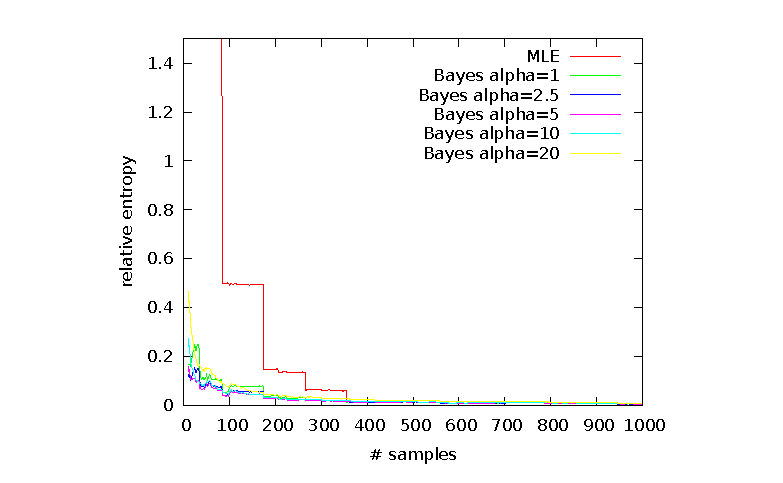
\includegraphics[scale=0.95]{fig/kl-cancer}
        \caption{\uv{Cancer} network (5 variables, 10 parameters)}
    \end{subfigure}
    \quad
    \begin{subfigure}[b]{0.55\linewidth}
        \hspace{-2.8cm}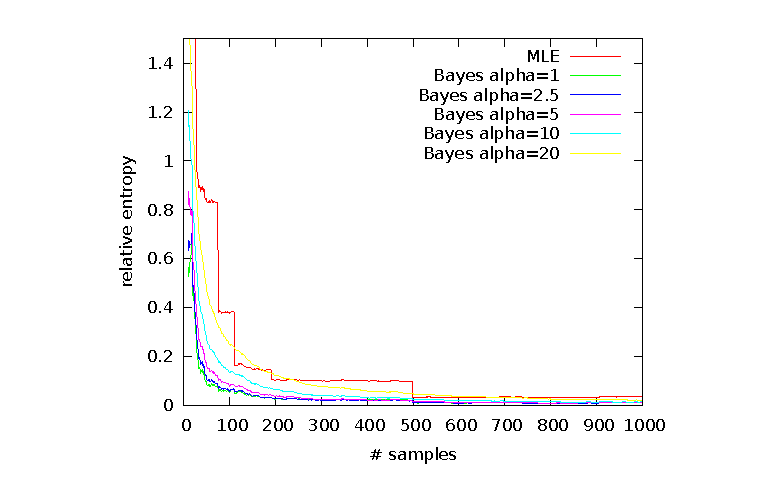
\includegraphics[scale=0.95]{fig/kl-asia}
        \caption{\uv{Asia} network (8 variables, 18 parameters)}
    \end{subfigure}
  
    \vspace{0.7cm}
    \begin{subfigure}[b]{0.55\linewidth}
        \hspace{-3.2cm}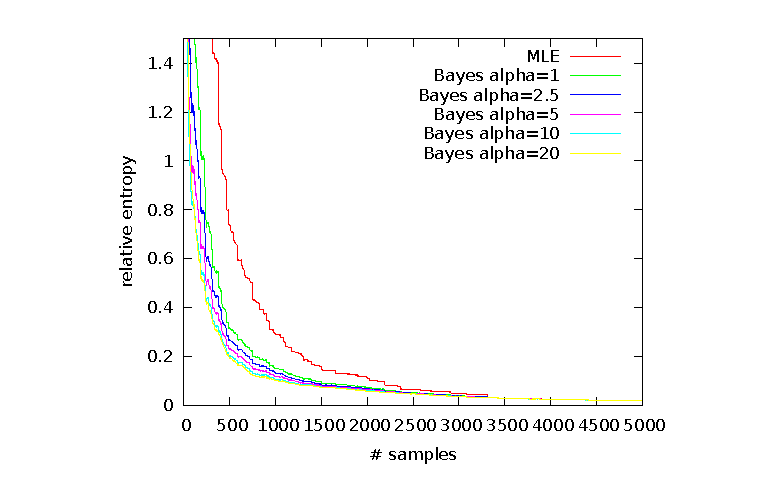
\includegraphics[scale=0.95]{fig/kl-child}
        \caption{\uv{Child} network (20 variables, 230 parameters)}
    \end{subfigure}
    \quad
    \begin{subfigure}[b]{0.55\linewidth}
        \hspace{-2.8cm}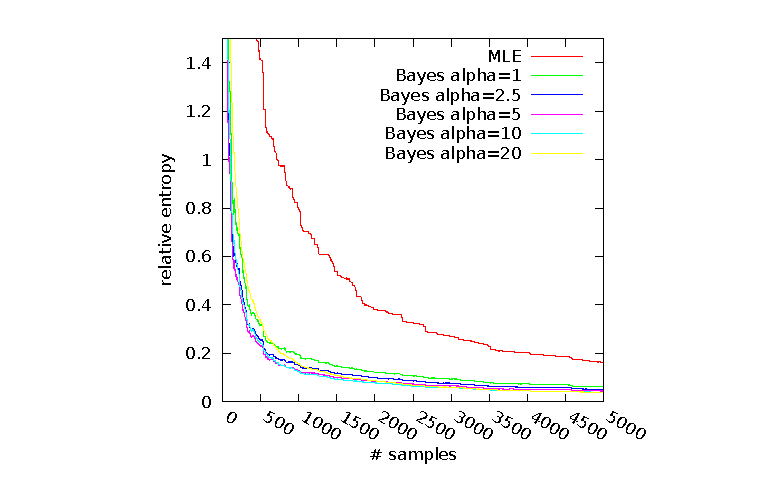
\includegraphics[scale=0.95]{fig/kl-icu}
        \caption{\uv{ICU alarm} network (37 variable, 509 parameters)}
    \end{subfigure}
    
    \caption{Performance analysis of parameter estimation methods for networks and datasets of various sizes using KL-divergence.}
    \label{fig:kl_div_benchmark}
\end{figure}

Also, according to the tests performed, MLE might seem to be steadily outperformed. Of course, if we had an excessive amount of training data, which is usually not the case in practice, then MLE would actually be more suitable than Bayesian estimation because the pseudosamples representing prior distribution for Bayesian estimation would turn into a hard-to-overcome source of inaccuracy.

If a concrete application demands estimated network parameters to be as close to the \uv{real ones} as possible, similar analysis, as I just performed, is a~sensible thing to do\,--\,pick a network of similar complexity, plot the learning curves for this network and determine what is the best parameter estimation method for dataset of given size.



\subsection{Learning structure}
Evaluation of structure learning proved to be a little problematic. We cannot directly use KL-divergence because the network structures aren't identical (although~\cite{heckerman95_learning} suggests a way of computing the KL-divergence) and other metrics for measuring distance of two probability distributions aren't suitable as they are based on exhaustive enumeration of atomic events and don't decompose over the network structure as KL-divergence does. Instead, I rely on manual inspection of the best-scoring network structures found over multiple runs of the learning algorithm. This approach is perfectly legal as I want to demonstrate usage of Bayesian networks in the field of data-mining which is a largely human-assisted discipline.

Because of I-equivalence there usually are multiple network structures sharing the same highest score and being, in a sense, equal. So, as a result of structure learning we might get a whole set of I-equivalent networks which differ only by direction of some edges. For such edges there is no clear causality between variables they connect, at least none that could be derived mathematically based on the dataset at hand, however, an expert may be able to decide the causality quite easily. So, not only we cannot tell whether any of the I-equivalent structures is better in terms of causality or in terms of explaining the data at hand, the learning algorithm driven by maximizing a scoring function cannot tell either. As we don't know the \uv{true} network structure, we need to inspect all the best-scoring structures. To ease the manual evaluation of structure learning I also maintain statistics for each pair of variables $U, V$ how often the final learnt structure contains the edge $U \rightarrow V$. This statistics is presented by a table in GUI.

As it turned out during my experiments, in context of Bayesian score the property whether or not two I-equivalent structures have the same score depends on the parameter prior we use. The simple K2 prior doesn't satisfy this property, the BDe prior does~\cite[p.~807]{pgm}. It is unfortunate because the K2 prior is easy to specify whereas a general BDe prior needs to be specified by creating a prior network (both network structure and its parameters). As a compromise I came up with a simple solution\,--\,I use BDe prior as if it were represented by a BN and as if the hyperparameters were inferred as $\alpha_{x \mid \vars{p}} = \alpha \cdot P'(x, \vars{p})$ where $P'$ is distribution induced by our prior BN. The trick is to make the prior BN discrete (without any edges) and to make prior distribution over each variable in the prior BN uniform. This way we get $\alpha_{x \mid \vars{p}} = \alpha / \bigl | val(\lbrace X \rbrace \cup Parents(X)) \bigr |$ quite elegantly without the need to perform any inference or to keep inner representation of the prior BN. Thereby the BDe prior is both easy to specify (only the value of $\alpha$ is needed) as well as it satisfies the property of I-equivalent structures having the same score.

\medskip
In my experiments I have found two I-equivalent structures to occur frequently. The first kind of structure a call a \term{chain}. A chain $X_1 - \dots - X_n$ is a structure in which variables $X_1, \dots, X_n$ are connected in a linear fashion in specified order $1,\dots,n$ with no V-structure and with no incoming edges to any of the variables; outcoming edges are unrestricted. At this point I introduce my own graphical notation for chains in Figure~\ref{fig:structure_learning_chain} (not to be confused with graphical notation of \term{plate models}~\cite{pgm}). Another set of I-equivalent structures, that also arises, I call \term{central variable structure}, meaning there is a \uv{central} variable $X$ and a set of variables $Y_1,\dots,Y_n$, all directly connected to $X$. At most one $Y$ variable may be parent of $X$ while all the other $Y$ variables are children of $X$. There are no other edges among the variables and also no incoming edges to the whole structure. All such central node structures are I-equivalent. Please see graphical notation of the central variable structure in Figure~\ref{fig:structure_learning_central_variable}.

\begin{figure}[ht]
    \centering
    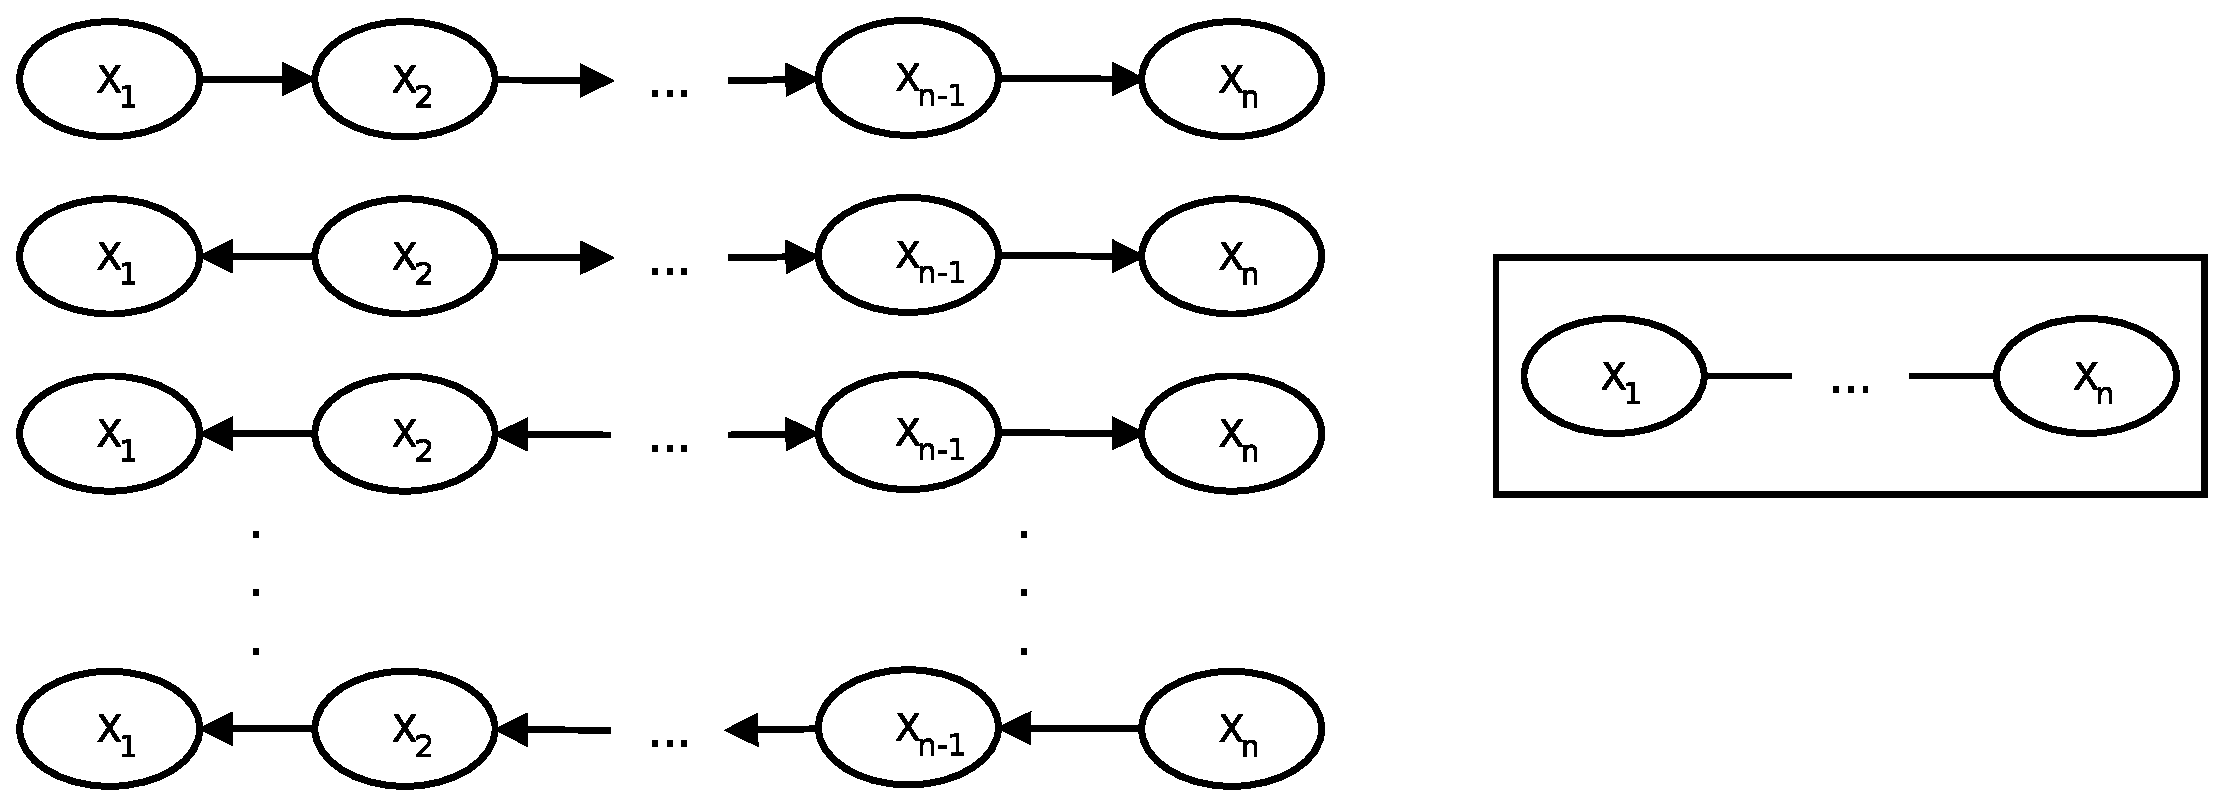
\includegraphics[scale=0.4]{fig/structure-learning-chain}
    \caption{A general chain $X_1 - X_2 - \dots - X_n$ of variables $X_1, \dots, X_n$ is a set of network structures where the variables are connected in a linear fashion in the order $1, \dots, n$ and there is no V-structure. Left side of this figure demonstrates the whole set of $n$ structures for the same chain and on the right side of this figure you see my own graphical notation for the whole set of chains (linear structure without edge directions enclosed in a box).}
    \label{fig:structure_learning_chain}
\end{figure}
\begin{figure}[ht]
    \centering
    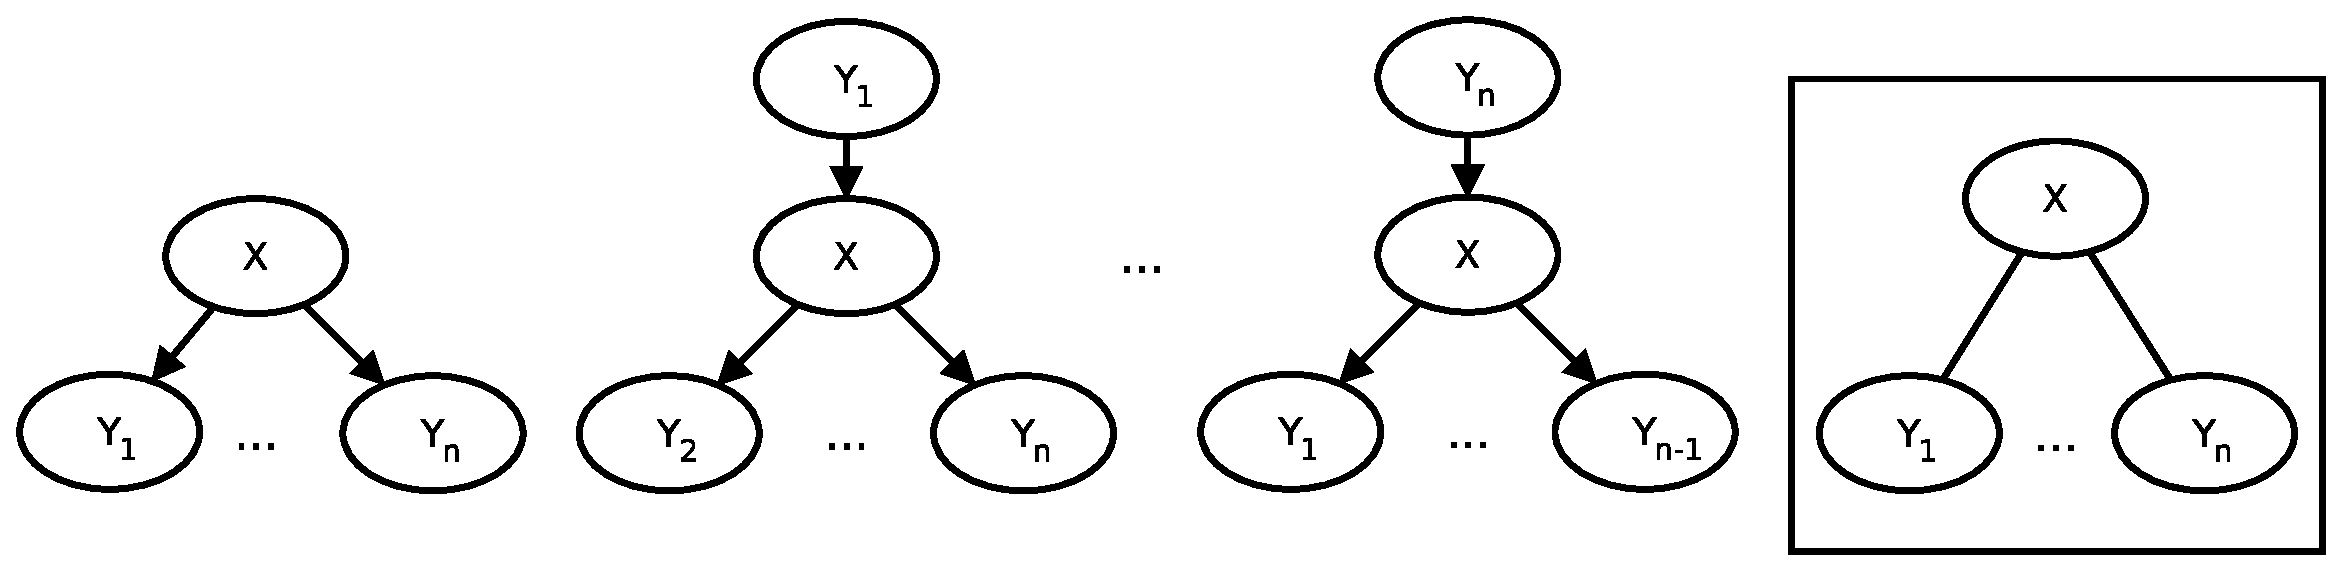
\includegraphics[scale=0.4]{fig/structure-learning-central-variable}
    \caption{Central variable structure $X,Y_1,\dots,Y_n$ is a set of I-equivalent structures where the $X$ variable is central in the sense that is connected with all $Y_i$ variables, at most one $Y_i$ variable is parent of $X$ and all the other $Y_i$ variables are children of $X$. There also may not be an incoming edge to any of the variables $X$ or $Y_i$ as that would potentially introduce a V-structure in some of the networks.
Structures without a bounding box represent the whole set of $n+1$ central variable structures and on the right side of this figure you can see my own graphical notation for the whole set of central variable structures.}
    \label{fig:structure_learning_central_variable}
\end{figure}

Results of the following experiments have been obtained primarily using the BIC score. The Bayesian score leads often to the same best-scoring structures and differences will be pointed out explicitly. \todo{The datasets I have used are available on the enclosed CD}.

Before we proceed to the experiments with structure learning please note that outcome of the experiments relies on the concrete dataset we sample before learning. So, for two datasets of equal size we quite frequently obtain different sets of best-scoring structures, especially when the number of samples is small (hundreds or thousands of samples, depending on the network).



\subsubsection{Experiments with the Cancer network}
The Cancer network with five variables is the simplest network I consider in my experiments. With a dataset of 300 samples the structure learning with BIC score discovers only a~chain $Xray - Cancer - Dyspnoea$, respectively its three I-equivalent variants, the variables $Smoker$ and $Pollution$ are isolated (see Figure~\ref{fig:structure-learning-cancer-300}).

With a dataset of 1\,000 samples the structure learning algorithm discovers only dependency among four variables in form of a central variable structure (see Figure~\ref{fig:structure-learning-cancer-1000}). The choice of central variable to be the $Cancer$ variable is consistent with the original network. The variable $Smoker$ is isolated in the found structures as $P(Cancer \mid Smoker)$ differs only by the value $0.02$ at maximum for different assignments of $Smoker$ and the potential edge $Smoker \rightarrow Cancer$ is in the score more penalized by the increase of structure complexity than it is favored for its contribution to the sum of family scores.

For a dataset with 5\,000 samples and the BIC score we finally obtain a connected graph, only there is similar situation as we had with 1000 samples\,--\,we obtain a central variable structure with $Cancer$ being the central variable (see Figure~\ref{fig:structure-learning-cancer-5000}). The results of this and of the previous test suggest that V-structures need to be strongly implied by the dataset, otherwise the learning algorithm will avoid introducing a V-structure.

Finally, with a dataset of 20\,000 samples the learning process with the BIC score yields the exact original structure of cancer network and no others (see Figure~\ref{fig:structure-learning-cancer-20000}). The original structure is unique as it contains a V-structure in $Cancer$ variable which spoils any possibility for there being a chain of variables that could be somehow rearranged. With the Bayesian score and $\alpha=0.1$ we still obtain the central variable structure as in Figure~\ref{fig:structure-learning-cancer-5000} even with a~dataset this big. The exact original structure is found with a dataset of 30\,000 samples. With $\alpha \in [1, 10]$ the exact structure is found also with 20\,000 samples.

\begin{figure}[ht]
    \centering
    \begin{subfigure}[b]{0.45\linewidth}
        \centering
        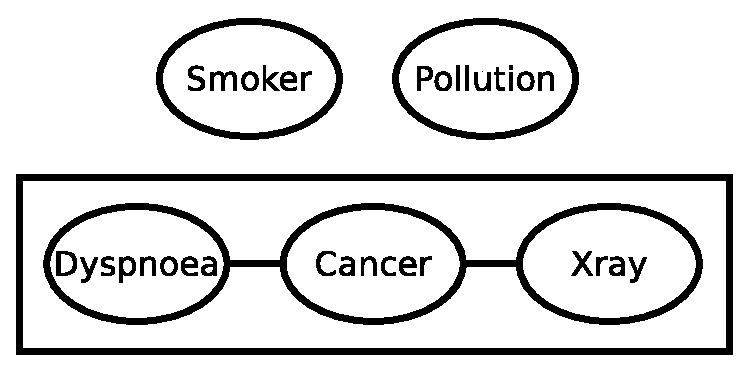
\includegraphics[scale=0.4]{fig/structure-learning-cancer-300}
        \caption{Dataset of 300 samples, 3 I-equivalent structures.}
        \label{fig:structure-learning-cancer-300}
    \end{subfigure}
    \quad
    \begin{subfigure}[b]{0.45\linewidth}
        \centering
        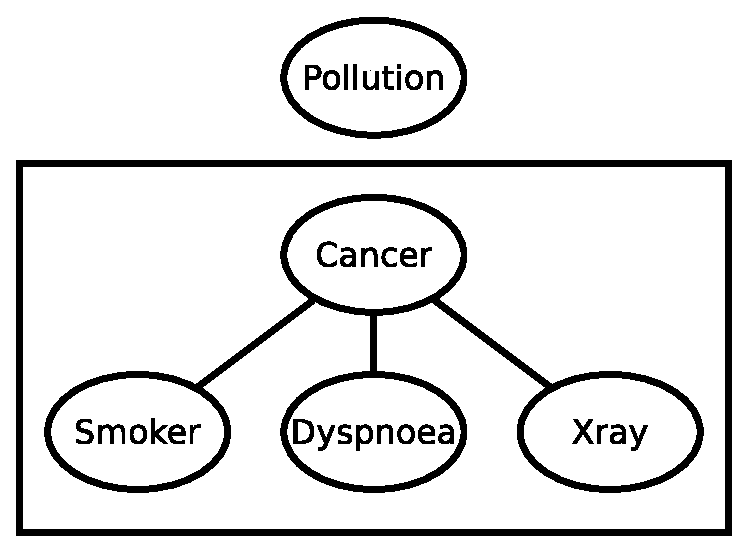
\includegraphics[scale=0.4]{fig/structure-learning-cancer-1000}
        \caption{Dataset of 1\,000 samples, 4 I-equivalent structures.}
        \label{fig:structure-learning-cancer-1000}
    \end{subfigure}
        
    \begin{subfigure}[b]{0.45\linewidth}
        \centering
        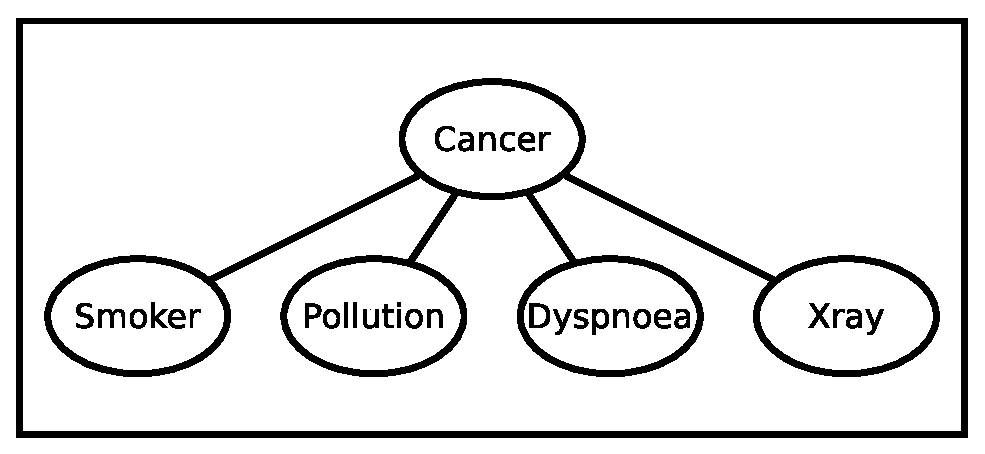
\includegraphics[scale=0.4]{fig/structure-learning-cancer-5000}
        \caption{Dataset of 5\,000 samples, 5 I-equivalent structures.}
        \label{fig:structure-learning-cancer-5000}
    \end{subfigure}
    \quad
    \begin{subfigure}[b]{0.45\linewidth}
        \centering
        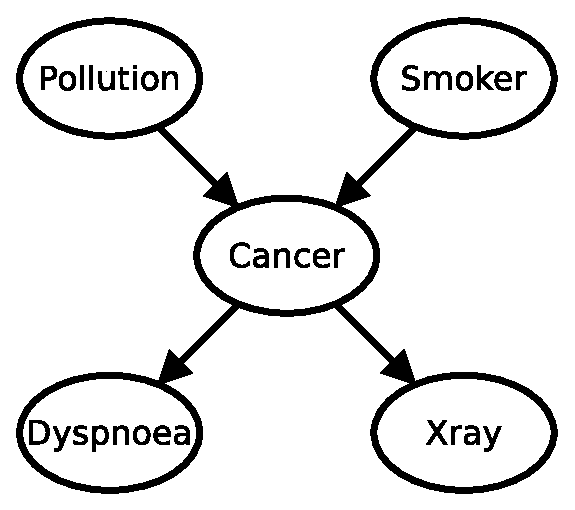
\includegraphics[scale=0.4]{fig/structure-learning-cancer-20000}
        \caption{Dataset of 20\,000 samples, single structure (exactly the original Cancer network).}
        \label{fig:structure-learning-cancer-20000}
    \end{subfigure}
    \caption{Best-scoring I-equivalent network structures found for the Cancer network with datasets of various sizes using the BIC score.}
    \label{fig:structure-learning-cancer}
\end{figure}

Parameters of the experiments: 200 runs, 200 iterations per run, 15 random restart steps, 0.15 relative size of tabu-list, maximum of 3 parents, $\alpha \in [0.1, 10]$.


\subsubsection{Experiments with the Asia network}
The Asia network contains 8 variables and a single V-structure $Either \rightarrow Dysp \leftarrow Bronc$. The CPD for $Dysp$ variable suggest strong dependency on both its parents\,--\,the distribution $P(Dysp \mid Either, Bronc)$ changes by up to $0.7$ for different assignments of $Either$ and by up to $0.6$ for different assignments of $Bronc$. Therefore for as little as 100 samples the found networks contain the V-structure at the $Dysp$ variable. Furthermore, $Dysp$ has always the same set of parent variables but that can be accounted to the strong dependency in the original network.

With a dataset of 1\,000 samples we almost get structures I-equivalent to the original network (see Figure~\ref{fig:structure-learning-asia-1000}), only the variable $Asia$ is isolated thanks to a weak dependency $Asia - Tub$. There are three I-equivalent structures because variables $Smoke - Bronc - Lung$ form a chain, structure of the other variables is the same as in the original network. 

For a dataset of 15\,000 samples we obtain the complete structure of the Asia network, respectively six I-equivalent variants of the original network (see Figure~\ref{fig:structure-learning-asia-15000}) thanks to two chains $Lung - Smoke - Bronc$ and $Asia - Tub$ which are present in the original network.

In the case of the Asia network the Bayesian score worked best with $\alpha=1$. With higher values of $\alpha$ (eg. 5 or 10) the learnt networks contained additional edges and V-structures that aren't present in the original network.

\begin{figure}[ht]
    \centering
    \begin{subfigure}[b]{0.45\linewidth}
        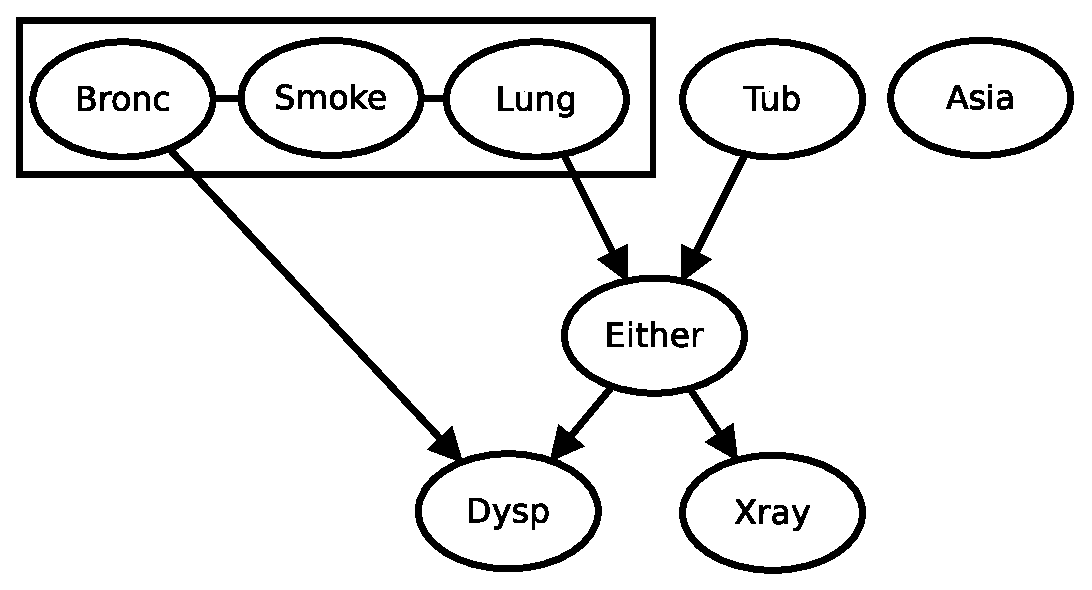
\includegraphics[scale=0.4]{fig/structure-learning-asia-1000}
        \caption{Dataset of 1000 samples, 3 I-equivalent structures.}
        \label{fig:structure-learning-asia-1000}
    \end{subfigure}
    \qquad
    \begin{subfigure}[b]{0.45\linewidth}
        \centering
        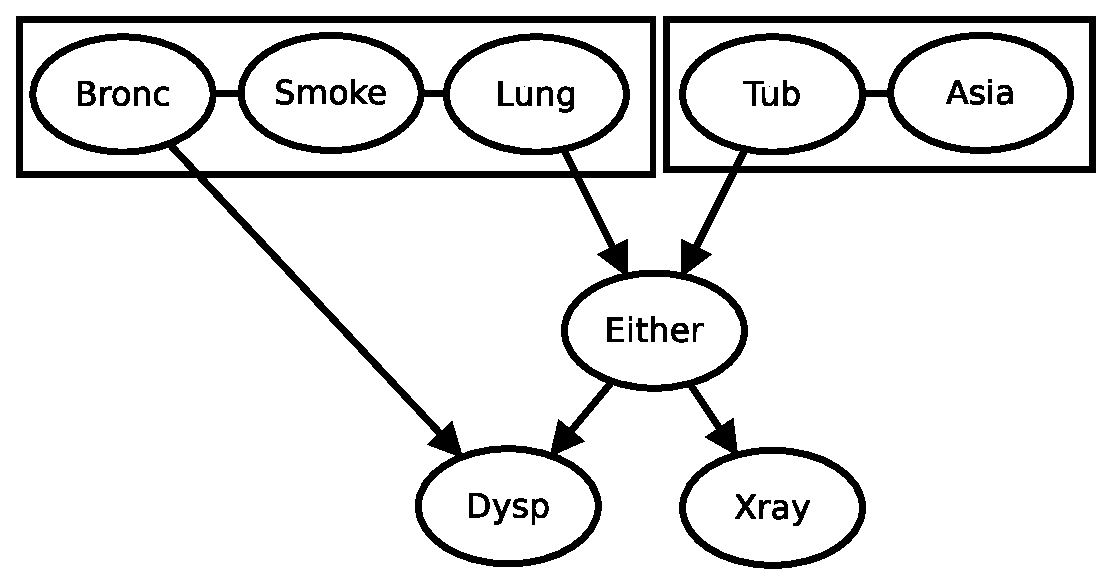
\includegraphics[scale=0.4]{fig/structure-learning-asia-15000}
        \caption{Dataset of 15000 samples, 6 structures I-equivalent with the original network.}
        \label{fig:structure-learning-asia-15000}
    \end{subfigure}
    \caption{Best-scoring I-equivalent network structures found for the Asia network with datasets of various sizes (same results for the BIC score and the Bayesian score).}
    \label{fig:structure-learning-asia}
\end{figure}

Parameters of the experiments: 200 runs, 200 iterations per run, 15 random restart steps, 0.15 relative size of tabu-list, maximum of 3 parents, $\alpha=1$.



\subsubsection{Experiments with the Child network}
The Child network is a bit larger, contains 20 variables, 6 V-structures and one variable with high number of children (the $Disease$ variable with 7 children). At first we will inspect the best structures found with datasets of different sizes (best in the sense of minimal differences from the original network) and explore what inconsistencies they have. Then we will discuss how to proceed when attempting to find the best structure when the original structure is unknown.

With a dataset of 500 samples and the BIC score the structure learning yields a structure with two isolated variables ($Age$ and $BirthAsphyxia$), the rest of the network is to an almost surprisingly high degree consistent with the original network, considering how little samples we have (see Figure~\ref{fig:structure-learning-child-500-bic}). The best-scoring networks contain four V-structures out of the six which are present in the original network, again suggesting that once a V-structure is learnt, it is a fairly stable feature of the network unlike a chain or a central variable structure. When not considering edge directions, the learnt network is missing 4~out of 25 connections present in the original network and from the remaining 21 edges up to three may be reversed due to chain structures. There is one obvious chain structure $Disease - LVH - LVHreport$ causing three I-equivalent variants of the learnt network. Notice that when the edge $Disease - LungParench$ is reversed then $LungParench - CO2 - CO2Report$ effectively becomes another chain structure because then there are no incoming edges to any of these variables (edges that might be reversed are painted in gray). In either case, only those variants of the chain structures are allowed such that they don't introduce a V-structure in the $Disease$ variable as this would imply conditional dependencies and marginal independencies that aren't supported by the data. Furthermore, in the learnt network there isn't any redundant connection that wouldn't be in the original network.

With the Bayesian score and 500 samples the best result is similar to that of the BIC score (achieved using $\alpha=2.5$, see Figure~\ref{fig:structure-learning-child-500-bayes-2_5}). The only difference is that the edge $Disease - DuctFlow$ is reversed instead of allowing for variations of the chain structure $Disease - LVH - LVHreport$. I believe this difference may be caused by a local maximum in the Bayesian scoring function which makes it for the optimization algorithm difficult to find the I-equivalent structures which the BIC score does find.

\begin{figure}[ht]
    \centering
    \begin{subfigure}[b]{0.45\linewidth}
        \hspace{-2.3cm}
        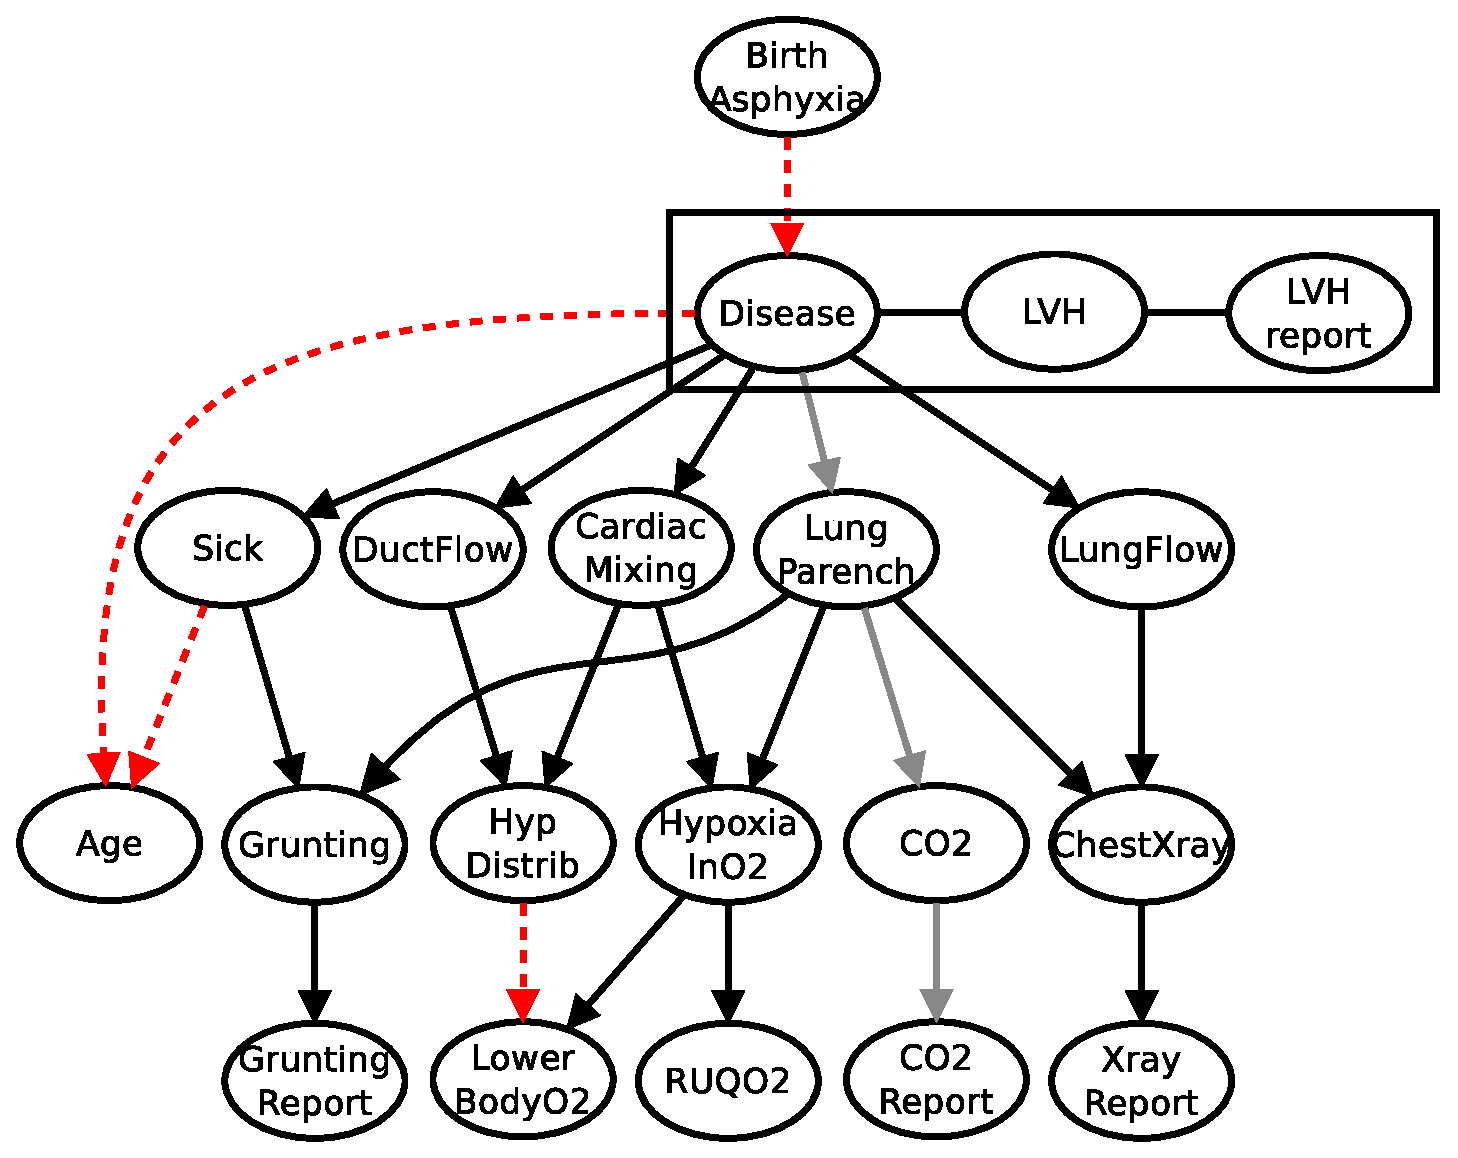
\includegraphics[scale=0.37]{fig/structure-learning-child-500-bic}
        \caption{Using the BIC score.}
        \label{fig:structure-learning-child-500-bic}
    \end{subfigure}
    \begin{subfigure}[b]{0.45\linewidth}
        \hspace{-0.5cm}
        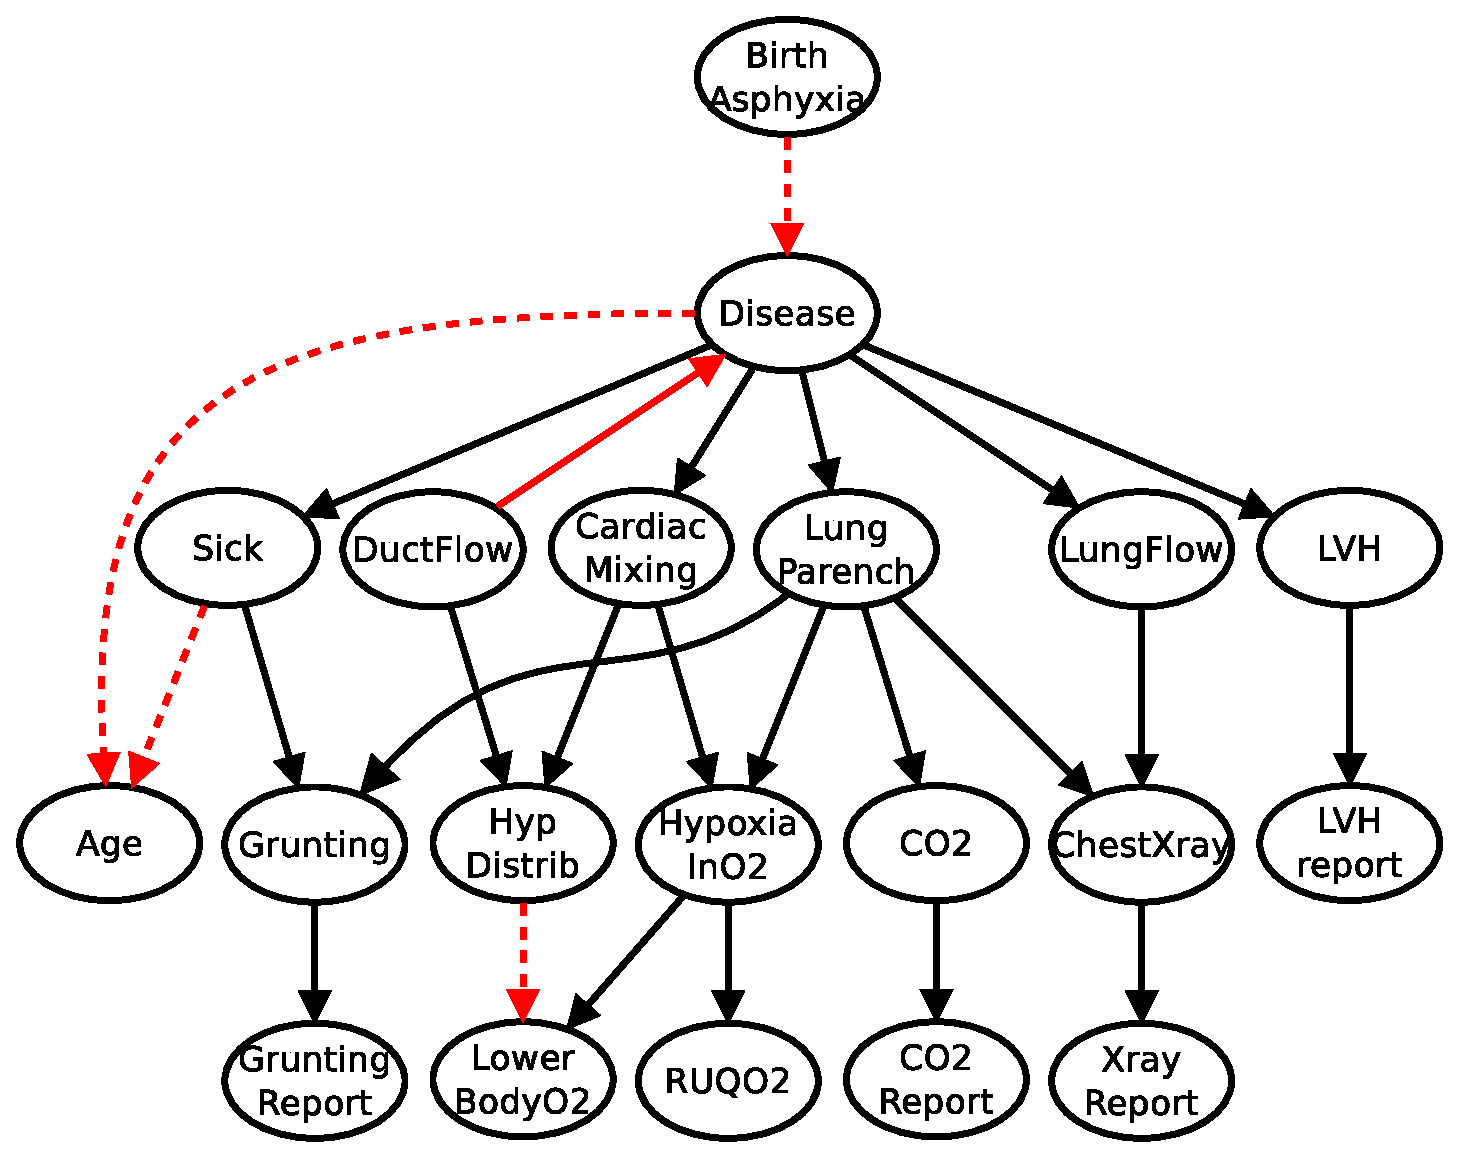
\includegraphics[scale=0.37]{fig/structure-learning-child-500-bayes-2_5}
        \caption{Using the Bayesian score with $\alpha = 2.5$.}
        \label{fig:structure-learning-child-500-bayes-2_5}
    \end{subfigure}
    \caption{Best-scoring network structure found for the Child network with a dataset of 500 samples.
    \\Legend: Red dotted edges are missing, red edges are reversed, gray edges may be reversed (under conditions stated in the text).}
\end{figure}

With a dataset of 2\,000 samples and the BIC score we get a connected graph in which only the edge $Sick - Age$ is missing and one or two of many edges may be reversed (see Figure~\ref{fig:structure-learning-child-2000-bic}). There are many chain structures involving the $Disease$ variable (one with three variables, expressed by the boxed graphical notation, and seven chain structures with two variables, expressed with a gray edge instead). Legal variants of the chain structures are only those that don't introduce a V-structure in the $Disease$ variable, eg. if $Age$ were parent of $Disease$ then no other variable of the other chain structures may be a~parent of $Disease$. Furthermore, if the edge $Disease - LungParench$ is reversed then $LungParench - CO2 - CO2Report$ effectively become a chain because then there is no incoming edge to any of those variables.

With the Bayesian score (best results achieved with $\alpha=2.5$, see Figure~\ref{fig:structure-learning-child-2000-bayes-2_5}) and 2\,000 samples the learnt structure has no isolated variable, it is missing the edge $Sick - Age$, just as with the BIC score, and only two edges are reversed which is a particularly nice result.

\begin{figure}[ht]
    \centering
    \begin{subfigure}[b]{0.45\linewidth}
        \hspace{-2.5cm}
        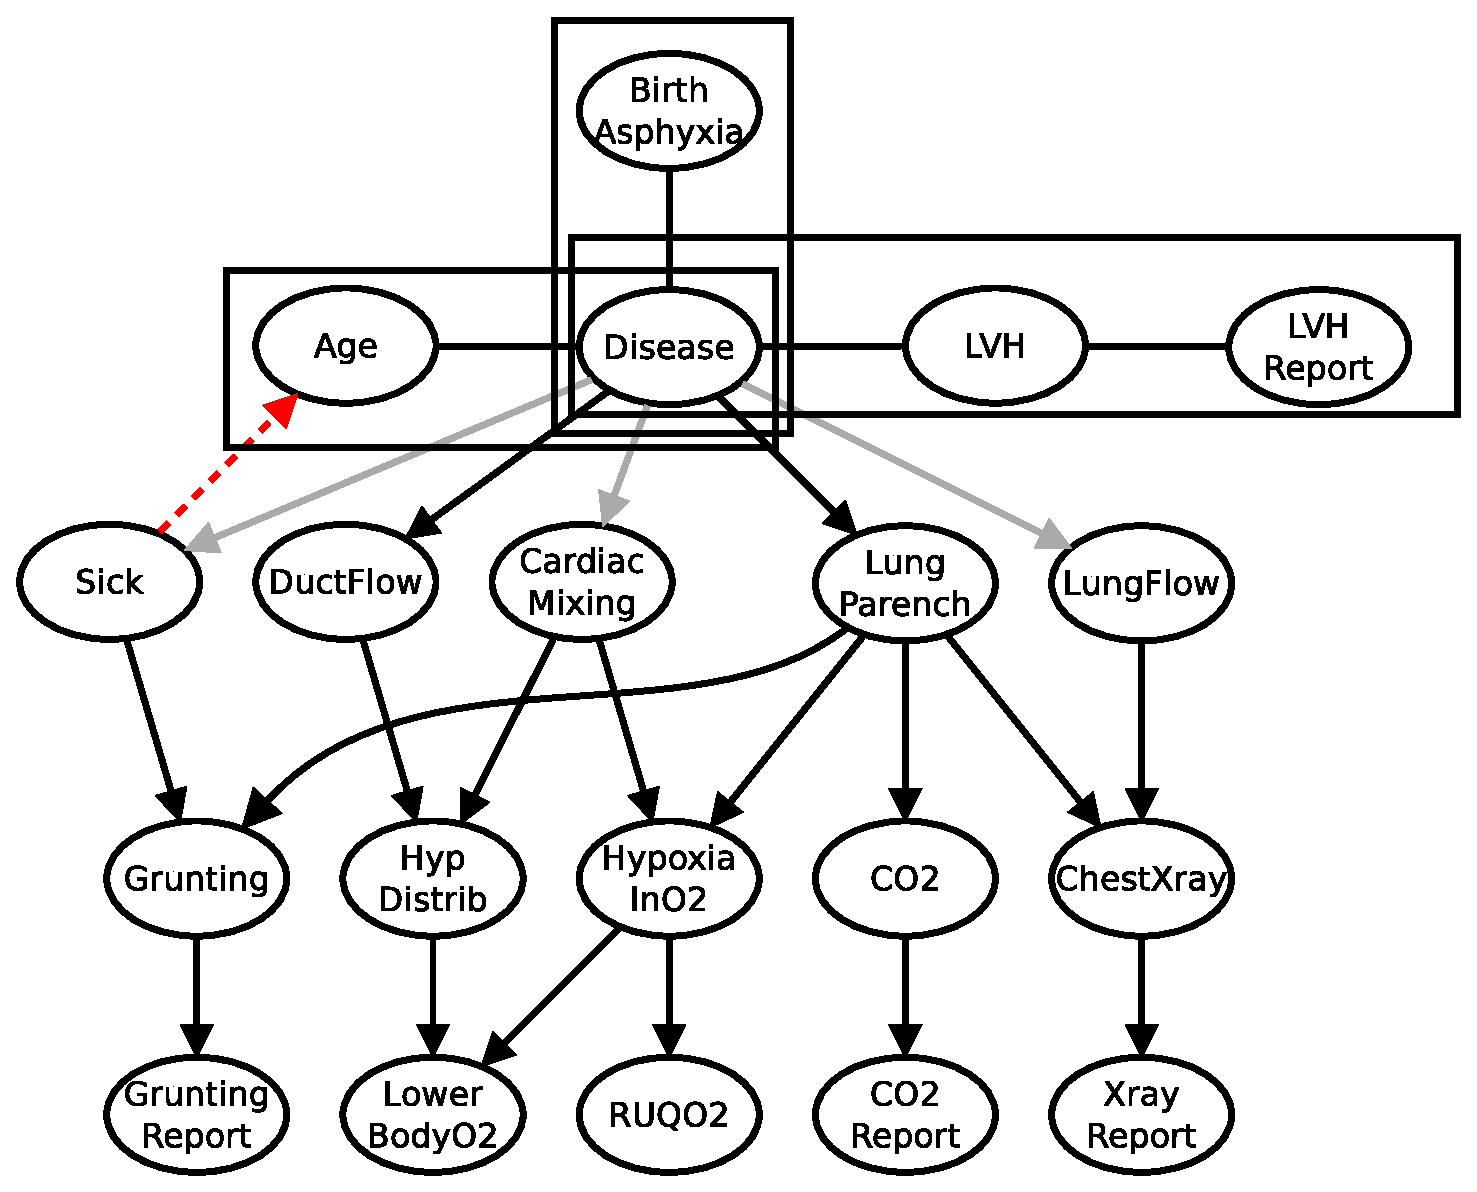
\includegraphics[scale=0.37]{fig/structure-learning-child-2000-bic}
        \caption{Using the BIC score.}
        \label{fig:structure-learning-child-2000-bic}
    \end{subfigure}
    \begin{subfigure}[b]{0.45\linewidth}
        \hspace{-0.7cm}
        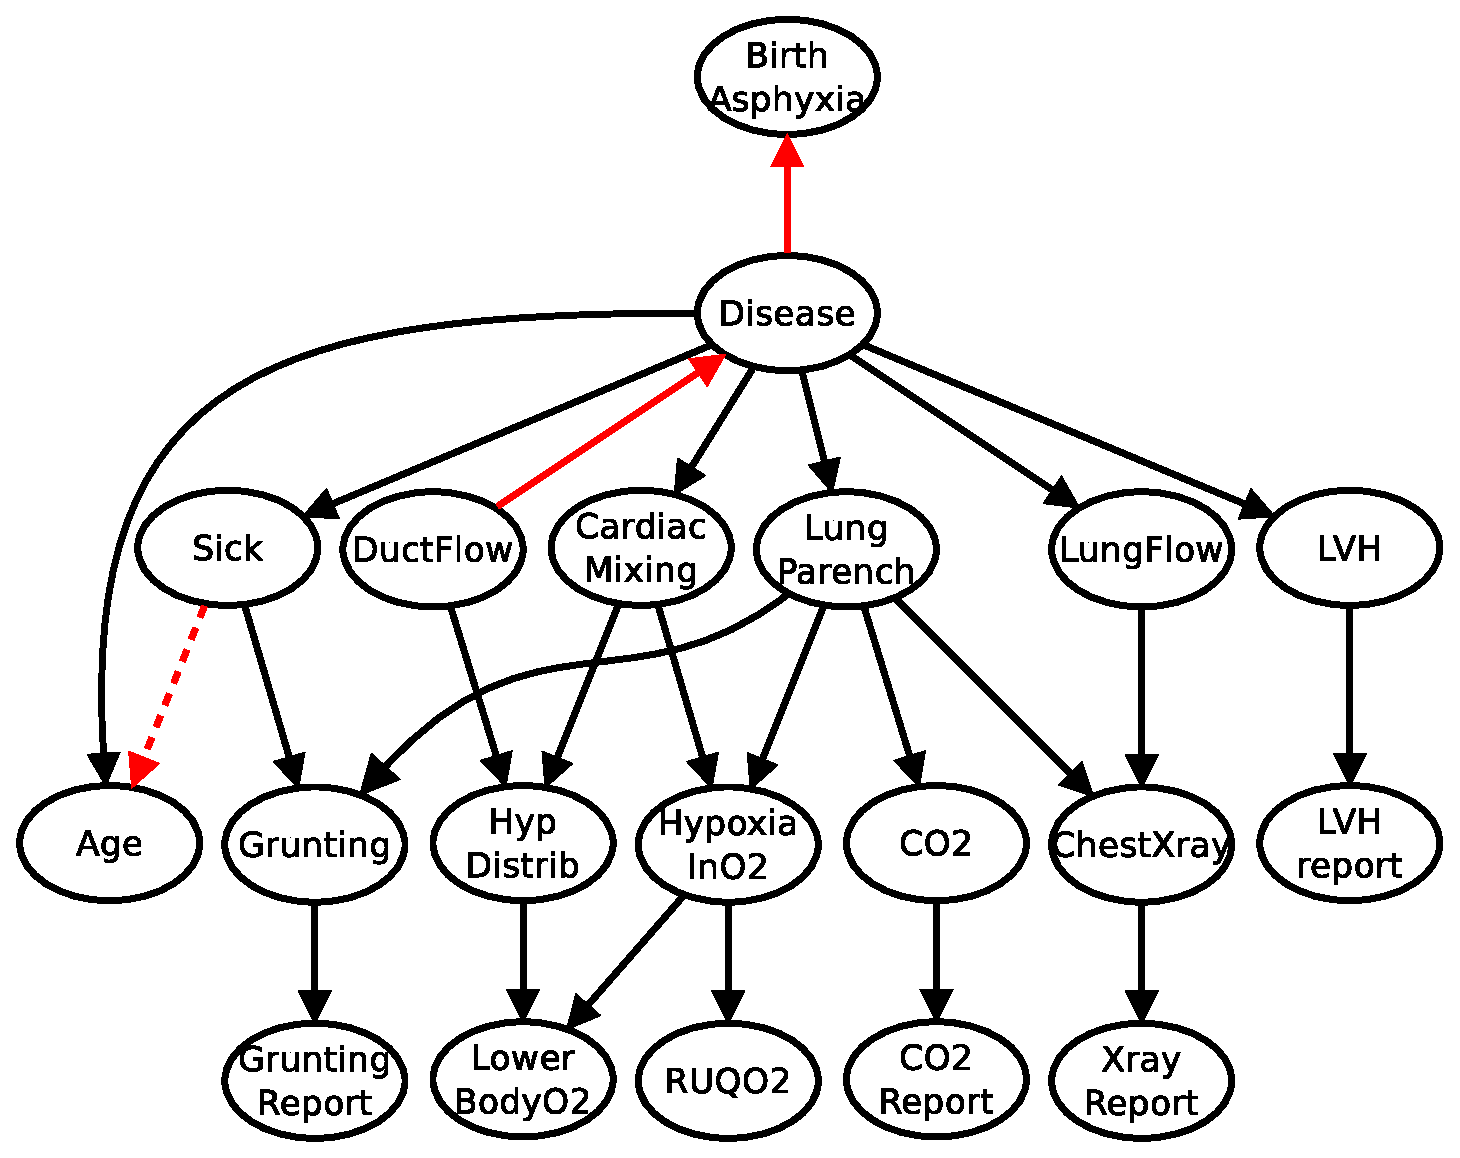
\includegraphics[scale=0.37]{fig/structure-learning-child-2000-bayes-2_5}
        \caption{Using the Bayesian score with $\alpha = 2.5$.}
        \label{fig:structure-learning-child-2000-bayes-2_5}
    \end{subfigure}
    \caption{Best-scoring network structure found for the Child network with a dataset of 2\,000 samples.
    \\Legend: Red dotted edges are missing, red edges are reversed. One of the gray edges may be reversed if it doesn't introduce a V-structure in the $Disease$ variable wrt. concrete variants of the other chain structures in the $Disease$ variable.}
\end{figure}

Dataset of 5\,000 samples and the BIC score get us as close to the original network as no missing connections, three reversed edges and one redundant edge. The mistake introduced by the redundant edge is somewhat local, involving a closed structure of three nodes $LungParench$, $CO2$ and $CO2Report$ (see Figure~\ref{fig:structure-learning-child-5000-bic}) and no other variables are involved. Curious thing is that there has actually been formed a V-structure in the $CO2$ variable which might be caused by noise in the used dataset.

The Bayesian score (best with $\alpha=3$, see Figure~\ref{fig:structure-learning-child-5000-bayes-3_0}) in this particular test did significantly better than the BIC did. They both agree on the reversed edge $Disease - BithAsphyxia$ and, other than that, with the Bayesian score there is only one reversed edge and no redundant edges.

\begin{figure}[ht]
    \centering
    \begin{subfigure}[b]{0.45\linewidth}
        \hspace{-2.3cm}
        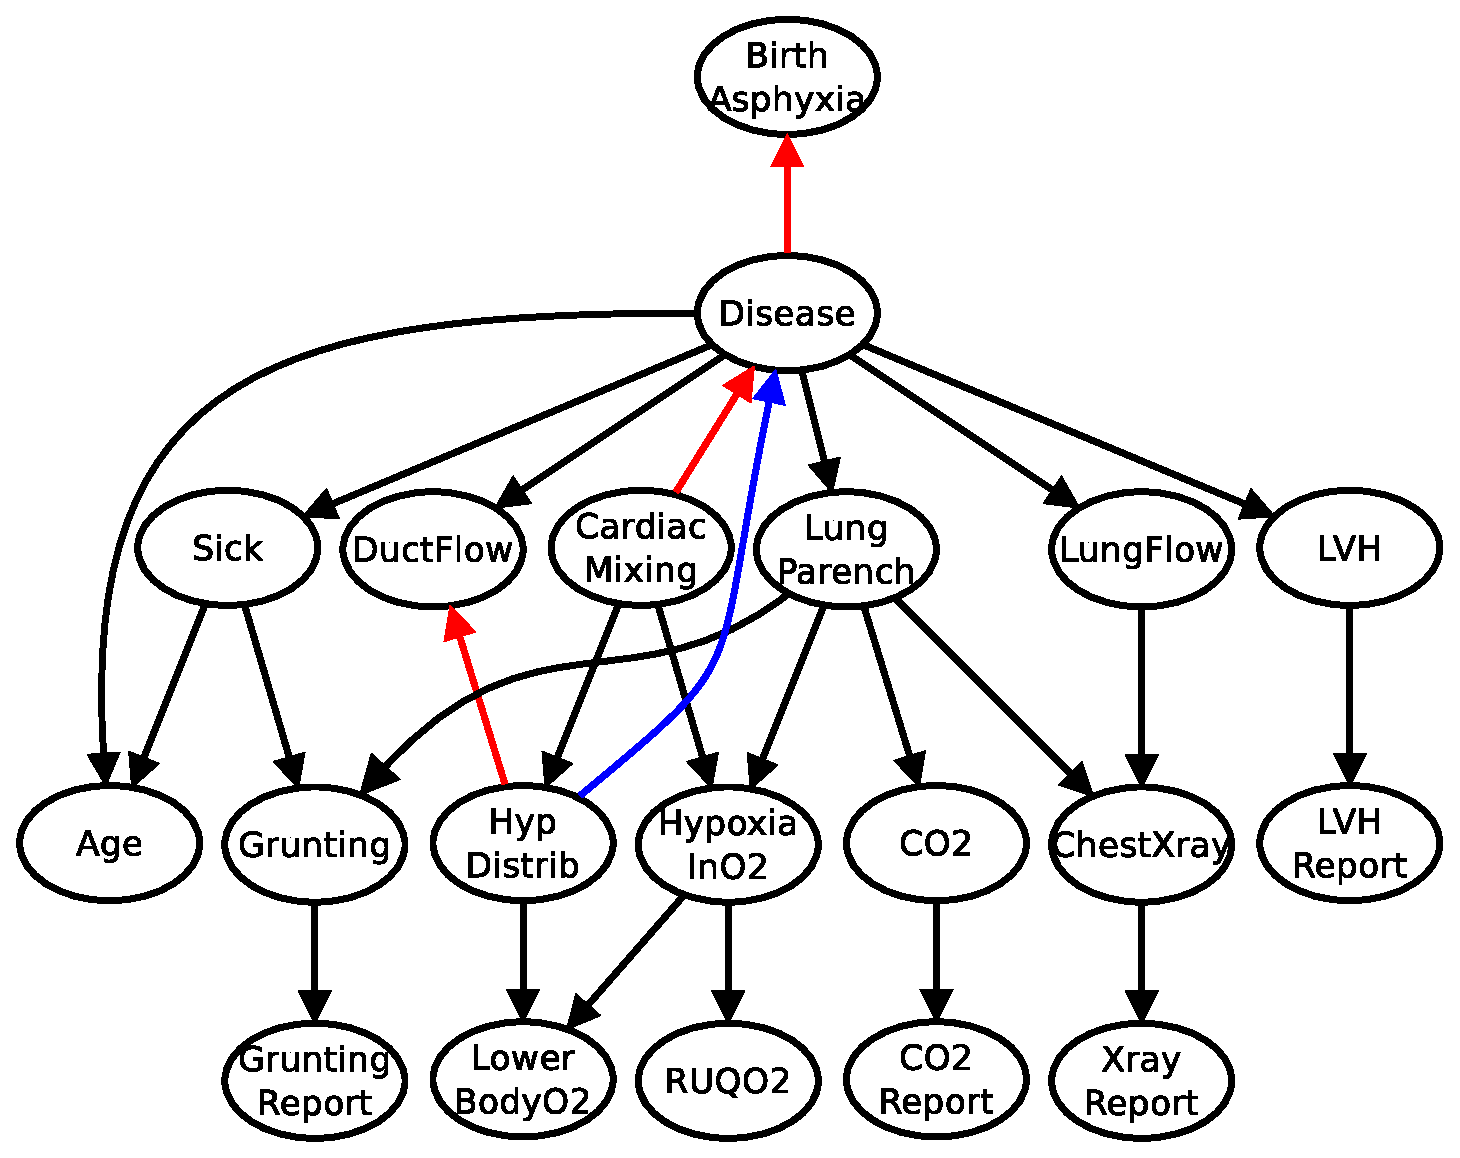
\includegraphics[scale=0.37]{fig/structure-learning-child-5000-bic}
        \caption{Using the BIC score.}
        \label{fig:structure-learning-child-5000-bic}
    \end{subfigure}
    \begin{subfigure}[b]{0.45\linewidth}
        \hspace{-0.1cm}
        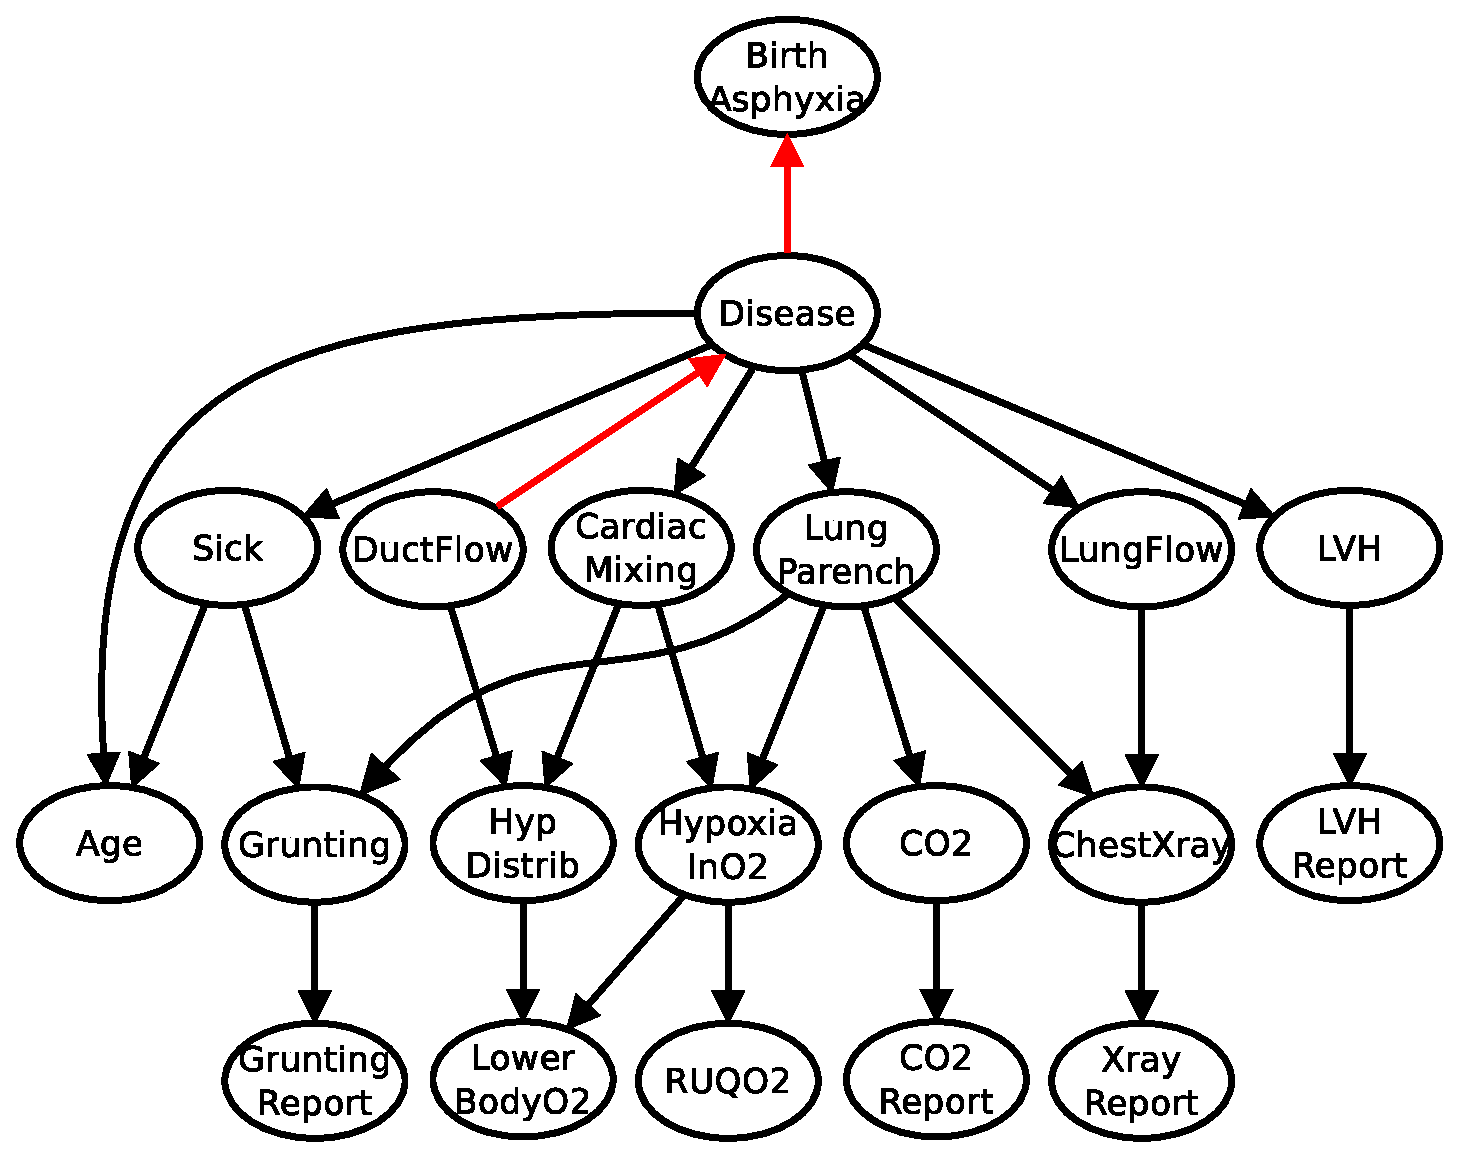
\includegraphics[scale=0.37]{fig/structure-learning-child-5000-bayes-3_0}
        \caption{Using the Bayesian score with $\alpha = 3$.}
        \label{fig:structure-learning-child-5000-bayes-3_0}
    \end{subfigure}
    \caption{Best-scoring network structure found for the Child network with a dataset of 5\,000 samples.
    \\Legend: Red dotted edges are missing, red edges are reversed, blue edges are redundant.}
\end{figure}

\medskip
In a situation when our goal is to discover the original structure the question is how to pick the right equivalent sample size $\alpha$ for the Bayesian score so that the learnt structure would be as close as possible to the correct one. For a range of $\alpha$ values I have inspected the relation between Bayesian score of a learnt structure and how closely the learnt structure matches the original one. I have found out that within the approximate range $\alpha \in [1,4]$ structure with the highest score is also the closest. 
I have made the observation that higher value of $\alpha$ means higher chance of the learnt network having an extra edge and also doesn't improve the number of reversed edges. So, $\alpha$ should be kept at a small value.
It is true that with higher values of $\alpha$ we can discover a structure with even better Bayesian score but, in my experience, this structure typically has some redundant edges that aren't present in the original network and also the number of other deviations isn't pleasing. So, when attempting to learn the best possible structure (and the number of variables is comparable with the child network) we should try the learning procedure for $\alpha \in [1,4]$ with a step $0.5$ and pick the $\alpha$ such that the Bayesian score of the learnt structures is the highest.

\begin{comment}
\begin{figure}[p]
    \vspace{-1cm}
    \centering
    \begin{subfigure}[b]{1\linewidth}
        \centering
        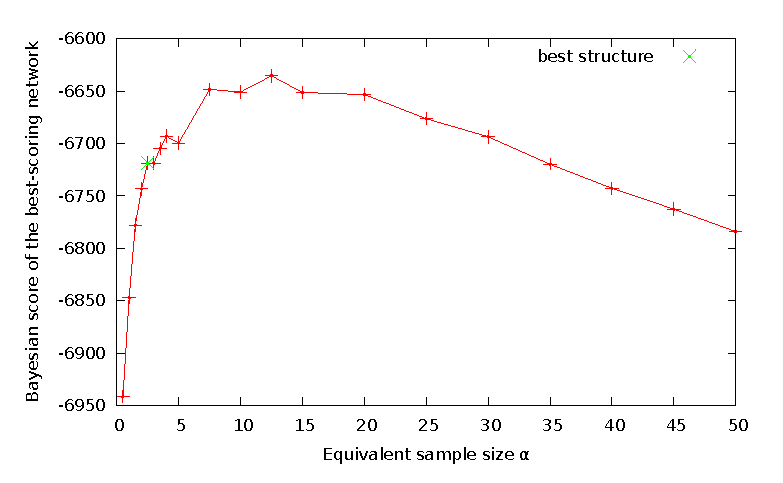
\includegraphics[scale=0.85]{fig/child-500-alpha-score}
        \caption{500 samples}
    \end{subfigure}
    \\ \vspace{0.3cm}
    \begin{subfigure}[b]{1\linewidth}
        \centering
        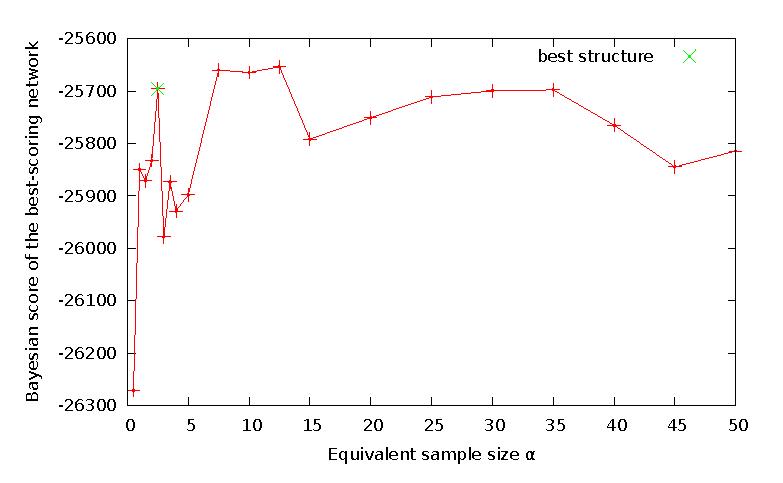
\includegraphics[scale=0.85]{fig/child-2000-alpha-score}
        \caption{2\,000 samples}
    \end{subfigure}
    \\ \vspace{0.3cm}
    \begin{subfigure}[b]{1\linewidth}
        \centering
        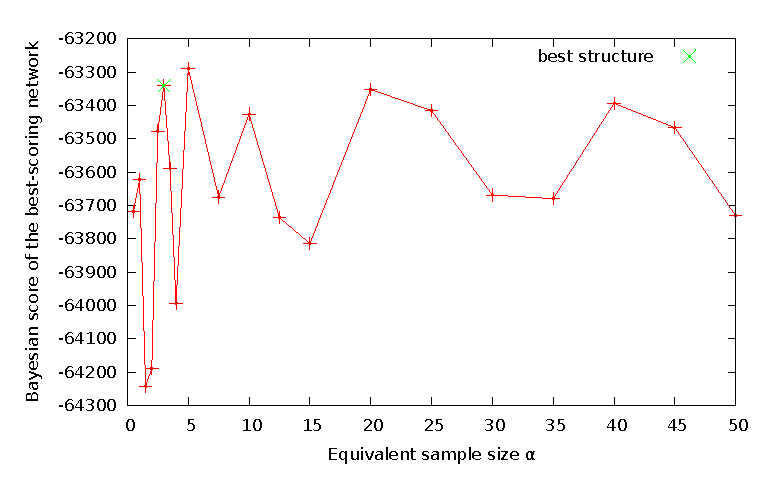
\includegraphics[scale=0.85]{fig/child-5000-alpha-score}
        \caption{5\,000 samples}
    \end{subfigure}
    \caption{Bayesian scores of the best-scoring structures for different values of $\alpha$ and datasets of various sizes. The structure, that resembles the original network the most, is always found with $\alpha$ within the approximate range $[1,4]$.}
    \label{fig:structure-learning-child-alpha-analysis}
\end{figure}
\end{comment}


\medskip
Parameters of the learning procedure: 1\,000 runs, 600 iterations per run, 50 random restart steps, 0.15 relative size of tabu-list, maximum of 4 parents, $\alpha \in [1.5, 3]$.




\subsubsection{Conclusion of the the experiments}
Based on the experiments regarding structure we can make some general observations:
\begin{itemize}
    \item There are often more than one best-scoring structures due to I-equivalence and, with some practice, chain structures and central variable structures are actually relatively easy to spot. Other than these two types of structures we sometimes observe swapping two variables $B,C$ in a cascade of the form $A-B-C$ while preserving edge $A \rightarrow B$ and introducing an edge $A \rightarrow C$. The experiments suggest that such mistakes are just local and don't involve other variables.
    \item V-structures introduce conditional dependencies and marginal independencies, therefore a V-structure is not learnt unless it is strongly implied by the data and incorrect V-structures are rare (for reasonable values of $\alpha$ of Bayesian score).
    \item Best value of $\alpha$ for the Bayesian score is usually relatively small\,--\,for the used networks and datasets the best values of $\alpha$ were from the interval $[1,3]$ in all cases. Also, for $\alpha \in [1,3]$ learnt structures with higher Bayesian score were generally closer to the original network. This provides us with a powerful rule of thumb on how to determine the right $\alpha$ when learning a~network structure whose original structure is unknown to us\,--\,look for a local maximum in the scores of learnt networks for $\alpha$ within the range about $[1,4]$.
    \item The Bayesian score is more conservative, the BIC score often leads to a specific structure close to the original one faster (with a smaller dataset) whereas the Bayesian score requires a larger dataset. Although with a tuned value of $\alpha$, results with the Bayesian score may be the same or even better than those of the BIC score.
\end{itemize}



%\subsubsection{Optimal parameters for structure learning}
%I have performed a series of experiments to determine the optimal set of parameters for tabu-search algorithm (tabu-list size and random restart steps count) for networks of various degrees of complexity but, surprisingly, the space of achieved results turned out flat without any clear peaks suggesting a local maximum (metrics used were the average score of the resulting network and the relative frequency of finding the \uv{true} network, both taken from 1000 runs). Therefore I generally use random restart of about 25--50 steps and tabu-list size of 0.15-times the upper bound of feasible network alterations count. \todo{Try for the child network (best score found in 50 iterations or something like that.}





\section{Crime, its causes and countermeasures}\label{ch:practical_crime}
This application will take advantage of the fact that Bayesian networks are intuitive visual models that capture dependencies among random variables. With these ideas in mind BNs can be used to visualize the structure of a given domain in order to better understand the underlaying dynamics and relations within that domain.

In our particular problem we are given a dataset called \term{Communities and Crime}\footnote{The dataset \emph{Communities and crime} is available at \url{http://archive.ics.uci.edu/ml/datasets/Communities+and+Crime}.} containing records that describe various communities across the United States. A single record consists of features such as racial representation, income, family completeness attributes, housing etc. and the relative number of violent crimes in this community. Our goal is to find a BN that describes given data the best and that will hopefully provide us with some useful insight. Understanding dependencies among features can help us identify the main causes of crime, their relations and, based on these findings, to propose justified precautions.

\subsection{Data preprocessing}
Because the used dataset contains continuous features and because this thesis considers strictly discrete Bayesian networks we need to perform some kind of discretization. I~have applied binning to three equi-depth bins labeled $low$, $medium$ and $high$. Such discretization seems reasonable wrt. to the relatively small dataset and because the new values are, for a human, easily interpretable. Even with as little as three discrete values, four attributes $LemasPctOfficDrugUn$, $NumStreet$, $MedNumBR$, $pctUrban$\footnote{I use original names of attributes as they are in the Communities and crime dataset. Please see \srccode{.names} file on the enclosed CD for detailed description of all attributes.} are after the discretization uneven, ie. one of the bins is almost or entirely empty. So, we will keep in mind to primarily discard those attributes if some of them is member of a set of similar variables (will be explained later).

There is also a subset of attributes whose value is in roughly in 50\,\% of records unknown. Filling in such a big number of values, eg. based on some prediction model, doesn't seem reasonable. Therefore we discard those attributes altogether which leaves us with 100 attributes.


\subsection{Experiments}
%The main problem we face is that the preprocessed dataset contains 100 variables and if we attempt to learn a network with so many variables we won't be able to visually come up with any useful conclusion. That is why we will focus on reduction of the feature set to obtain interpretable networks.

I have tried to approach this data-mining task in several ways because the achieved results weren't as good as I had hoped. When using the complete dataset there were too many variables to see anything useful in the learnt network structure and when I attempted to somehow reduce the feature set, effect of many key variables on the target variable $ViolentCrimesPerPop$ (further referred to just as $Crime$) changed radically. Nevertheless, I believe that at least some useful information can be read from the models I have created.

To briefly elaborate, I have experimented with the following three approaches:
\begin{enumerate}
    \item[a)] Start with a collection of networks learnt using the Bayesian score with $\alpha_S \in [1, 15]$ and using the full feature set. Then, iteratively identify sets of variables that are in all the structures learnt with different $\alpha_S$ topologically close, have similar effect on the target variable (stimulating or suppressing) and their semantics is similar (eg. divorce rate of males vs. divorce rate of females or percentage of employed people vs. percentage of unemployed). Each such set of similar or antagonistic variables has been replaced by just one representative variable. This way I have managed to reduce the network from 100 variables to 67~variables within three iterations.
    
     To be more formal, variable $X$ and its representative $R$ influence the crime variable $C$ approximately the same way when $P(C \mid X) \approx P(C \mid R)$ or the opposite way when $P(C \mid X = low) \approx P(C \mid R = high)$, $P(C \mid X = medium) \approx P(C \mid R = medium)$ and $P(C \mid X = high) \approx P(C \mid R = low)$.
    These probability distributions are inferred by sampling after the network parameters are learnt using Bayesian estimation with $\alpha_P = 30$. The value of $\alpha_P$ has been chosen based on the KL-divergence analysis of parameter learning with the Hepar-II network\,--\,this network is the most similar I~could find to the learnt networks and also gives us a~good breathing space while the learnt networks get simpler through gradual elimination of attributes. In Figure~\ref{fig:kl_div_hepar2} we can see that for the Hepar-II network and 2\,000 samples, which is the size of our dataset, the value $\alpha_P = 30$ gets us closest to the original probability distribution.
    
    If it is the case that $P(C \mid X) \approx P(C \mid R)$ then mutual information of $X$ and $R$ has to be relatively high. To make the manual search of similar variables easier, mutual information of a pair of directly connected variables $X,R$ is visually represented in the program by color of the edge $X - R$ on \uv{cold-to-hot} color scale, ie. blue to red\footnote{In order to display mutual information between pairs of directly connected variables the current dataset has to be compatible with the current network and the option \srccode{Network -> Display edge weights} in the main menu needs to be checked.}.
    
    \item[b)] Start when the case~(a) ended. We cannot further apply the iterative elimination of similar attributes and 67 is still a large number of attributes. At this point, using the network structures learnt with the 67 attributes left, I analyzed what attributes influence the target variable $Crime$ the most, drop those attributes with least influence and finally, learn new network structures based on the surviving 52 attributes.
    
    To express the degree of influence some variable $X$ has on the target variable I~determine how significantly the target variable deviates from its prior distribution, which is the uniform distribution $(\frac{1}{3}, \frac{1}{3}, \frac{1}{3})$ due to binning, when $X$ is given, ie. for variable $X$ find the maximal value of $\Bigl\lvert 1/3 - P(Crime \mid X = x) \Bigr\rvert$ over all the networks learnt with various values of $\alpha_S$ and over all $x \in val(X)$. I will refer to this particular value as the \term{crime impact factor} of variable $X$. The probability distributions needed in order to determine the crime impact factor are, again, inferred by weighted sampling of a~network whose parameters have been learnt using the Bayesian estimation with $\alpha_P = 30$.
    
    \item[c)] Initially use the collection of networks learnt from the full feature set with various values of $\alpha_S$, as in the (a)~case. Then, right away analyze what attributes $X$ influence the target variable the most (using the crime impact factor introduced in~(b)), pick the top 40 most influential attributes and finally learn new network structures based on just the top 40 attributes.
\end{enumerate}

\begin{figure}[htb]
    \centering
    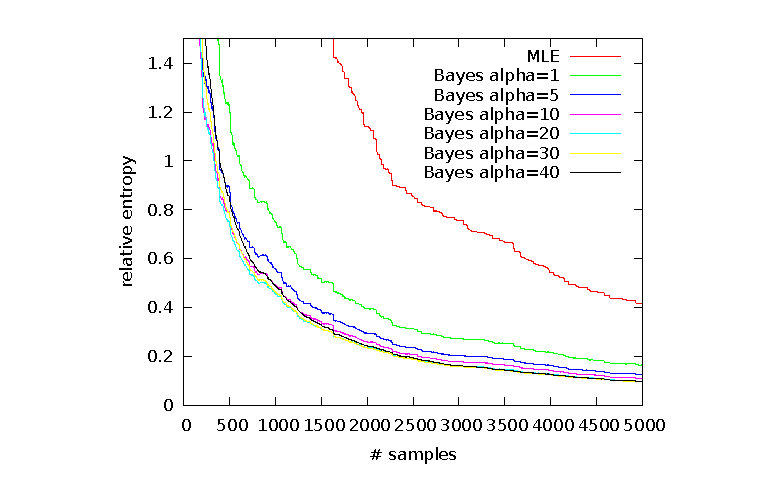
\includegraphics[scale=1.2]{fig/kl-hepar2}
    \caption{Performance analysis of parameter estimation methods for the Hepar-II network (70 variables, 1453 CPD entries). For a dataset of 2\,000 samples we can see that the Bayesian estimation with $\alpha=30$ is the best option.}
    \label{fig:kl_div_hepar2}
\end{figure}

Because we don't know the right parameter $\alpha_S$ of the Bayesian score for networks of this size and because the learnt networks differ in some edges, for each set of final networks we determine their structural intersection. In this context, by intersection I mean identifying those directed edges that are present in majority of the networks while tolerating a missing edge at most once (with 0 tolerance the networks contain too many isolated variables and with tolerance higher than one the networks become too dense). For the intersection network we compute crime impact factors of all variables, compare with crime impact factors in the original network and highlight variables that preserve the crime impact factor (green color) and those that have become totally misleading (red color). This way we can easily spot clusters of variables that are still relevant and ignore those that aren't. The structural intersection is computed from seven networks learnt using $\alpha_S \in \lbrace 1, 2, 5, 7.5, 10, 12.5, 15 \rbrace$.

\medskip
Now is the time to inspect the final networks for the cases (a), (b) and (c). In the first case we have in three iterations eliminated attributes that were, to some degree, duplicate and we have obtained the final network with 67~nodes shown in Figure~\ref{fig:crime_net_round3}. This network is still very big and in the printed version the variable names might not even be readable. This network is included only for the sake of completeness. Other than that it is hard, thanks to its structure, to read some useful information out of it. The target variable is significantly dependent only on the attributes capturing family completeness, illegal immigrants, racial representation and housing (variables whose crime impact factor is correct are highlighted in green, other than green are not considered because the results of analysis would be questionable). How exactly those variables affect the target variable $Crime$ can be easily determined by probabilistic queries which converge very fast. Generally, high divorce rate means high criminality. It can be seen that the illegal immigrants variable $PctIlleg$ and the $racepctblack$ variable are particularly negatively correlated with $PctFam2Par$. The key variable $PctPersDenseHous$ (suggesting ghettos or questionable city quarters) is positively influenced by the $PctIlleg$ variable and not so strongly influenced by the $racepctblack$ variable which is a little surprising. Still, based on the model we can conclude that illegal immigrants tend to live in big numbers within a small area which matches our general experience.

The (b)~case takes the variables that survived filtering in the (a)~case, determines crime impact factors of these variables and eliminates those with crime impact factor less than 0.07 which leads to a network with 53 nodes. Before we get into analyzing the network itself it is important to say that among other variables, that were eliminated because of low crime impact factor, was the $racePctAsian$ variable; also, this variable has low crime impact factor in the networks learnt using the full feature set. This fact suggests that the percentage of Asians is not very discriminative in terms of the target variable $Crime$, ie. that Asians in general don't significantly contribute to crime, not in the positive nor in the negative sense. Now we get to analyzing the learnt network shown in Figure~\ref{fig:crime_net_round4}. The variables, whose crime impact factors are correct, can be divided into two groups. The group of variables on the left from $Crime$ describes negative factors like illegal immigrants, dense housing, number of black people and people living on the street; most influential are $PctIlleg$, $racepctblack$ and $PctPersDenseHous$. There is also the variable reflecting the number of white people which is in very negative relation with all the other variables including $Crime$ (in other words, when speaking about crime, white people are generally well-behaved). The group of variables on the right from $Crime$ captures family completeness and wealth ($PctHousLess3BR$, $pctWWage$). The family completeness variables influence the $Crime$ variable heavily, the wealth variables aren't so powerful but there is still noticeable tendency of increased crime with lower wealth.

In the (c)~case we have analyzed crime impact factors of all variables right in the networks learnt using all 100 features and we have selected top 40 attributes with the highest crime impact factor to obtain the network shown in Figure~\ref{fig:crime_net_top40}. This network is probably the nicest of all we have learnt because it contains a single cluster of variables whose crime impact factor is correct and those variables are relatively densely connected, so we can expect that many of the real dependencies are actually reflected in the network. As opposed to the other two networks, in this network most of the family completeness variable, except for $PctKids2Par$, have incorrect crime impact factors. We can observe four smaller clusters of nodes describing mutually similar traits: (1)~the green cluster right above $Crime$ describing illegal immigrants, black and white people, people living on the streets or in shelters (this cluster has been present in the previous two networks as well); (2)~the green cluster forming a vertical belt on the left from $Crime$ capturing erudition, job quality and wealth; (3)~red cluster below $Crime$ with family completeness and wealth variables; (4)~red cluster on the far left with additional wealth and poverty variables. From cluster (1)~the most influential variables are in descending order $PctKids2Par$, $PctIlleg$, $racePctWhite$, $racepctblack$. The $NumInShelters$ variable is influenced mostly by the $NumIlleg$ variable meaning that illegal immigrants often seek refuge in shelters where they live at the expense of productive people and contribute to higher criminality. The variable $PctPersDenseHous$ is strongly influenced by illegal immigrants and, to lesser extent, also by $racepctblack$ which partly suggests the presence of ghettos. Variables from cluster (2)~aren't by far as powerful in terms of their effect on $Crime$ as variables of the first cluster but there is still a steady influence.


\medskip
Parameters of the learning procedure: 500 runs, 1\,500 iterations per run, 50 random restart steps, 0.1 relative size of tabu-list, maximum of 4 parents, $\alpha \in [1, 15]$.



\subsection{Conclusion}
This particular application of Bayesian networks turned out difficult and I found myself repeatedly in a dead end. Nevertheless, I believe that I have managed to find networks that correctly describe at least some aspects of the data. Maybe the most convincing argument is that in the learnt networks can be identified clusters of variables that capture similar traits (eg. family completeness, erudition combined with type of jobs etc.) and furthermore the the same clusters are repeatedly contained within different networks.

Conclusions supported by the learnt networks will be summarized in this paragraph.
When speaking about racial representation, high percentage of white people greatly suppresses criminality, Asians don't appear to be extreme in any direction and high percentage of black people means also high criminality. There cannot be said anything about Hispanics. The number of black people also heightens the dense housing variable, in this case, probably number of ghettos and black city quarters. Logical proposition is to fight against forming of such closed communities and to integrate ethnic groups into the whole population.
Illegal immigrants contribute strongly to criminality and also, according to the networks, often stay in homeless shelters where they live at the expense of productive society. It seems that a sensible thing to do is to enforce strict immigration policy and to let into the country only those that will presumably be good citizens.
Family completeness has major impact on criminality and is sign of healthy society. However, low divorce rate is about mentality rather than about forcing people to stay married, and it is hard, from my point of view, to offer any suggestion.
The need of public assistance income, lack of education and quality of jobs also contribute to criminality but not as significantly as one might think. Again, in this case it is about mentality and introduces a grand challenge for sociology to \uv{make} people think the right way without actually making them do it.


\clearpage

\ignore{
\clearpage
The course of our experiments will be the following. First we will learn a big network using all 100 features of the dataset which will give us a general overview of the whole domain. Then we will repeatedly identify a set of variables that are very similar by their semantics, dependencies and are topologically close (directly connected one to the other); such a set of variables will be reduced to only one representative variable for two reasons: (1)~to obtain a~more readable network while hopefully preserving the key characteristics and (2)~to reduce the state-space of possible structures.
To determine whether an attribute $X$ can be removed I~propose to use three pieces of information:
\begin{enumerate}
    \item The eliminated variable $X$ has to have an equivalent representative $R$ such that $X$ and $R$ are topologically close in the network and also are semantically similar.
    \item The variable $X$ and its representative $R$ have to influence the crime variable $C$ approximately either the same way or the opposite way, of course, with some tolerance. To put it formally, either $P(C \mid X) \approx P(C \mid R)$, ie. $X$ and $R$ are considered synonyms, or $P(C \mid X = low) \approx P(C \mid R = high) \land P(C \mid X = medium) \approx P(C \mid R = medium) \land P(C \mid X = high) \approx P(C \mid R = low)$, ie. $X$ and $R$ are considered antonyms.
    These probability distributions will be inferred by sampling after the network parameters are learnt using Bayesian estimation with $\alpha_P = 30$. The value of $\alpha_P$ has been chosen based on the KL-divergence analysis of parameter learning with the Hepar-II network\,--\,this network is the most similar I could find to the learnt networks and also gives us a~good breathing space while the learnt networks get simpler through gradual elimination of attributes. In Figure~\ref{fig:kl_div_hepar2} we can see that for 2\,000 samples, which is the size of our dataset, the value $\alpha_P = 30$ gets us closest to the original probability distribution.
    \item If its the case that $P(C \mid X) \approx P(C \mid R)$ then mutual information of $X$ and $R$ has to be relatively high. To make the manual search of similar variables easier, mutual information of a pair of directly connected variables $X,R$ is visually represented in the program by color of the edge $X - R$ on \uv{cold-to-hot} color scale, ie. blue to red\footnote{In order to display mutual information between pairs of directly connected variables the current dataset has to be compatible with the current network and the option \srccode{Network -> Display edge weights} in the main menu needs to be checked.}.
\end{enumerate}


\medskip
First we need to decide what parameter $\alpha_S$ of structure learning using the Bayesian score should be used. From the Section~\ref{ch:practical-learning-benchmarks} we know that the value of $\alpha_S$ should be kept at a~small value. In the first iteration I have tried structure learning with Bayesian score using $\alpha_S$ ranging from 1 to 15. I have obtained networks that consistently contained the following sets of similar variables:
\begin{itemize}
    \item $PctRecImmig8, PctRecImmig10, PctRecImmig5, PctRecentImmig$
    \item $OwnOccMedVal, OwnOccLowQuart, OwnOccHiQuart$
    \item $RentMedian, MedRent$
    \item $TotalPctDiv, MalePctDivorce, FemalePctDiv$
    \item $medIncome, medFamInc$
    \item $PctBSorMore, PctOccupMgmtProf$
    \item $PctLargHouseFam, PctLargHouseOccup$
    \item $PctPersOwnOcc, PctHousOwnOcc$
\end{itemize}

Each of these sets contains variables that are topologically close in the learnt structure (directly or transitively connected within the set), semantically similar and the probability distributions $P(ViolentCrimesPerPop \mid X)$ and $P(ViolentCrimesPerPop \mid Y)$ for any two variables $X,Y$ within the same set differ at most by 0.05 for any instantiation. For the next iteration only the first variable of each set is preserved which eliminates 12 attributes.

\smallskip
In the second round I identified the following sets (last three are sets of antonyms, the others are synonyms):
\begin{itemize}
    \item $PctLess9thGrade, PctNotHSGrad$
    \item $PersPerOccupHous, householdsize$
    \item $PctImmigRec10, PctImmigRec8$
    \item $RentMedian, RentHighQ, RentLowQ$
    \item $PctFam2Par, PctKids2Par$
    \item $population, numbUrban, pctUrban$
    \item $PctImmigRecent, PctImmigRec5$
    \item $perCapInc, medIncome$
    \item $pctWRetire, agePct65up$
    \item $agePct12t29, agePct16t24$
    \item $PctSameState85, PctSameCity85$
    \item $HousVacant, PctHousOccup$
    \item $PctHousLess3BR, MedNumBR$ (number of bedrooms)
    \item $PctUnemployed, PctEmploy$
\end{itemize}
Maximum tolerance for differences of $P(ViolentCrimesPerPop \mid X)$ is, again, 0.05 with the exception for attributes $MedNumBR$ and $pctUrban$ which are unevenly distributed because of binning (maximal differences for these attributes is 0.12) and it is reasonable to remove them.

In the third round I identified just four sets of similar variables that are, once more, reduced:
\begin{itemize}
    \item $PctWorkMom, PctWorkMomYoungKids$
    \item $population, PopDens, LandArea$
    \item $PctPopUnderPov, NumUnderPov$
    \item $MedOwnCostPctInc, MedOwnCostPctIncNoMtg$
\end{itemize}

At this point we are left with 67 variables and no more variables that would meet the similarity criteria we have been using so far. Unfortunately, it turns out that 67 variables is too big a~number to visually see some relevant information in the structure of the resulting network. I have tried several approaches, including starting over and attempting to identify common substructures in the initial networks with 100 variables or exploring the closest neighborhood of the target variable and looking for some patterns; the results were always inconclusive.

After a series of experiments I believe the best course of action is to perform sensitivity analysis of how strongly the remaining attributes influence the target variable and remove those attributes whose impact is rather minor. Concretely, I learn a collection of networks with $\alpha_S \in \lbrace 1, 5, 7.5, 10, 12.5, 15 \rbrace$ using the remaining attributes and for each variable $X$ find $\max_x \lbrace | 1/3 - P(ViolentCrimesPerPop \mid X = x) |\rbrace$, ie. how significantly distribution of the target variable deviates from the uniform distribution $(1/3, 1/3, 1/3)$ when the value of $X$ is given. Finding maximal deviation for $X$ over all learnt networks and setting a threshold 0.07 lets us eliminate additional 14 attributes that don't significantly affect criminality: $MedYrHousBuilt$, $PctVacMore6Mos$, $PctSameState85$, $pctWFarmSelf$, $PctEmplProfServ$, $racePctAsian$, $PctUsePubTrans$, $PctEmplManu$, $PctBornSameState$, $MedOwnCostPctInc$, $PersPerOccupHous$, $pctWSocSec$, $pctWRetire$ and $PctForeignBorn$. We can see that among those attributes is the relative number of Asians in the community, suggesting that Asian people are well-behaved. On the other hand, it can be seen from the original dataset that even with $racePctAsian = high$ the relative number of Asians is rather small. So, even though Asians don't commit crimes, the fact that there are relatively many Asians in a community doesn't significantly limit the number of other ethnic groups or, in other words, there is no community in which Asians would be a majority.

So far we have successfully obtained a dataset with reduced number of attributes such that it should still capture the key characteristics and relations of the target domain. Our final step is to take the networks learnt with different $\alpha_S$ after the last elimination round and combining them. Concretely, by combination of networks I~mean extraction of oriented edges that are contained within majority of the learnt networks while tolerating an absence at most once (tolerating no absences lead to a sparser network with too many isolated variables and tolerating more than two absences yielded densely connected networks which we prefer to avoid). The final network is shown in the Figure~\ref{fig:crime_final_net} in Appendix~\ref{ch:appendix_crime_net}. \todo{at je to fakt v appendixu}

\todo{comment what we can see there...}

\todo{However, there is a big potential problem called \term{latent variables} which means that if there is an edge $X \rightarrow Y$ it doesn't necessarily mean that $X$ causes $Y$, it is a mere indicator of $X$ and $Y$ being correlated in the input dataset. Such correlation may, indeed, be caused by a real and justified direct causal effect of $X$ on $Y$ but the other option is that $X$ and $Y$ share a common cause which isn't present in the network (hence the name latent variable).}

\todo{Great number of latent variables~\cite[p.~1012]{pgm} which we don't observe or even are not aware of can make two variables appear somewhat directly correlated, while they just have an unknown common cause. Identifying latent variables in one of the currently active research domains of Bayesian networks. Nice example for stomach ulcer on page 1013}

\todo{Causal Markov condition: variable is independent of its non-descendants given immediate predecessors}

\todo{Active paths and d-separation tell us about the dependencies an independencies. In there is an active path between $X$ and $Y$ then manipulation of $X$ causes change of distribution of $Y$ (Neapolitan)}

\todo{via sampling verify interventions}
}







\section{Spam filtering}
Since the 1990s spam has become an unpleasant part of the Internet. The working mechanism of spam is to flood as many users as possible with unsolicited emails in the hope that a small percentage of these users will respond the way spammer wants them to. Spam, as a stand-alone class of malware, has many subtypes distinguished by their content and purpose, for example advertisement, virus spreading or phishing emails. The main reasons for addressing the problem of spam is that manual spam deletion requires non-trivial portion of time and it may also pose a serious threat to a careless or trustful user.

If not stated otherwise, all technical knowledge regarding data-mining in this section has been drawn from a university course based on~\cite{han_datamining}.

\subsection{Overview of document classification}
The problem of spam detection falls into the area of general document classification with two classes\,--\,spam and ham (term used for an email that is not spam). General classification methods work with data representation in the form of feature vectors which typically contain polynomial or continuous values, each carrying information regarding presence of a~specific predetermined word or term\footnote{More elaborate forms of features don't consider words or terms but so called \term{concepts}. A concept can be viewed as a family of words with the same meaning which has the advantage of compensating for synonyms.}. In context of document classification a complicated preprocessing pipeline needs to be employed to obtain relevant feature representation of a~document\,--\,removal of irrelevant words using a stop list, stemming which reduces morphological variety, selection of the most relevant subset of terms and finally creating feature representation of the document. Because document preprocessing and feature extraction is not the subject of this thesis I~choose to rely on a publicly accessible spam dataset whose emails have already been preprocessed and converted into vector feature representation. Another clear advantage of using such dataset is the fact that obtained results are easily comparable with other papers. On the other hand, if someone benchmarks a new spam detector using a dataset containing raw emails then the reported classification accuracy is not necessarily that relevant for the sake of comparing two classification methods because quality of the result relies heavily on the feature extraction step which is usually documented just briefly.

According to the papers I have studied, probabilistic approaches to spam filtering are very successful and, in fact, the Naïve Bayes model is among the most popular spam detectors even among commercial solutions~\cite{blanzieri09}. Probabilistic techniques have been applied to the problem of spam detection in many forms: a simple Bayesian framework~\cite{isaac09}, raw Naïve Bayes model~\cite{heckerman98_spam} (with impressive results) or Naïve Bayes with an SVD-like input preprocessing so that the strong independency among features holds true~\cite{renuka11}. In context of Bayesian networks naturally arises the question whether the assumption of independency between feature variables given the class variable in Naïve Bayes model isn't too limiting and whether a properly trained Bayesian network can perform better. Goal which we will pursue in this section is simple\,--\,compare the best performance achievable with a Naïve Bayes model and with a~more general Bayesian network.


\subsection{Dataset and data preprocessing}
We will use a standard dataset called \term{Spambase}\footnote{Spambase is a freely spam dataset available at the UCI Machine Learning Repository at \url{http://archive.ics.uci.edu/ml/datasets/Spambase}} which contains 4601 records, each having 57 features and a class label. Other than being used as a benchmark in spam-related papers, another advantage of Spambase is that the emails have already been preprocessed and converted into vector representation. For this dataset we will explore best performance achievable with a more general Bayesian network and compare it to the performance of Naïve Bayes. We will consider Bayesian networks structurally somewhat similar to Naïve Bayes in that regard that the class variable $spam$ stands above all others, ie. cannot be a~child; feature variables have no restrictions except for maximal number of three parents to limit the search space of feasible network structures.

Because this thesis considers strictly discrete Bayesian networks and because the Spambase features are continuous we need to perform some kind of discretization. At first I~experimented with partitioning values of each feature by binning to three bins of equal depth but it turned out that many features are distributed very unevenly and therefore the equal depth condition couldn't be met. So, instead of binning I am using k-means clustering with $k=3$ and transform values of each attribute to the discrete set $\lbrace low, medium, high \rbrace$. As other techniques of spam detection work with a continuous feature representation it is to be expected that the discretization step will reduce accuracy of the classifiers I will use.


\subsection{Experiments}
As the Bayesian score for structure learning and the Bayesian estimation for parameter estimation are both parametrized, we need to undertake a great number of time costly experiments to find the optimal parameter setting. That is why I will initially use a simple holdout testing with 80:20 split (produced by stratified sampling) to get a broader view of the classification accuracy over space of reasonable parameter settings. Then, accuracy in the region of the best settings will be thoroughly validated once more using 5-fold cross-validation, each fold having the same ratio of spam to ham.

The metric used for evaluating  classification capabilities of our models will be accuracy which is computed from the test set as follows:
$$accuracy = \frac{\# \text{ of correctly classified samples}}{\# \text{ of all samples}}$$
In context of spam filtering there is the fact that penalties for false positives and false negatives are asymmetric because placing a ham email to the spam folder (or even automatically deleting it) is considered very undesirable. Therefore metrics such as precision, recall or their combination is often used. To ensure higher precision, and thereby to reduce the amount of false positives, a~threshold $\tau$ is employed. Semantics of the threshold $\tau$ is that an email is classified as ham unless our model predicts $P(Spam = true \mid email) \geq \tau$.
A study~\cite{androutsopoulos00_spam} inspecting the impact of selection of $\tau$ on the overall performance suggests that $\tau$ merely regulates the trade-off between precision and recall and that accuracy can be used as a~metric for evaluating quality of classifiers just as correctly. That is why I use accuracy as the main and only metric and set $\tau = 0.5$.

\medskip
Crucial step in answering the question whether a general Bayesian network can beat the Naïve Bayes model is to explore the space of possible parameter settings of parameter learning and of structure learning. Let $\alpha_S$ denote equivalent sample size used for structure learning using the Bayesian score and let $\alpha_P$ denote equivalent sample size used for parameter learning using the Bayesian estimation. I have manually inspected all combinations of $(\alpha_S, \alpha_P) \in \lbrace 1, 2, 5, 7.5, 10, 12.5, 15, 20, 30\rbrace \times \lbrace 0.5, 1, 1.5, 2, 3, 5, 7.5, 10, 20, 30, 40, 50, 60 \rbrace$; unparameterized methods (maximum likelihood estimation for parameters and the BIC score for structure) were also considered but outperformed in each case. Results of these experiments is shown in the Figure~\ref{fig:spam-holdout-whole-space}. As we can see, the best performance was achieved around the point ($\alpha_S, \alpha_P) = (10, 12.5)$, so this point and its close neighborhood will, together with the Naïve Bayes model, be subjects to thorough 5-fold cross-validation tests.

\begin{figure}[ht]
    \centering
    \begin{subfigure}[b]{0.45\linewidth}
        \hspace{-2.2cm}
        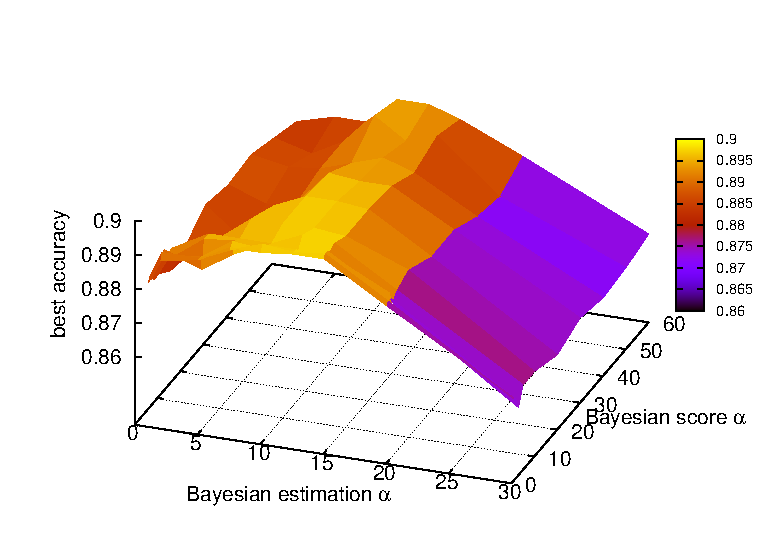
\includegraphics[scale=0.75]{fig/spam-holdout-whole-space-3d}
    \end{subfigure}
    \qquad
    \begin{subfigure}[b]{0.45\linewidth}
        \hspace{-1cm}
        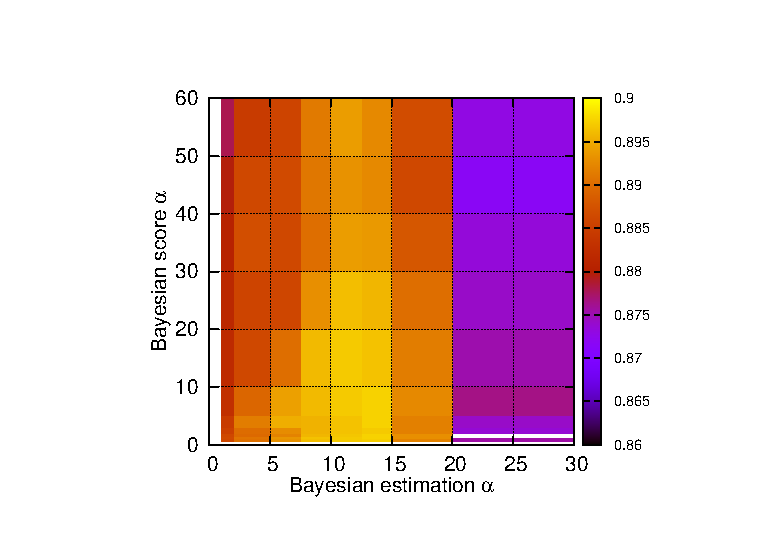
\includegraphics[scale=0.75]{fig/spam-holdout-whole-space-map}
    \end{subfigure}
    \caption{Accuracy of a Bayesian network model trained with different values of equivalent sample size $\alpha_S$ for structure learning (with Bayesian score) and for different values of $\alpha_P$ for parameter estimation (with Bayesian estimation).}
    \label{fig:spam-holdout-whole-space}
\end{figure}

\begin{comment}
\begin{figure}[ht]
    \centering
    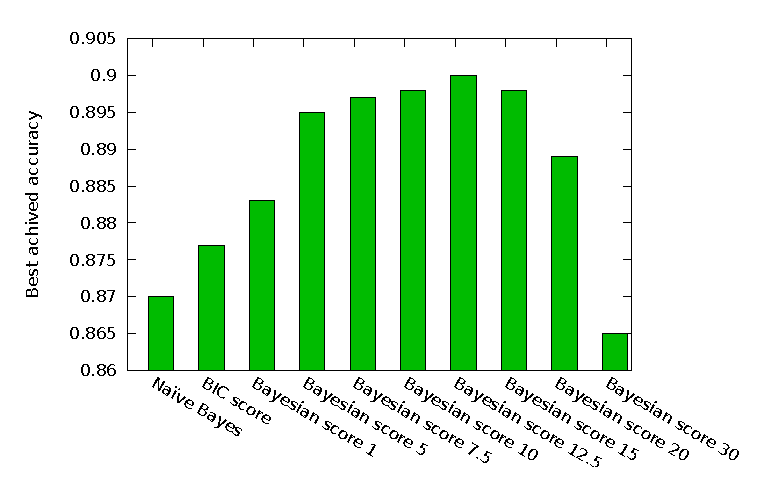
\includegraphics[scale=1]{fig/spam-holdout-best}
    \caption{Best accuracy achieved with Naïve Bayes model and with more general Bayesian networks learnt using different structure scores\,--\,BIC score and Bayesian score with different equivalent sample sizes. CPDs of each model have been computed using Bayesian estimation with equivalent sample size from the set $\lbrace 0.5, 1, 1.5, 2, 3, 5, 7.5, 10, 20, 30, 40, 50, 60 \rbrace$ and the best accuracy was chosen.}
    \label{fig:spam-holdout-testing}
\end{figure}
\end{comment}

Results of the 5-fold cross-validation are the following. Naïve Bayes model (parameters estimated via MLE) has the average accuracy 85.3\,\% which is by 3.7\,\% less than was reported for the Spambase dataset and Naïve Bayes in~\cite{renuka11} (reported 89\,\%). I believe this drop in accuracy is caused by discretization of the dataset and, in fact, it is almost surprising that the loss of variance isn't greater. Performance of the more general Bayesian network model has been inspected for parameter settings $(\alpha_S, \alpha_P) \in \lbrace 7.5, 10, 12.5, 15\rbrace \times \lbrace 7.5, 10, 12.5, 15 \rbrace$.
The best average accuracy from five-fold cross-validation has been 87.7\,\% with parameters $(\alpha_S, \alpha_P) \in \lbrace (15, 12.5), (15, 15) \rbrace$ which is by 2.4\,\% better than the accuracy of Naïve Bayes model. This result is comparable with the one achieved in~\cite{renuka11} through augmenting the Naïve Bayes model with a SVD-like preprocessing (reported increase of accuracy by 4\,\%).

Considering that the Spambase dataset is relatively small in size and provides only 57 features, it is very likely that better performance can be achieved with a bigger dataset and with a richer and carefully chosen set of features (the learnt Bayesian networks contained isolated variables suggesting that some of the features aren't correlated with the spam variable nor with any other and therefore are effectively useless).

Another authors have also shown that performance of probabilistic classifiers can be greatly improved by introducing a broader set of features including, for example, sender's domain, reverse DNS lookups, presence of HTML code in the body (also considering coloring, fonts), punctuation, currency characters, run-length of capital letters etc.~\cite{heckerman98_spam}

\medskip
Parameters of the structure learning procedure: 200 runs, 3\,000 iterations per run, 60 random restart steps, 0.15 relative size of tabu-list, maximum of three parents per variable, no incoming edges into the spam variable.


\subsection{Conclusion}
In this section I have demonstrated that a~Bayesian network can perform better than a~Naïve Bayes model in the field of spam detection even with a relatively small training set. Because both these models are very close in their nature and because Naïve Bayes model is so powerful that many real-world spam filters use it, I believe that with a large scale dataset a Bayesian network can achieve very high success rates. This is because the scoring functions for structure learning of Bayesian networks inherently make a good bias-variance trade-off depending on the size of our dataset and because we can further relax structural restrictions to increase possible variance of the Bayesian network model (in my experiments I disallowed the $spam$ variable to be a child and allowed up to three parents per node). Both these properties of Bayesian networks suggest that their true power in the field of spam detection lies with large datasets having rich sets of features, whereas the Naïve Bayes model has been repeatedly proved to perform excellently with small datasets which are common in practice.

\todo{There also exists an extension of Naïve Bayes, called Tree Augmented Naïve Bayes (TAM), that has the structure of Naïve Bayes model and furthermore allows for edges among attribute variables, as long as they don't form a V-structure. Advantage of TAM is that the optimal tree structure can be learnt in polynomial time whereas the learning of a more general Bayesian network, which I did, is generally NP-hard and therefore an optimization technique needs to be employed. (add citation, try to find a paper that employs TAM on spam)}


\ignore{
\bigskip

Best performance of Naive Bayes:
\begin{itemize}
    \item MLE(accuracy, precision, recall): (0.87, 0.82, 0.85)
    \item Bayesian estimation (\todo{refer to the largest network in part 1\,--\,ICU for clues on how to choose $\alpha$ for 3681 samples and 57 attributes + 1 label}, or find a network with cca 60 nodes (HEPAR~II) and perform the analysis and place here a graph of learning curves) ($\alpha$, accuracy, precision, recall): (0.1, 0.87, 0.82, 0.85), (0.25, 0.87, 0.82, 0.85), (0.5, 0.87, 0.82, 0.84), (1, 0.86, 0.82, 0.84), (2, 0.86, 0.82, 0.83), (5, 0.87, 0.83, 0.83), (10, 0.87, 0.83, 0.83), (20, 0.86, 0.83, 0.82), (30, 0.87, 0.84, 0.82), (40, 0.87, 0.84, 0.81)
\end{itemize}


Best performance of $spam$ parent-only, max 3 parents per node, BIC score:
\begin{itemize}
    \item MLE(accuracy, precision, recall): (0.873, 0.862, 0.807)
    \item Bayesian estimation($\alpha$, accuracy, precision, recall): (1, 0.875, 0.863, 0.813), (2, 0.875, 0.860, 0.815), (5, 0.873, 0.862, 0.807), (10, 0.873, 0.864, 0.804), (20, 0.875, 0.869, 0.804), (30, 0.875, 0.869, 0.804), (40, 0.877, 0.874, 0.804), (50, 0.876, 0.878, 0.796), (60, 0.877, 0.879, 0.799)
\end{itemize}

Best performance of $spam$ parent-only, max 3 parents per node, Bayesian score $\alpha=1$:
\begin{itemize}
    \item MLE(accuracy, precision, recall): (0.879, 0.875, 0.810)
    \item Bayesian estimation($\alpha$, accuracy, precision, recall): (0.5, 0.882, 0.876, 0.815), (1, 0.883, 0.876, 0.818), (1.5, 0.882, 0.876, 0.815), \todo{(2, 0.882, 0.876, 0.815)}, (3, 0.881, 0.875, 0.813), (5, 0.881, 0.875, 0.813), (10, 0.878, 0.872, 0.810), (20, 0.876, 0.872, 0.804), (30, 0.872, 0.870, 0.793), (40, 0.873, 0.875, 0.791), (50, 0.871, 0.872, 0.788), (60, 0.872, 0.875, 0.788)
\end{itemize}

Best performance of $spam$ parent-only, max 3 parents per node, Bayesian score $\alpha=2$:
\begin{itemize}
    \item MLE(accuracy, precision, recall): (0.871, 0.872, 0.788)
    \item Bayesian estimation($\alpha$, accuracy, precision, recall): (0.5, 0.889, 0.870, 0.846), \todo{(1, 0.891, 0.873, 0.848)}, (1.5, 0.890, 0.874, 0.843), (2, 0.891, 0.873, 0.848), (3, 0.887, 0.869, 0.840), (5, 0.889, 0.872, 0.843), (10, 0.884, 0.846, 0.837), (20, 0.890, 0.876, 0.840), (30, 0.888, 0.876, 0.835), (40, 0.889, 0.874, 0.840), (50, 0.886, 0.873, 0.832), (60, 0.883, 0.867, 0.829)
\end{itemize}

Best performance of $spam$ parent-only, max 3 parents per node, Bayesian score $\alpha=5$:
\begin{itemize}
    \item MLE(accuracy, precision, recall): (0.870, 0.869, 0.788)
    \item Bayesian estimation($\alpha$, accuracy, precision, recall): (0.5, 0.891, 0.879, 0.840), (1, 0.891, 0.877, 0.843), (1.5, 0.891, 0.877, 0.843), (2, 0.887, 0.875, 0.832), (3, 0.895, 0.882, 0.846), (5, 0.895, 0.882, 0.846), (7.5, 0.889, 0.876, 0.837), (10, 0.890, 0.879, 0.837), (20, 0.881, 0.871, 0.818), (30, 0.884, 0.874, 0.824), (40, 0.887, 0.878, 0.829), (50, 0.883, 0.870, 0.826), (60, 0.886, 0.873, 0.832)
\end{itemize}

Best performance of $spam$ parent-only, max 3 parents per node, Bayesian score $\alpha=7.5$:
\begin{itemize}
    \item MLE(accuracy, precision, recall): (0.875, 0.885, 0.785)
    \item Bayesian estimation($\alpha$, accuracy, precision, recall): (0.5, 0.896, 0.889, 0.840), (1, 0.895, 0.889, 0.837), (1.5, 0.897, 0.890, 0.843), (2, 0.893, 0.891, 0.829), (3, 0.896, 0.889, 0.840), (5, 0.895, 0.891, 0.835), (10, 0.897, 0.892, 0.840), (20, 0.893, 0.886, 0.835), (30, 0.886, 0.882, 0.821), (40, 0.888, 0.880, 0.829), (50, 0.888, 0.880, 0.829), (60, 0.886, 0.879, 0.824)
\end{itemize}

Best performance of $spam$ parent-only, max 3 parents per node, Bayesian score $\alpha=10$:
\begin{itemize}
    \item MLE(accuracy, precision, recall): (0.875, 0.876, 0.796)
    \item Bayesian estimation($\alpha$, accuracy, precision, recall): (0.5, 0.896, 0.880, 0.851), (1, 0.898, 0.885, 0.851), (1.5, 0.896, 0.878, 0.854), (2, 0.897, 0.883, 0.851), (3, 0.896, 0.883, 0.848), (5, 0.895, 0.884, 0.843), (10, 0.897, 0.887, 0.846), (20, 0.897, 0.887, 0.846), (30, 0.896, 0.885, 0.846), (40, 0.891, 0.879, 0.840), (50, 0.897, 0.890, 0.843), (60, 0.894, 0.886, 0.837)
\end{itemize}

Best performance of $spam$ parent-only, max 3 parents per node, Bayesian score $\alpha=15$:
\begin{itemize}
    \item MLE(accuracy, precision, recall): (0.882, 0.885, 0.804)
    \item Bayesian estimation($\alpha$, accuracy, precision, recall): (0.5, 0.897, 0.887, 0.846), (1, 0.898, 0.890, 0.846), (1.5, 0.898, 0.890, 0.846), (2, 0.898, 0.890, 0.846), (3, 0.897, 0.890, 0.843), (5, 0.898, 0.890, 0.846), (10, 0.896, 0.889, 0.840), (20, 0.896, 0.889, 0.840), (30, 0.895, 0.889, 0.837), (40, 0.891, 0.886, 0.832), (50, 0.894, 0.886, 0.837), (60, 0.891, 0.883, 0.835)
\end{itemize}

Best performance of $spam$ parent-only, max 3 parents per node, Bayesian score $\alpha=20$:
\begin{itemize}
    \item MLE(accuracy, precision, recall): (0.878, 0.886, 0.793)
    \item Bayesian estimation($\alpha$, accuracy, precision, recall): (0.5, 0.886, 0.884, 0.818), (1, 0.887, 0.887, 0.818), (1.5, 0.889, 0.885, 0.826), (2, 0.887, 0.882, 0.824), (3, 0.885, 0.884, 0.815), (5, 0.887, 0.887, 0.818), (10, 0.889, 0.887, 0.824), (20, 0.885, 0.881, 0.818), (30, 0.885, 0.879, 0.821), (40, 0.881, 0.871, 0.818), (50, 0.879, 0.875, 0.810), (60, 0.883, 0.881, 0.813)
\end{itemize}

Best performance of $spam$ parent-only, max 3 parents per node, Bayesian score $\alpha=30$:
\begin{itemize}
    \item MLE(accuracy, precision, recall): (0.858, 0.856, 0.796)
    \item Bayesian estimation($\alpha$, accuracy, precision, recall): (0.5, 0.865, 0.855, 0.793), (1, 0.864, 0.854, 0.791), (2, 0.863, 0.854, 0.788), (3, 0.860, 0.848, 0.785), (5, 0.865, 0.861, 0.785), (10, 0.865, 0.855, 0.793), (20, 0.862, 0.851, 0.788), (30, 0.865, 0.861, 0.785), (40, 0.863, 0.858, 0.782), (50, 0.864, 0.856, 0.788), (60, 0.866, 0.864, 0.785), (70, 0.863, 0.856, 0.785)
\end{itemize}

Best performance of $spam$ parent-only, max 3 parents per node, Bayesian score $\alpha=x$:
\begin{itemize}
    \item MLE(accuracy, precision, recall): (0., 0., 0.)
    \item Bayesian estimation($\alpha$, accuracy, precision, recall): (0.5, 0., 0., 0.), (1, 0., 0., 0.), (1.5, 0., 0., 0.), (2, 0., 0., 0.), (3, 0., 0., 0.), (5, 0., 0., 0.), (10, 0., 0., 0.), (20, 0., 0., 0.), (30, 0., 0., 0.), (40, 0., 0., 0.), (50, 0., 0., 0.), (60, 0., 0., 0.)
\end{itemize}
}
















\chapter{Conclusion}
This master's thesis explained the fundamentals of Bayesian networks, described various inference methods and methods of model learning. To get better hold of the theoretical concepts and to gain some insight I supplied commented formal proofs or derivations of multiple statements, some of the proofs were constructed by myself. All techniques have been studied and presented in such a detail that is fully sufficient in order to implement them and to understand their limitations.

The practical part of this thesis is divided into three areas.
The first area is a study of effects of different parameter settings of presented model learning methods for datasets and networks of various sizes. This study provides the reader with some intuition and hints on how to proceed when learning a network whose structure and/or CPDs are unknown.
The second practical part explores the possibility of using Bayesian networks as a tool for data-mining. Concretely, three models for the Crimes and Communities dataset have been learnt and we were able to observe close interaction of certain clusters of variables as well as their overall impact on criminality.
The third practical part examines the possibilities of using a Bayesian network in the field of spam detection and shows that a Bayesian network can outperform the very successful Naïve Bayes model, even with a relatively modest training set.

I believe that the most promising continuation of this thesis would be to thoroughly inspect the possibility of using Bayesian networks as spam detectors. In order to achieve better results a bigger dataset would be needed and extending the Bayesian network from discrete to continuous would also bring additional improvement.

\ignore{
\bigskip

My original contributions:
\begin{itemize}
	\item I myself devised some proofs and nice formal theories: Joint probability distribution induces by a BN indeed is a probability distribution (sums to one). Derivation of the formula for weighted sampling. Nice theory for finding all possible alterations of a network (for state-space search in structure learning).
\end{itemize}

What I did in the practical part:
\begin{itemize}
    \item I have demonstrated the analysis which should be performed if our goal is to learn network parameters as accurately as possible. I also examined relation of the ability to learn the \uv{true} structure and dataset size.
    \item A more general Bayesian network can perform better than Naïve Bayes model in context of spam filtering. Supposedly, mostly with large datasets (Bayesian network has higher variance).
\end{itemize}
}
%=========================================================================
%begin-of-inserted-footer









% Pouzita literatura
  % ----------------------------------------------
\ifczech
  \bibliographystyle{czechiso}
\else 
  \bibliographystyle{plain}
%  \bibliographystyle{alpha}
\fi
  \begin{flushleft}
  \bibliography{literatura} % viz. literatura.bib
  \end{flushleft}
  \appendix
   
  %\chapter{Notation overview}\label{ch:appendix_notation}
This chapter presents listing of the mathematical notation used in this thesis:

\bigskip
\begin{tabular}{ll}
	$X$ & Capital letter denotes a random variable.\\
	&\\
	$x$ & Lowercase letter denotes a concrete instantiation of the variable $X$.\\
	&\\
	$\vars{X}$ & Capital bold letter denotes a set of random variables.\\
	&\\
	$\vars{x}$ & Lowercase bold letter denotes an instantiation of all variables in the set $\vars{X}$.\\
	&\\
	$val(\vars{X})$ & Set of all possible instantiations of variables $\vars{X}$.\\
	&\\
	$Parents(X)$ & Set of parent variables of variable $X$ in a Bayesian network.\\
	&\\
	$parents(X)$ & Instantiation of parent variables of variable $X$ in a Bayesian network.\\
	&\\
	$Children(X)$ & Set of child variables of variable $X$ in a Bayesian network.\\
	&\\
	$children(X)$ & Instantiation of child variables of variable $X$ in a Bayesian network.\\
	&\\
	$N_x$ & Number of samples of a dataset for which variable $X$ has the value $x$.\\
	&\\
	$N_{x,\vars{pa}}$ & Number of samples of a dataset for which $X$ has the value $x$ and variables\\
	                  & $Parents(X)$ have the value $\vars{pa}$.\\
	&\\
	$\sum_\vars{X} (\dots)$ & Summation over instantiations $\vars{x}$ of the variables $\vars{X}$.\\
	&\\
	$P(\vars{X})$ & Probability distribution over variables $\vars{X}$.\\
	&\\
	$P(\vars{x})$ & Probability of variables $\vars{X}$ having the concrete instantiation $\vars{x}$.\\
\end{tabular}










\chapter{CD Content}\label{ch:appendix_cd_content}
Content of the enclosed CD is organized into the following directories:
\begin{itemize}
    \item \srccode{1-benchmarks/}: Network \srccode{.net} files, datasets and measurements related to the first practical application.
    \item \srccode{2-crime/}: Vector images of the final three networks that resulted from the analysis of criminality. Also contains the original dataset, its discretized version, networks learnt during the feature elimination process and records of analysis of the crime impact factor.
    \item \srccode{3-spam/}: Datasets (the original dataset, its discretized version, train and test sets for holdout testing and for 5-fold cross-validation). Also contains measurement records and figures.
    \item \srccode{program/}: Program source codes compilable using the \emph{ant} build tool and also runnable compiled version in \srccode{program/bin-precompiled}.
    \item \srccode{text/}:  {\LaTeX} sources of this thesis, including all figures.
\end{itemize} 





\chapter{Crime analysis\,--\,final networks}\label{ch:appendix_crime_net}
This chapter contains the three networks that are result of the crime analysis performed in Section~\ref{ch:practical_crime}. Because of their size, each network is on its own A3 page. If you have trouble reading variable names in the printed version please see the electronic version of this thesis or the original figures on the encolsed CD within the directory \srccode{2-crime/final networks/}.


\begin{hugepage}
\pdfpagewidth=2\pdfpagewidth
\begin{figure}[h]
    \centering
    \vspace*{-2.5cm}
    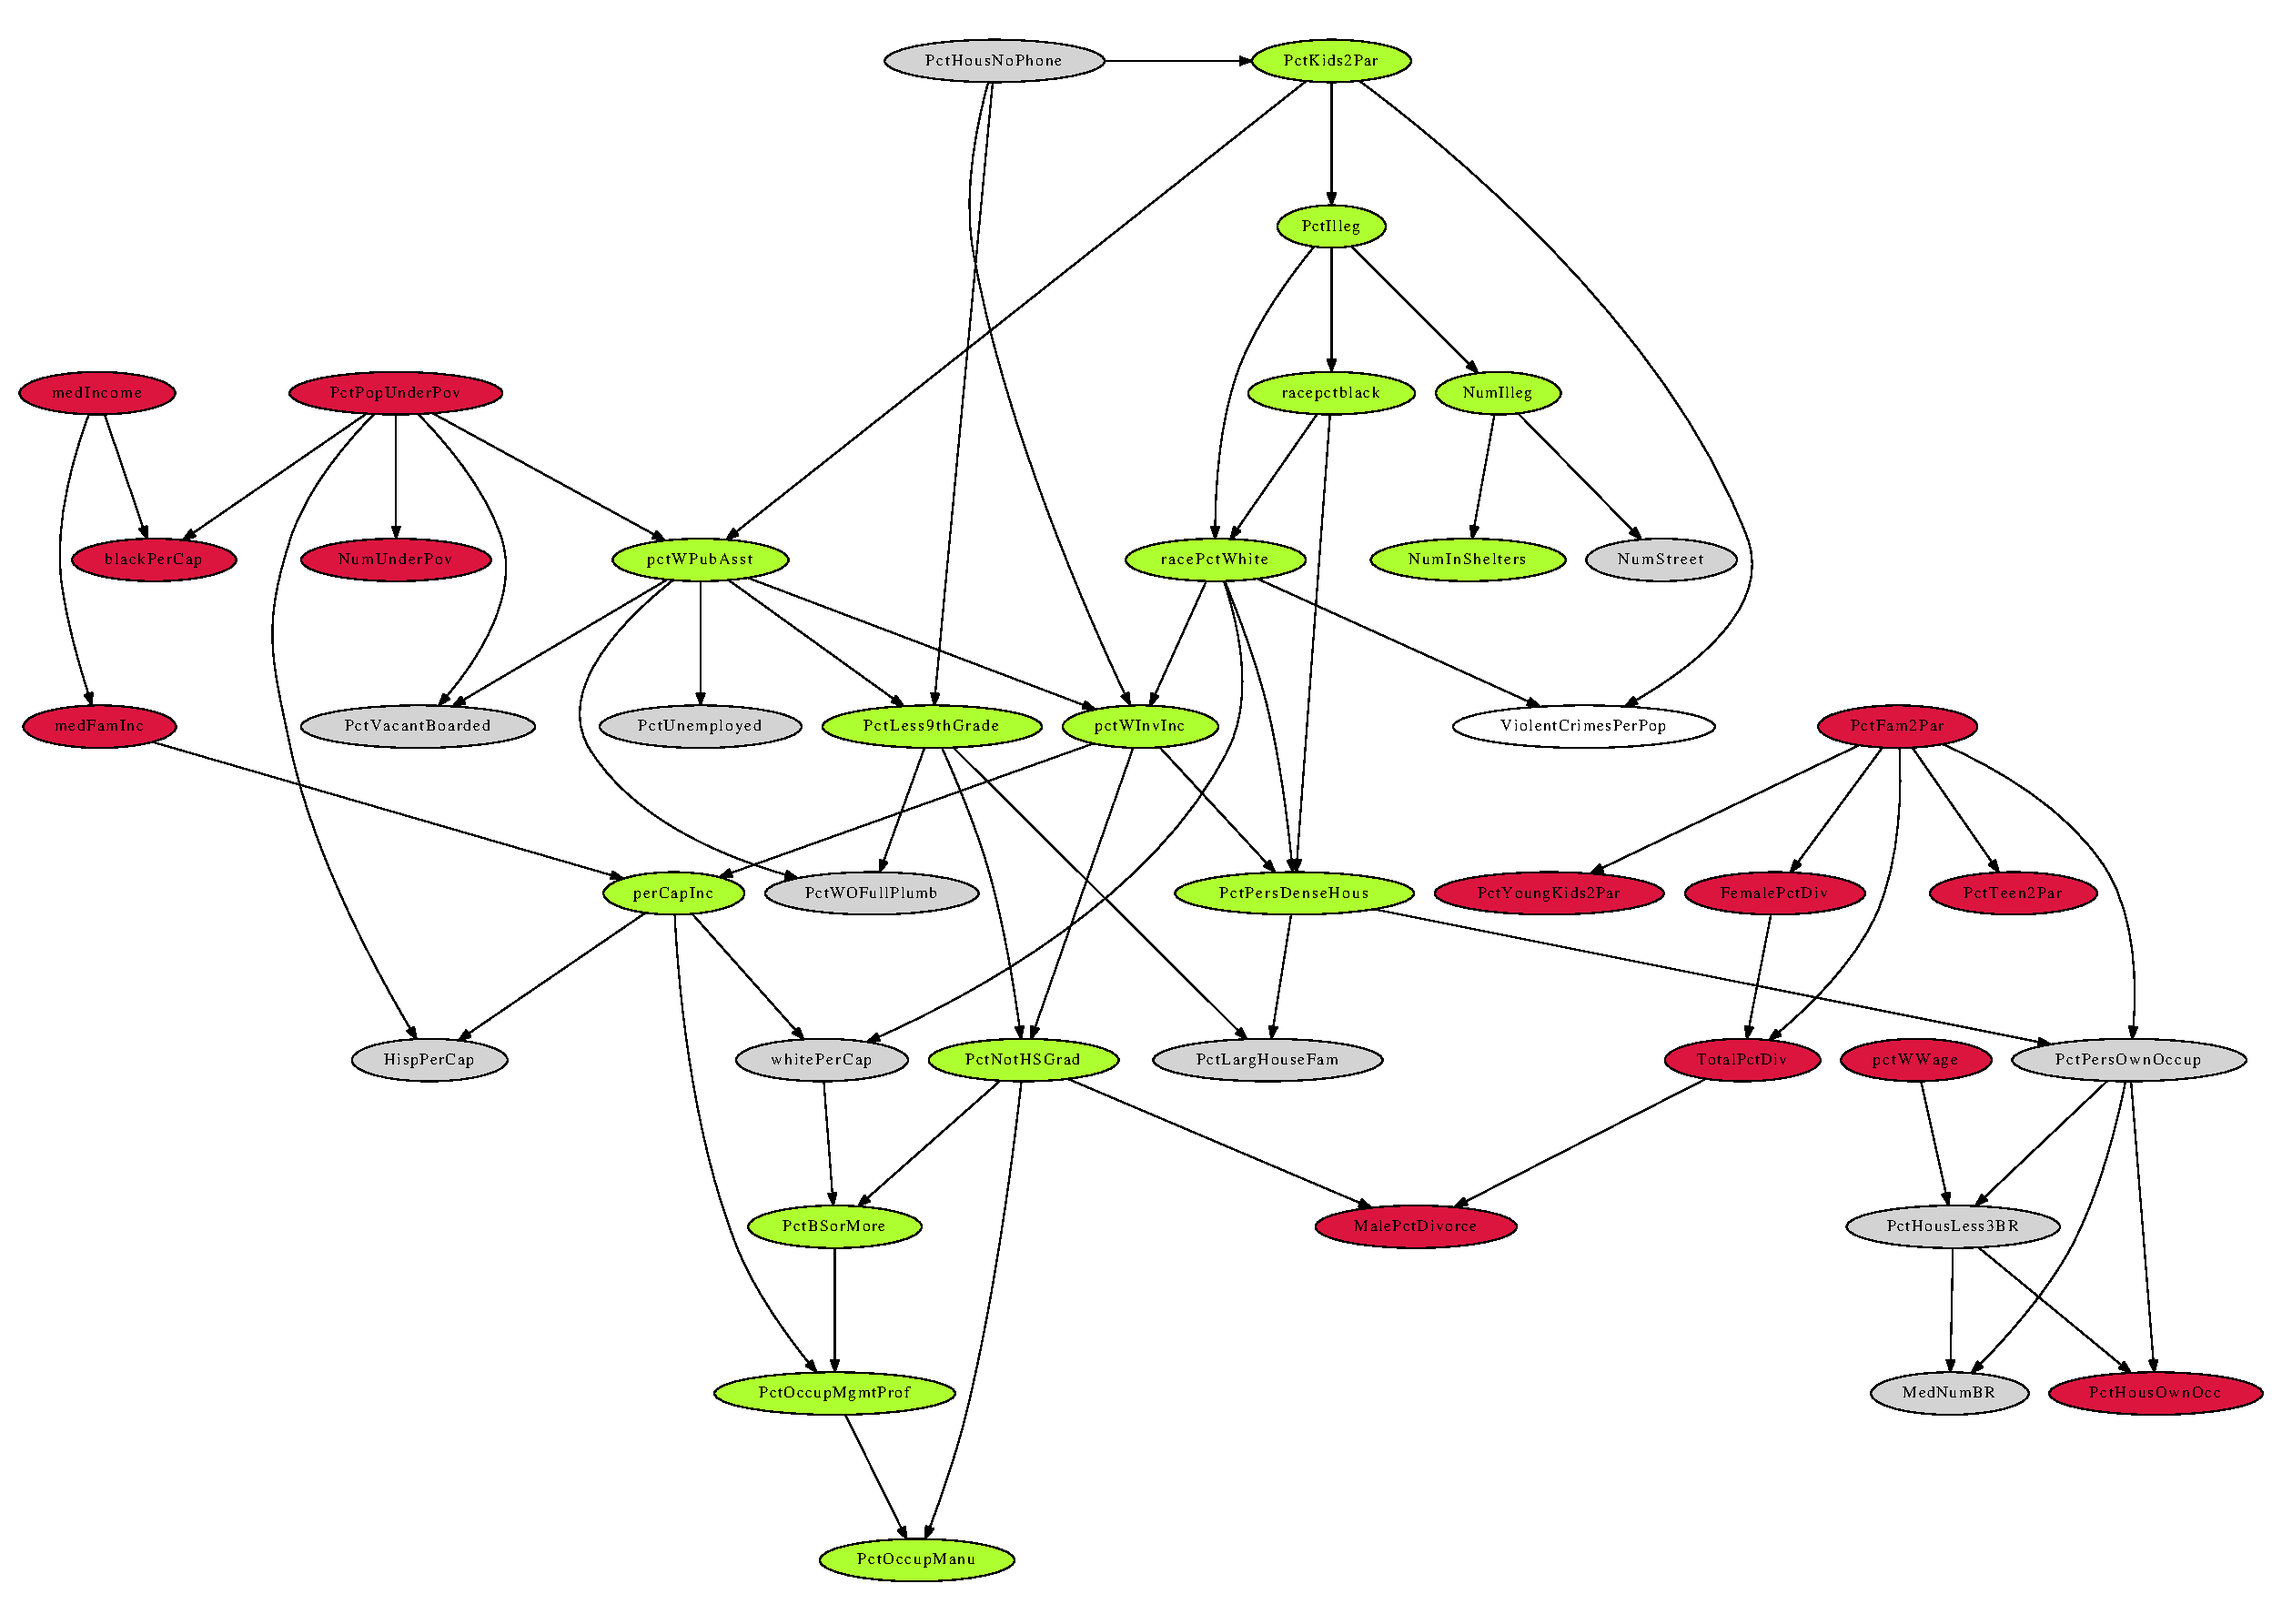
\includegraphics[scale=0.834]{fig/top-40_intersection_tolerance-1}
    \caption{Bayesian network for crime containing top 40 attributes with the highest crime impact factor.
    \\Legend: Green variables influence the $ViolentCrimesPerPop$ the same way as in the network with all 100 features. Influence of red variables is significantly different and therefore these variables shouldn't be considered.}
    \label{fig:crime_net_top40}
\end{figure}
\end{hugepage}

\begin{hugepage}
\pdfpagewidth=2\pdfpagewidth
\begin{figure}[h]
    \centering
    \vspace*{-2.5cm}
    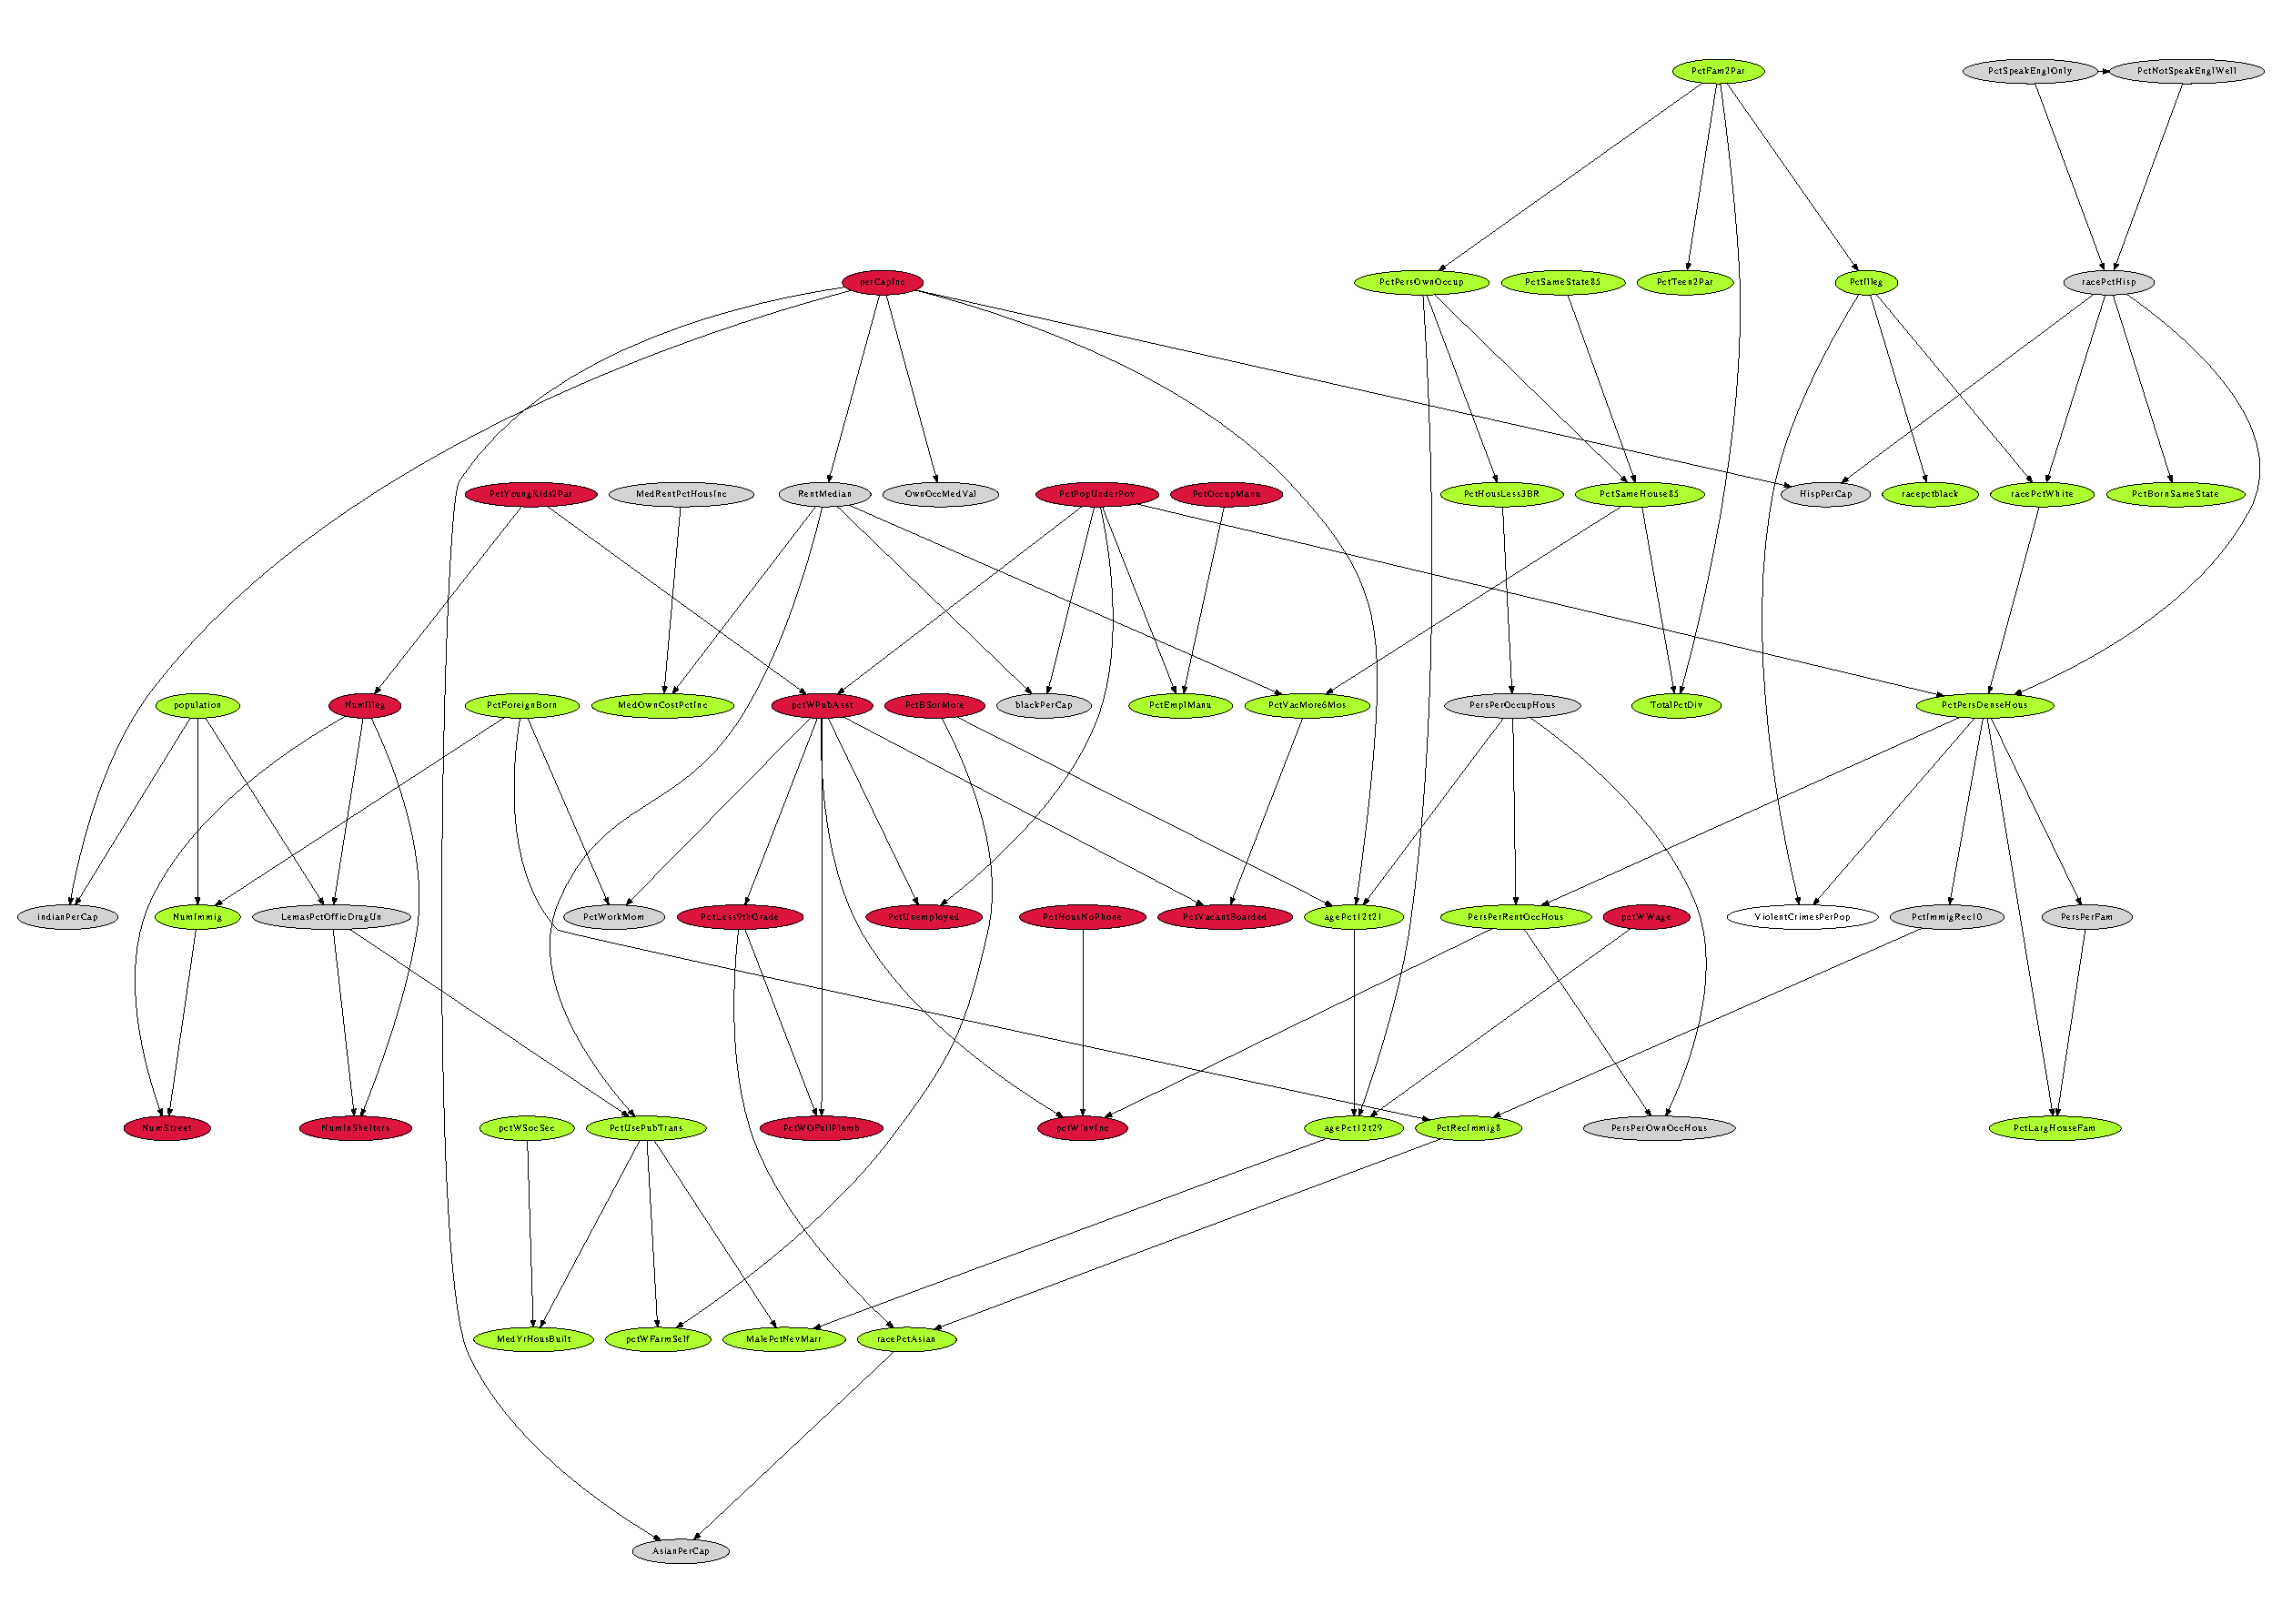
\includegraphics[scale=0.83]{fig/round-3_intersection_tolerance-1}
    \caption{Final Bayesian network for crime after three rounds of iterative elimination of similar variables.
    \\Legend: Green variables influence the $ViolentCrimesPerPop$ the same way as in the network with all 100 features. Influence of red variables is significantly different and therefore these variables shouldn't be considered.}
    \label{fig:crime_net_round3}
\end{figure}
\end{hugepage}

\begin{hugepage}
\pdfpagewidth=2\pdfpagewidth
\begin{figure}[h]
    \centering
    \vspace*{-2.5cm}
    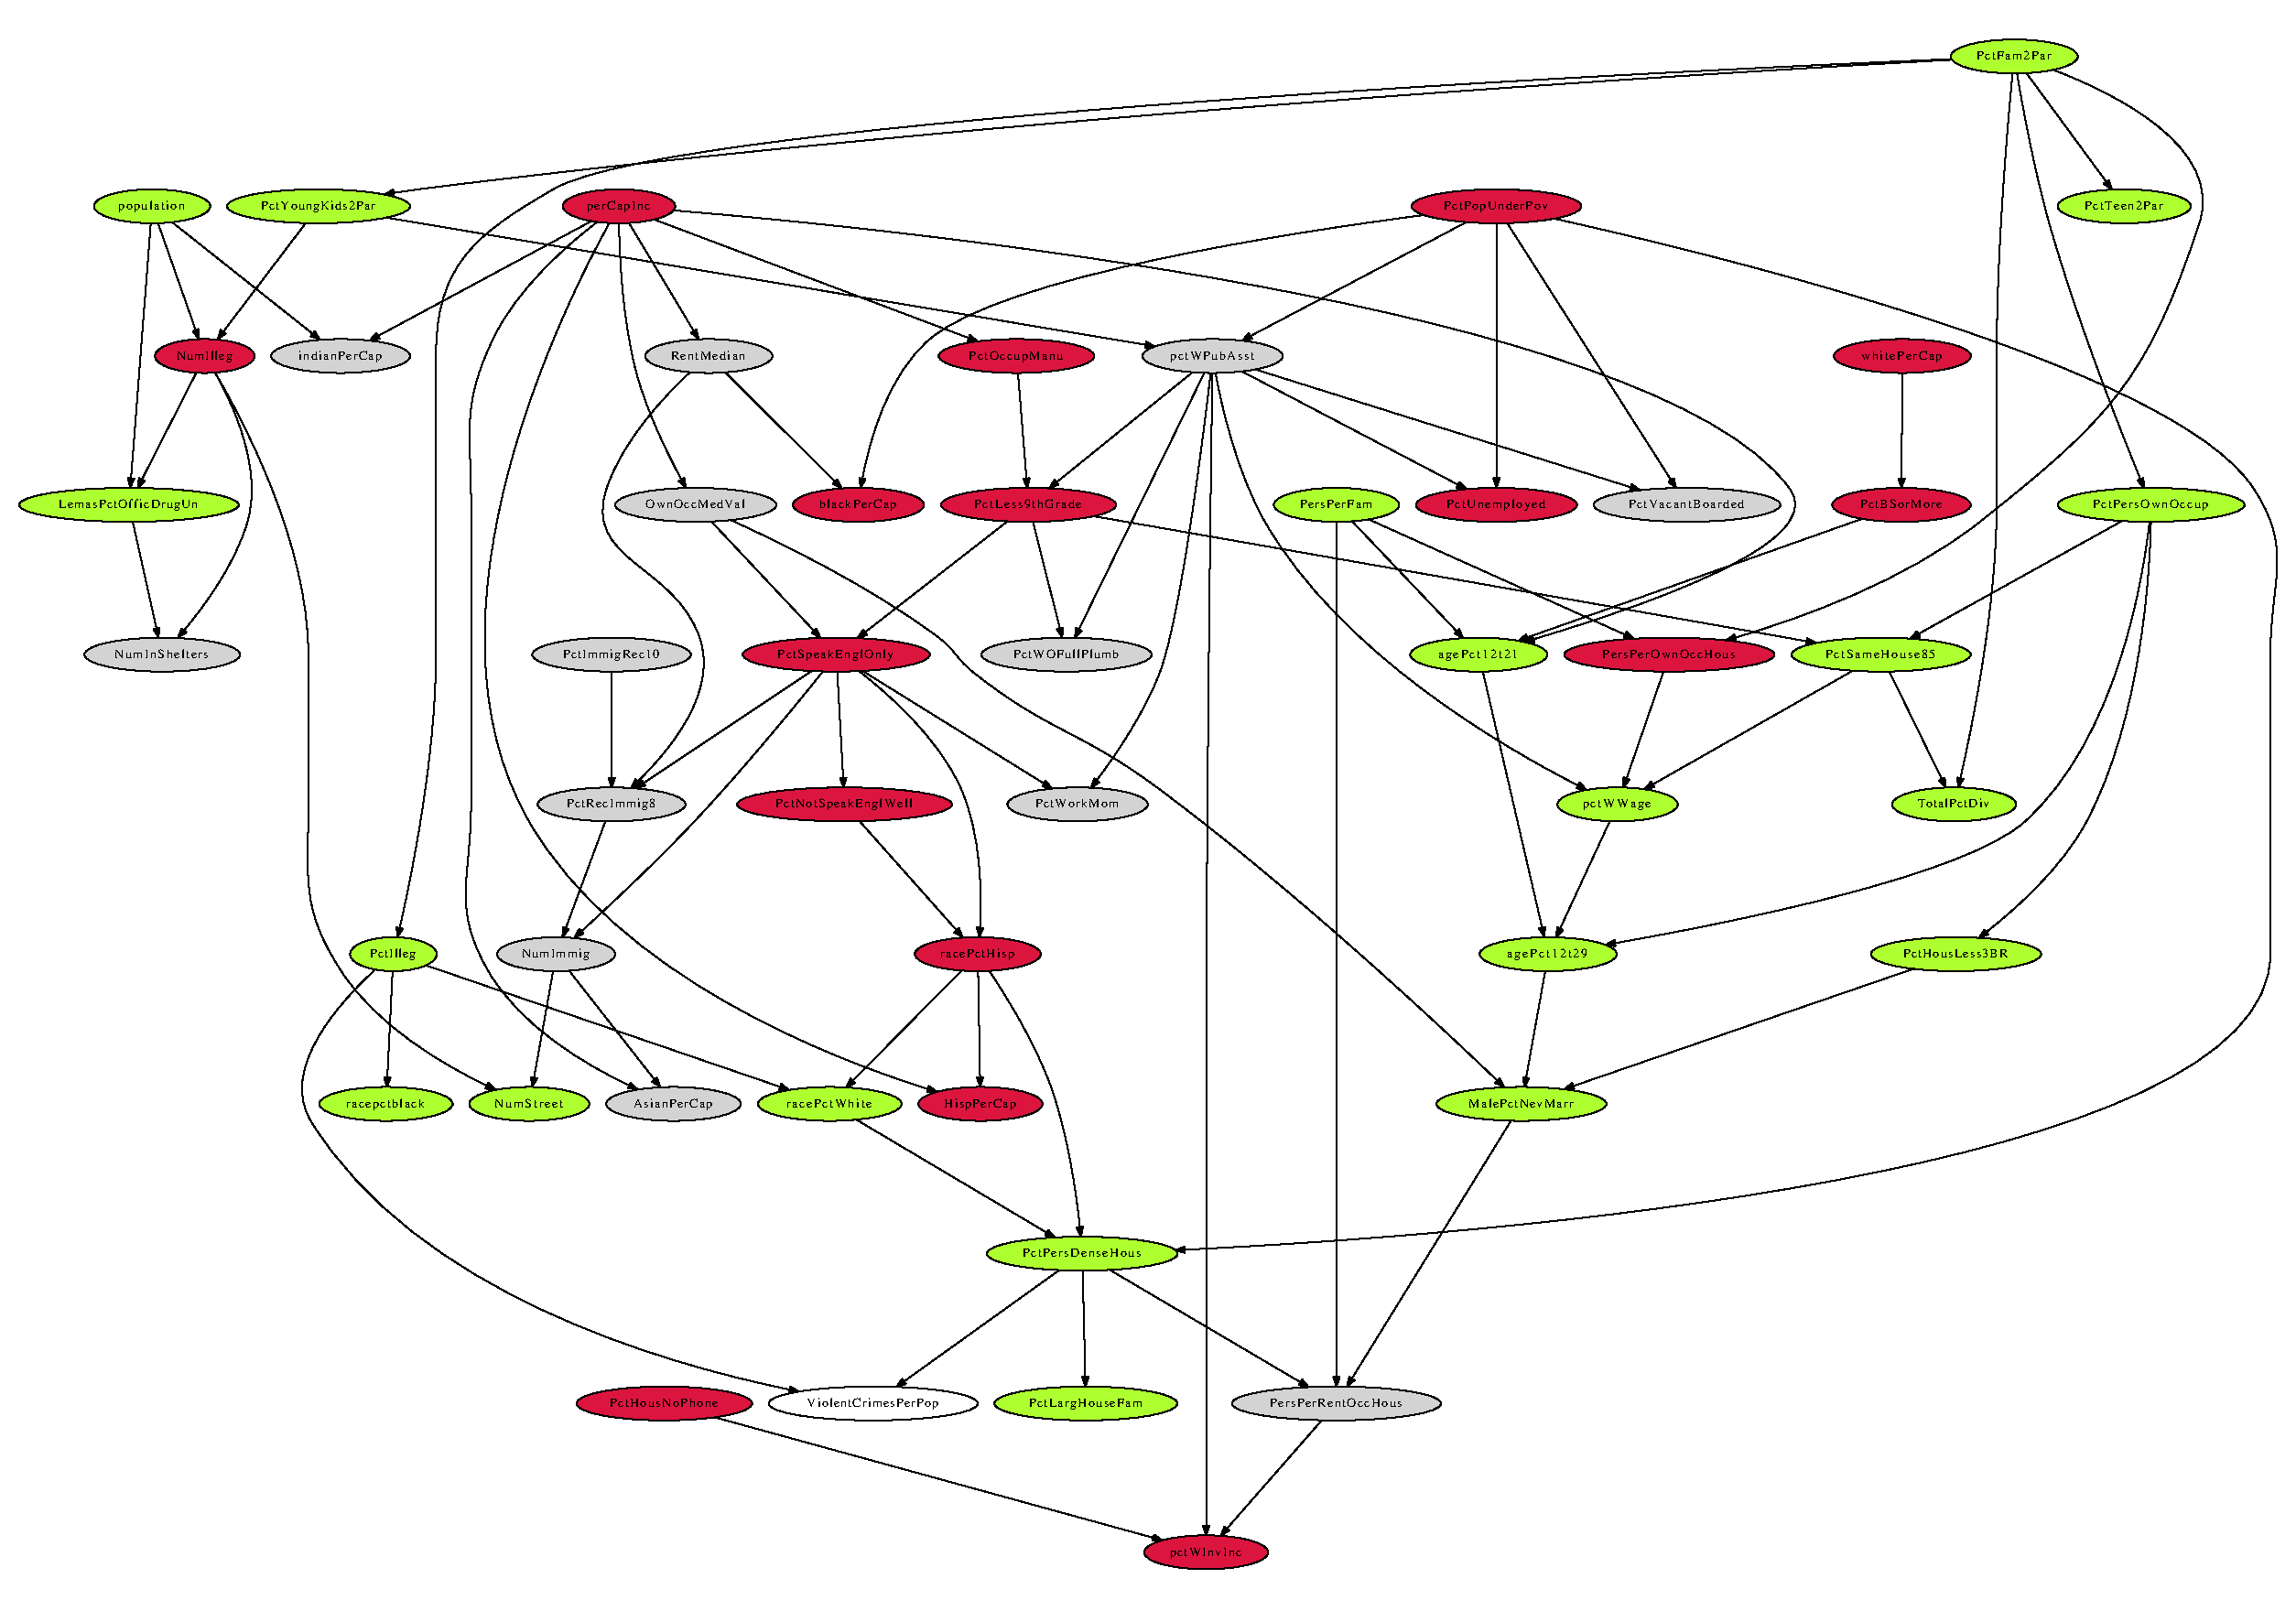
\includegraphics[scale=0.83]{fig/round-4_intersection_tolerance-1}
    \caption{Final Bayesian network for crime after three rounds of iterative elimination of similar variables and additional removal of variables whose crime impact factor is less than 0.07.
    \\Legend: Green variables influence the $ViolentCrimesPerPop$ the same way as in the network with all 100 features. Influence of red variables is significantly different and therefore these variables shouldn't be considered.}
    \label{fig:crime_net_round4}
\end{figure}
\end{hugepage}


 % viz. prilohy.tex
\end{document}
